\documentclass[10pt,xcolor=dvipsnames,mathserif]{beamer} 
\usepackage{rotating}
\usepackage[utf8]{inputenc}
\usepackage{amsmath}
\usepackage{slashed}
\usepackage{bm} % bold greek simbols
\usepackage{pifont}% http://ctan.org/pkg/pifont
\usepackage{booktabs}
\usepackage{comment}
\usepackage[force]{feynmp-auto}
\usepackage{multirow}
\usepackage{hyperref}
\usepackage{pgfpages}
%\setbeameroption{show notes on second screen} % Both
\setbeamertemplate{note page}{\pagecolor{yellow!5}\insertnote}\usepackage{palatino}
\usepackage{mathtools,calc}
\usepackage{appendixnumberbeamer}

\AtBeginSection[]
{
    \begin{frame}
        \frametitle{Table of Contents}
        \tableofcontents[currentsection]
    \end{frame}
}

% for fancy looking tables
\usepackage{booktabs} 

%Mine 
%\usetheme{Rochester}[height=200pt]
\usetheme{CambridgeUS}
\setbeamerfont{frametitle}{size=\small}
\useinnertheme[shadow=true]{rounded}
\useoutertheme[width=0pt]{sidebar}
\usecolortheme{whale}
\usecolortheme{orchid}
\setbeamercolor*{frametitle}{parent=palette primary}
%\setbeamerfont{frametitle}{size=\small}



%\setbeamertemplate{headline}[infolines theme] 
%\setbeamertemplate{footline}[page number]
%\setbeamertemplate{footline}[infolines theme] 
%\setbeamertemplate{items}[ball] 
%\setbeamertemplate{blocks}[rounded][shadow=true] 
\setbeamertemplate{navigation symbols}{} 


\setbeamercolor{structure}{fg=red!25!black} 
%\setbeamercolor{foot1}{fg=white, bg=red!65!black} 
%\setbeamercolor{foot2}{fg=white, bg=blue!25!black} 
%\setbeamercolor{foot3}{fg=white, bg=red!65!black} 

%\usetheme{Warsaw}
%\useinnertheme[shadow=true]{rounded}
%\useoutertheme[subsection=false]{miniframes}
%\usecolortheme{orchid}
%\usecolortheme{whale}

%\usetheme{Rochester}
%\DeclareOptionBeamer{height}{\PassOptionsToPackage{height=#1}{beamerouterthemesidebar}}
%\ProcessOptionsBeamer
%\useinnertheme{rectangles}
%\usecolortheme{whale}
%\usecolortheme{orchid}
%\setbeamerfont{block title}{size={}}
%\setbeamertemplate{headline}
%\useoutertheme[width=0pt]{sidebar}
%\useinnertheme{rectangles}

\graphicspath{{Images/}}

%
\newcommand{\U}[1]{\mathrm{U}(1)_{\mathrm{#1}}}			% Use this for U(1) groups
\newcommand{\SU}[2]{\mathrm{SU}(#1)_{\mathrm{#2}}}		% Use this for SU(N) groups
\newcommand{\SO}[2]{\mathrm{SO}(#1)_{\mathrm{#2}}}		% Use this for SO(N) groups
\newcommand{\E}[1]{\mathrm{E}_{#1}}		% Use this for Exeptional groupss
\newcommand{\g}[2]{g_{_\mathrm{#1}}^{#2}}
\newcommand{\mean}[1]{\left \langle #1 \right \rangle }
\newcommand{\abs}[1]{\left| #1 \right| }


% Stolen 
\usepackage{color}
\newcommand{\blue}[0]{\color{blue}}
\newcommand{\green}[0]{\color{ForestGreen}}
\newcommand{\red}[0]{\color{red}}
\newcommand{\magenta}[0]{\color{magenta}}
\newcommand{\brown}[0]{\color{brown}}
\newcommand{\cyan}[0]{\color{cyan}}
\newcommand{\purple}[0]{\color{purple}}
\newcommand{\cmark}{\ding{51}}%
\newcommand{\xmark}{\ding{55}}%



\titlegraphic{
	\vskip-5mm
	%
\includegraphics[height=1.5cm,keepaspectratio]{Logos/logoAveiro.jpg}
	%\hspace*{0.8cm}
	%\vspace{-.5cm}\hspace*{-1cm}
	%
\includegraphics[height=1.5cm,keepaspectratio]{Logos/2017_FCT_H_cor.jpg}
	%\hspace*{-0.3cm}
	%
\includegraphics[height=1.5cm,width=7.5cm,keepaspectratio]{Logos/logoProj.jpeg}\hspace*{0.05cm}
	%
\includegraphics[height=1.5cm,width=2cm,keepaspectratio]{Logos/cost.jpg}
	
\includegraphics[width=\textwidth,keepaspectratio]{Logos/g347.png}
}


\title[]{Phenomenological analysis in beyond the Standard Model theories: the cases of the minimal B-L-SM and of a BGL-like 3HDM}
\author[Pedro Rodrigues]{João Pedro Dias Rodrigues}
\institute{Universidade de Aveiro}
\date{26 of February of 2021}

% Remember the goal is to be done by day 26. 

\begin{document}
% ------ % 
\begin{frame}
  \titlepage
\end{frame}
% ------ % 
\note[itemize]{ {\Large
    \vskip5mm
    \item \textbf{Thank you} for being here to watch me present my thesis. 
    \vskip5mm
    \item My name is, Pedro. 
    \vskip5mm
    \item It is a phenomenological study of two Beyond the Standard Model frameworks.
    \vskip5mm
    \item One called the \textbf{B-L-SM} a simple unitary extension of the SM. 
    \vskip5mm
    \item and the other is a multi-Higgs Model called a \textbf{3HDM} with a flavour symmetry}
    }
% ------ % 
\begin{frame}
	\frametitle{General Structure}
	\tableofcontents
\end{frame}
% ------ % 
% Notes
\note[itemize]{ 
{\Large 
\item  We will begin by a short review of the role of SM in modern physics.  
\vskip8mm
\item I'll then quickly touch on flavour processes in the SM and show how they can be affected by new physics.
\vskip8mm 
\item Then we move to the B-L-SM where I'll present our results and conclusions.
\vskip8mm 
\item Finally we move onto the 3HDM where I will do the same. 
} }
\section{Modern Particle physics and the Standard Model} 
    % ------ % 
    \begin{frame}{Modern Particle physics}{The successes and failures of the Standard Model}
    %
    \begin{itemize}
        \item The conventional framework to describe all subatomic processes is the Standard Model  \textbf{(SM)}. \vskip3mm
        %%\pause 
        \vskip3mm
        \item  \textbf{However}, {\red \textbf{unanswered-questions}} have been revealed by modern experiments (LHC, Belle, Atlas, etc.). 
    \end{itemize}
    \vskip5mm
    %%\pause
    Some of these are:
    \begin{itemize}
        \item Deviations from it's theoretical predictions, e.g. \textbf{flavour deviations}, magnetic \textbf{moment anomalies in leptons} and others. 
        \item Others are conceptual in nature, \textbf{dark matter} and \textbf{neutrino masses} {\blue cannot} be explained by the SM. 
    \end{itemize} 
    %
    \vskip5mm
    %%\pause
    \begin{center}
        These problems lead scientists to look at the SM as a effective field theory and presents us with the possibility of \textbf{New Physics}!  
    \end{center}
    %
    \vskip2mm
    \begin{center}
    \textbf{The exploration of New Physics beyond the standard model is the quintessential work of theoretical physicists. } % A plethora of models are proposed to deal with the SMs issues.
    \end{center}
    \note[item]{ \Large The SM is the \textbf{fundamental tool} by which we can describe the interactions of particles. However recent experiments have revealed many problems with it. \vskip4mm }
    \note[item]{ \Large  Some are simply \textbf{deviations while other are conceptual flaws} that the SM cannot include within it's framework. \vskip4mm }
    \note[item]{ \Large  Given this physicists agree that there is a \textbf{call} for new physics \vskip4mm } 
    \note[item]{ \Large Which they explore in \textbf{Beyond the Standard Model} frameworks, like the ones we'll be studying here today.}
    \end{frame}
    % ------ %
    \section{Flavour processes in the Standard model} 
    \begin{frame}{The Standard Model - Flavour physics}{Flavour Changing Charged Currents}
        %
        \begin{center}
             The $W^\pm$ can {\blue mediate charge currents} to change the quark flavour! \\ These are called {\blue Flavour Changing Charged Currents (\textbf{FCCCs})}
        \end{center}
        %
        \begin{figure}[H]
            \centering
            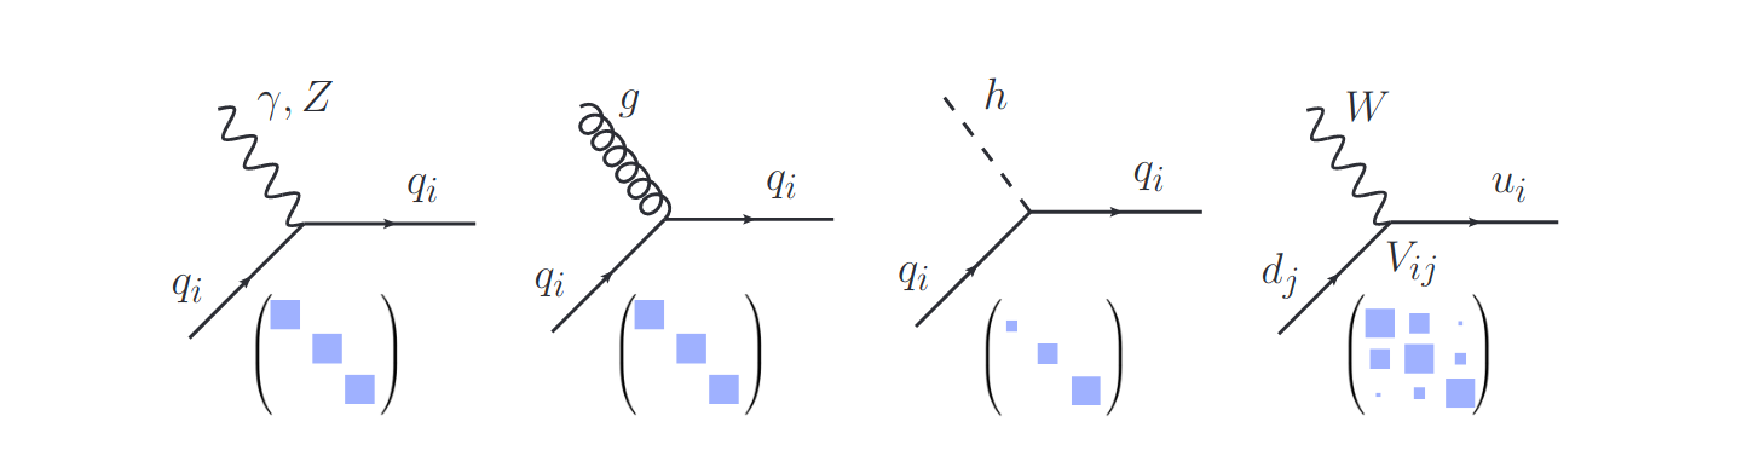
\includegraphics[width=1\textwidth]{TestYukawaCouplings(1).pdf}
        \end{figure}
        $W^\pm$ interactions with massive left-handed quarks fields follow from the terms, %%\pause 
        %
        \begin{equation*}
            \mathcal{L}_{kin}  \supset \frac{1}{\sqrt{2}} g \overline{u}^\prime_L \gamma^\mu V_{CKM} d_L^\prime W^+_\mu + \text{H.c.} \ , 
        \end{equation*}
        %
        Controlled by the CKM matrix which is defined as, $V_{CKM} = U^u_L U^{d ^\dagger }_L $. 
        \note[item]{ \large To quickly touch on flavour has we know \textbf{in the standard model the interactions trough zed boson, the photon, gluon and Higg are flavour diagonal and these participate in neutral currents.} However the $W^\pm$ can couple to the left handed quark fields and mix them due to them being SU2 doublets and represent \textbf{Flavour changing Charged Currents}. As we see here, these are only sources of quark flavour changing in the SM at tree-level  \vskip8mm }
        \note[item]{ \large And thanks to the redefinition of the physical quarks fields, the interactions between up and down quarks are controlled by the CKM matrix. \vskip8mm}
        %\note[item]{\Large   }
    \end{frame}
    %!%
    %\subsection{Flavour Physics}
    %!%
    % ------ %
    \begin{frame}{The Standard Model - Flavour physics}{Flavour Changing Neutral Currents}
        %
        However, in {\blue \textbf{higher order}} processes, it is possible to change flavour in neutral processes. These are called {\blue Flavour Changing Neutral Currents (\textbf{FCNCs})}. 
        %
        \begin{center}
            { \red These processes can be easily affected by new physics!} 
        \end{center}
        %
        \vskip1mm
        %
        \begin{figure}[h]
            \centering
        	\vspace{1em}
            \begin{minipage}{.49\textwidth}
                    \begin{fmffile}{decays_3}
                    \begin{fmfgraph*}(80,40)
                        \fmfset{arrow_len}{10}
                        \fmfstraight
                        \fmfleft{i3,i1}
                        \fmfright{o3,o2,o1}
                        \fmf{fermion}{i1,v1,o1}
                        \fmffreeze
                        \fmf{fermion,tension=1.5}{o3,v3,o2}
                        \fmf{phantom,tension=1.8}{i3,v3}
                        \fmflabel{b}{i1}
                        \fmflabel{c\,(s)}{o1}
                        \fmflabel{$\tau$ ($\mu^-$)}{o2}
                        \fmflabel{$\nu_\tau$ ($\mu^+$)}{o3}
                        \fmf{boson,label=H$^\pm ,, (Z^{\prime},,H^0_{new})$,label.side=left,foreground=(1,,0.1,,0.1)}{v3,v1}
                    \end{fmfgraph*}
                \end{fmffile}
            \end{minipage}
            %\hspace{1em}
            %
            \begin{minipage}{.3\textwidth}
                \begin{fmffile}{Decay_2222222222}
                    \begin{fmfgraph*}(100,60)
                    \fmfstraight
                    \fmfleft{b,i1,t}
                    \fmftop{tt1,tt2,tt3,tt4}
                    \fmfright{o1,o2,o3,o4,o5}
                    \fmf{fermion,tension=1,label=$b$}{i1,v1}
                    \fmf{fermion,label=$t$,label.side=left,tension=1}{v1,v3}
                    \fmf{fermion,tension=1}{v3,o5}
                    \fmf{dashes,tension=0.4,foreground=(1,,0.1,,0.1),label=$H^+$,label.side=right}{v1,v2}
                    \fmf{dashes,tension=0.4,foreground=(1,,0.1,,0.1),label=$H^0$,label.side=right}{v2,v3}
                    \fmf{dashes,tension=1.5,label=$H^-$,foreground=(1,,0.1,,0.1)}{v2,v4}
                    \fmf{fermion,tension=1.5}{o1,v4}
                    \fmf{fermion}{v4,o3}
                    \fmflabel{$\nu_\tau$}{o3}
                    \fmflabel{$\tau^-$}{o2}
                    \fmflabel{$c$}{o5}
                    \end{fmfgraph*}
                \end{fmffile}
            \end{minipage}
            \vspace{-1em}
        \end{figure}
        \vskip5mm
        \begin{center}
    		FCNCs can be very easily modified by new physics. Here we show, $b \rightarrow c \tau \nu$ and $b \rightarrow s \mu \mu$ transition. These processes show over $4\sigma$ deviations from their SM expected value. 
        \end{center}
        %
        \note[item]{ \large However what we will be more interested in is the higher order processes that we call flavour changing neutral currents. These are processes by which the quark flavour changes but the overall processes is neutral. These involve two w vertices in the SM.  \vskip2mm}
        \note[item]{These processes are particularly interesting because they are very rare suppressed by the GIM mechanism and loop order and are showing very high deviations.  \vskip2mm} 
        \note[item]{Which is particularly perfect because these processes can be easily modified by virtual new physics particles. \vskip2mm }
        \note[item]{\large Here we can see how exactly new physics can offer new processes at tree-level in the left case and at loop level in the right as to affect FCNCs. \vskip2mm }
        \note[item]{\large Note the procsses we see here are showing over 4 $\sigma$ deviations in the Standard Modle and are the the B into s $\mu \mu$ and the c into $\tau \nu$} 
    \end{frame}
        %


\section{The B-L-SM model.}
    %
    %!% 
    %\subsection{Motivation and Basic Framework}
    %!% 
    %
    % ------ %
    \begin{frame}{B-L-SM - Basics}{Introduction}
        %
        \begin{itemize}
            \item The SM contains an accidental symmetry that conserves {\blue \textbf{baryon minus lepton number}}. 
            \item In the {\blue B-L}-SM it is promoted to a symmetry and the SM gains a Abelian unitary group $\mathrm{U}(1)_{\mathrm{B-L}}$. 
        \end{itemize}
        %
        \begin{center}
            {\red Simple but deep!} $\longrightarrow$ {\green A great testing ground for computational tools} 
        \end{center}
        %
        %.%
        
        %.%
        %
        \vskip2mm
        %
        %%\pause 
        %
        \textbf{Motivations for ${\mathrm{B-L}}$ (Baryon number minus Lepton number) symmetry:}
        %
        \vskip2mm
        %
        \begin{itemize}
        	\item $\mathrm{B-L}$ symmetry relevant for baryogenesis through leptogenesis,
        	\item Grand Unified Theories, e.g.~$\SO{10}{}$, $\E{6}$, $\E{8},\ldots$ contain gauged $\U{B-L}$,
        	%\item The scale of $\U{B-L}$ breaking sets the mass scale of the right-handed Majorana neutrinos.
			%
			\item Enhanced vacuum stability compared to the SM.
        \end{itemize}
        %				
        \note[item]{ \Large The B-L-SM is a simple extension of the SM where a accidental symmetry gets promoted to a simple global unitary abelaian group, U 1 b-L we see here. \vskip6mm }
        \note[item]{ \Large However simple this model does offer a large set of phenomenological consequences. which are a great playground for our computational tools. \vskip6mm}
        \note[item]{\Large this addition is also very well motivated by GUT scenarios and cosmological implications. \vskip6mm}
    \end{frame}
    % ------ %
    \begin{frame}{B-L-SM - Basics}{BSM physics}
        %
        \begin{center}
            \textbf{New Physics} the B-L-SM offer: 
        \end{center}
        %
        \vskip2mm
        %
        \vskip3mm
        %
		\textbf{Three} generations of right-handed neutrinos $\to$ \textbf{\red no gauge anomalies}
		%
		\begin{itemize}
			\item Lightest is sterile and can be keV to TeV dark matter candidate. \\ % {\blue \scriptsize  Kaneta, Kang, Lee: JHEP 1702 (2017) 031}
			%\item Or stabilized via a $\mathbb{Z}_2^{\mathrm{DM}}$
			\item Type I See-saw mechanism as to address light neutrino masses.
		\end{itemize}
		%
        \vskip3mm
        %%\pause 
        Model contains a complex-singlet scalar $\chi$ whose VEV breaks $\U{B-L}$. 
        \begin{itemize}
            {\item \blue New \textbf{neutral scalar} $h_2$.}
        \end{itemize}
        %
        \begin{table}[h]
        \centering
        \begin{tabular}{|c|c|c|c|c|c|c|c|c|}
        \hline
        & $q_L$  & $u_R$ & $d_R$ & $l_L$  & $e_R$ & $\nu_R$  &  $H$  & $\chi$  \\ \hline
        $\mathrm{SU(3)_C}$& $\mathbf{3}$ & $\mathbf{3}$  & $\mathbf{3}$  & $\mathbf{1}$  & $\mathbf{1}$   & $\mathbf{1}$   & $\mathbf{1}$    & $\mathbf{1}$    \\
        $\mathrm{SU(2)_L}$& $\mathbf{2}$  & $\mathbf{1}$ & $\mathbf{1}$ & $\mathbf{2}$ & $\mathbf{1}$ & $\mathbf{1}$ & $\mathbf{2}$  & $\mathbf{1}$ \\
        $\mathrm{U(1)_Y}$ & ${1}/{6}$ & ${2}/{3}$  & -${1}/{3}$  & -${1}/{2}$ & -1 & 0 & ${1}/{2}$ & 0 \\
        $\mathrm{U(1)_{B-L}}$ & ${1}/{3}$ & ${1}/{3}$ & ${1}/{3}$  & -1  & -1 &-1  & 0 & 2  \\ \hline 
        \end{tabular}
        \end{table} 
        %%\pause 
        From $\U{B-L}$ an extra $Z^\prime$ gauge boson is added.
        \begin{itemize}
            \item ${\green \U{Y}} \times {\red \U{B-L}}$ gauge kinetic-mixing parameter
        \end{itemize}
        %
        %
        \note[item]{\large what exactly are the differences from the SM in this model. This is, what new physics does the B-L-SM has to offer?}
        \note[item]{\large  First, set of right handed neutrinos that can serve as dark matter and at the same time offer trough a see-saw mechanism a explanation of light neutrino masses.}
        \note[item]{\large  A  new complex singlet field that will be tasked with breaking the new unitary gauge symmetry added by the B-L-SM. Note that by it being SU2 singlet and not charged in hyper charge neither it or the EW vev will interfere with each other.}
        \note[item]{\large  The B-L-SM includes a very popular $Z^\prime$ boson given the new unitary gauge group. Which is allowed to mix with the remaining gauge bosons.}
    \end{frame}
    % ----- %
    \begin{frame}{B-L-SM}{General Goal of the Study}
        \begin{center}
            {\bf Study the mutual viability of the Scalar and Gauge sector}
            \vskip1em
            {\bf \red Not studied in the B-L SM for heavy $Z^\prime$}
        \end{center}
        %
        %.%
        
        %.%
        %
        \vskip1em
        %%\pause 
        \begin{center}
			{\bf \begin{center} BSM vector bosons and scalars contribute to $\bm{\left(g-2\right)_\mu}$ anomaly \end{center} }
        \end{center}
	    %\begin{exampleblock}{}

		%\end{exampleblock} 
		%%%%%%%%%%%%%%%%%%%%%%%%%
		\begin{figure}[!h]
			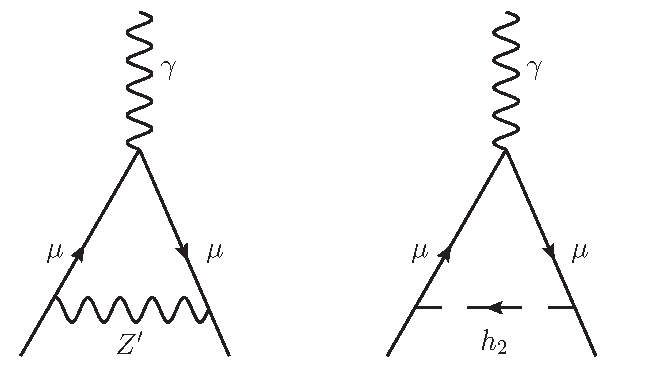
\includegraphics[scale=0.6]{g-2.pdf}
		\end{figure}	
		%%%%%%%%%%%%%%%%%%%%%%%%%			
		\begin{center}
		{\bf \red Not studied in the B-L SM} % (recently discussed in the supersymmetric version B-L SSM {\scriptsize \blue Yang, Feng et al. Phys.Rev. D99 (2019) no.1, 015002})
		\end{center}
		%
		%.%
		%
		%.% 
		% 
        %\begin{equation}
        %\Delta a_\mu = a_\mu^{\mathrm{exp}} - a_\mu^{\mathrm{SM}} = 268(63)(43) \times 10^{-11}
        %\end{equation}
        %\begin{center}
        %    Viability of a heavy $Z^\prime$
        %\end{center}
        \note[item]{\large So, what are our goal in studying such a simple model that is already rich in studies in the literature. Well first there was never a study of the scalar and gauge sector simultaneously for the case of a heavy $Z^\prime$. \vskip5mm } 
        \note[item]{\large Also never studied in the B-L-SM is the g-minus 2 anomaly for the B-L-SM in this case. This will be the primary focus of our studies given that }
    \end{frame}
    % ------ %


%\subsection{The working algorithm}

\begin{frame}{B-L-SM - Data analysis}{Range and procedure}
		%
		\begin{table}[htb!]
			\begin{center}
				\begin{tabular}{ccccc}
					\toprule                     
				 $\lambda_1$ & $\lambda_{2,3}$ & $g_{BL}$ & $g_{YB}$ & $x~\mathrm{[TeV]}$  
				 \\       
					\midrule
				$\left[10^{-2},\; 10^{0.5}
				\right]$	& $\left[10^{-8},\; 10
					\right]$ 			    							& $\left[10^{-8},\; 3
					\right]$		& $\left[10^{-8},\; 3
					\right]$	&	$\left[0.5,\; 20.5
					\right]$ 	\\
					\bottomrule
				\end{tabular}  
			\end{center}
		\end{table} 
		%
		\begin{enumerate}
			\item Model file: \texttt{SARAH-4.12.3}
			\item Spectrum generator: \texttt{SPheno-4.0.3}
			\begin{itemize}
				\item Unitarity
				\item One-loop mass spectrum and two-loop Higgs mass
				\item Mixing angles
				\item EW precision observables STU
				\item $\left(g-2\right)_\ell$ at one loop-level. 
				\item Decay widths and Branching Fractions
			\end{itemize}
			\item Generated points with $m_{h_1} \approx 125 ~\mathrm{GeV}$ input to \texttt{HiggsBounds-4.3.1} and  \texttt{HiggsSingnals-1.4.0}
			\item \textbf{Surviving} points passed to \texttt{MadGraph5$\_$amC5@NLO}
		\end{enumerate}
		%
		\note[item]{\large To perform these phenomenological studies we have developed a computational tool to scan the models parameter space. }
        \note[item]{\large Our code begins trough the use of SARAH, where we fed it all Lagrangian field and charge information so it can then generates a standard format model file to be fed to SPheno}
        \note[item]{\large SPheno is a fortran spectrum generator and with the information from Sarah generates a executable that quickly generates spectrum for a given set of parameters. Allowing us to study that specific parameter space point in great detail! Asides from the mass spectrum we need to highlight the unitarity constraints EW precision observables and decays-branching ratios etc.}
        \note[item]{\large We take this information to another set of programs called HiggsBounds and HiggsSignals and automatically assess the viability of the scalar sector.}
        \note[item]{\large All points that pass these constraints are fed into Madgraph where we test the most recent constraints for $Z^\prime$}
\end{frame}



%\subsection{Data-analysis for the B-L-SM}

%\end{comment}

\begin{frame}{B-L-SM - Data analysis}{$Z^\prime$ Constraints and its effect on the Higgs singlet}
    %%%%%%%%%%%%%%%%%%%%%%%%%%
\begin{figure}[!htb]
	\centering
	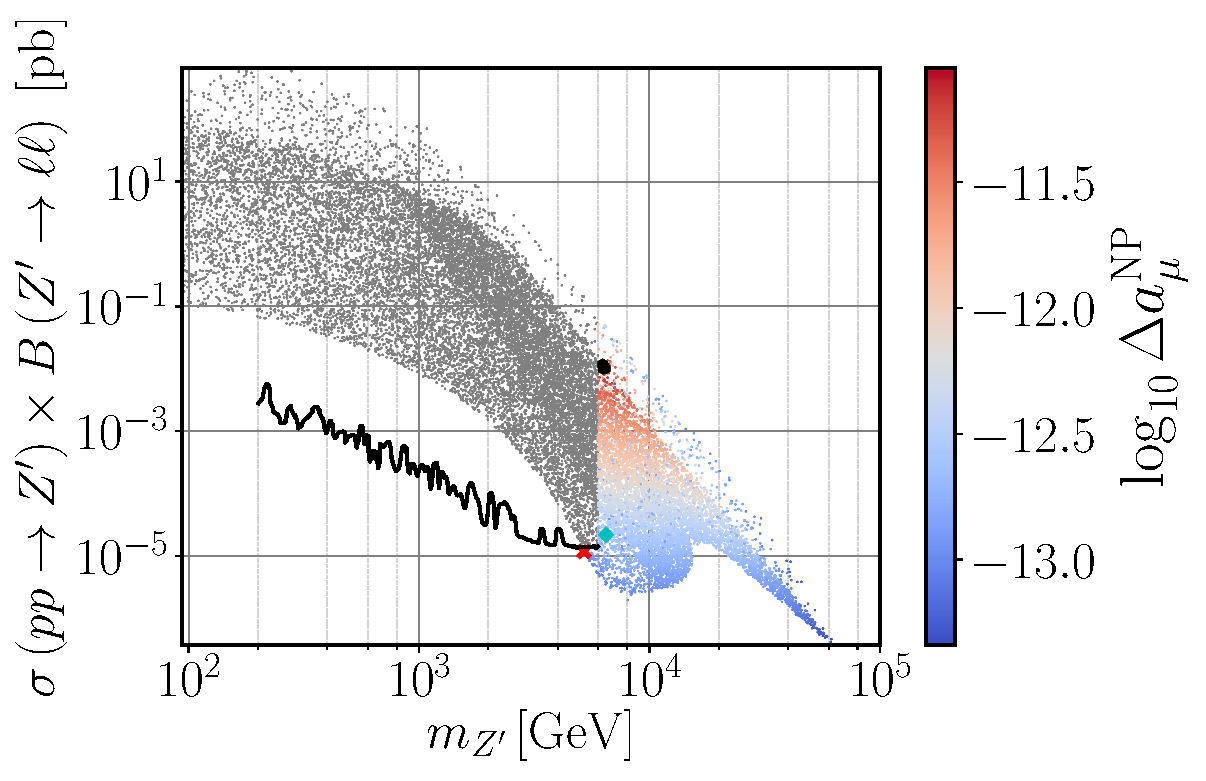
\includegraphics[width=0.45\textwidth]{Images/BLSM_2/mZp_Xsec_Amu.pdf}
	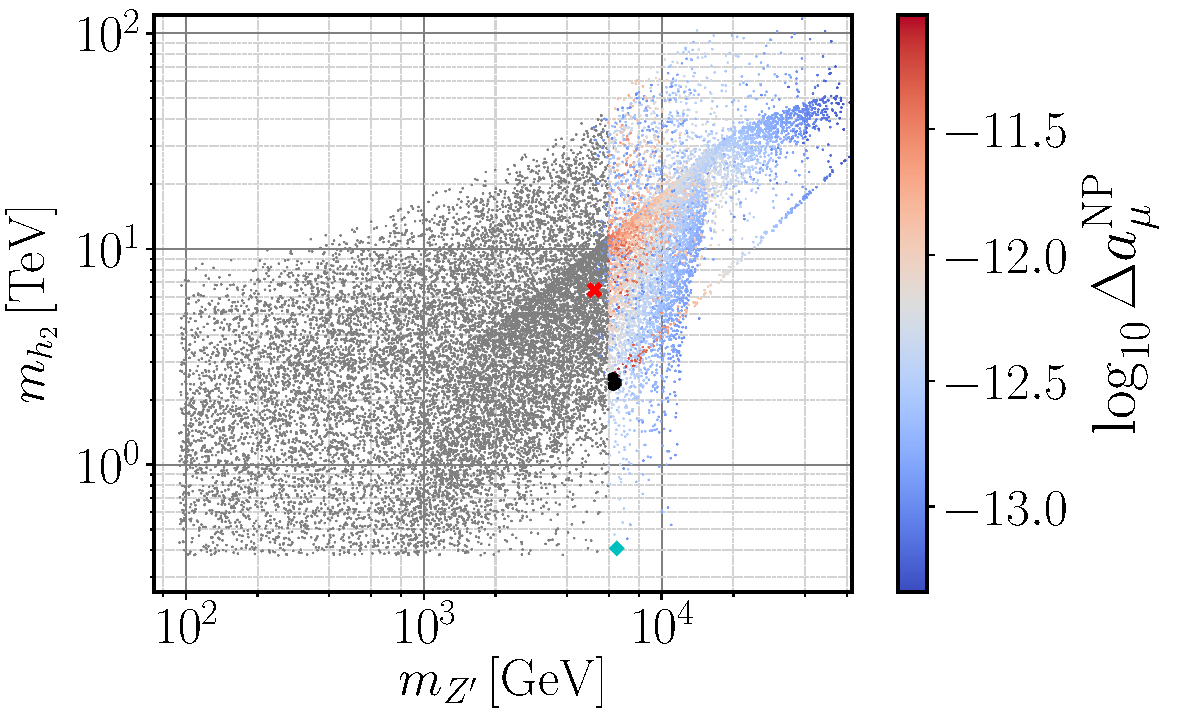
\includegraphics[width=0.45\textwidth]{Images/BLSM_2/mZp_Mhp_Amu.pdf}
	%\caption{Scatter plots showing the $Z^\prime$ Drell-Yan production cross section times the decay branching ratio into a pair of electrons and muons (left panel) and the new scalar mass $m_{h_2}$ (right panel) as functions of $m_{Z^\prime}$ and the new physics (NP) contributions to the muon $\Delta a_\mu$ anomaly. The solid line represents the current ATLAS expected limit on the production cross section times branching ratio into a pair of leptons at $95\%$ C.L.~ taken from Ref.~\cite{Aad:2019fac}.  Coloured points have survived all theoretical and experimental constraints while grey points are excluded by direct $Z^\prime$ searches at the LHC. These are represented by the red cross for the lightest $Z^\prime$ scenario (first row), cyan diamond for the lightest $h_2$ scenario (second row) and the black dots (last four rows).}
	\label{fig:Plots1}
\end{figure}	
%
%%%%%%%%%%%%%%%%%%%%%%%%%%

		\vskip-2mm
		\begin{itemize}
			\item Applied LEP constraints from 4 fermion contact interactions
			\vskip2mm
			\item {\bf Model shows a maximum $\Delta a_\mu^{\mathrm{NP}}$ of $8.9 \times 10^{-12}$ representing a marginal of the SM value for $\bm{6.3 ~\mathrm{TeV} \lesssim m_{Z^\prime} \lesssim 6.5~\mathrm{TeV}}$ (black dots).}
			\vskip2mm
			\item Red cross highlights a benchmark point with $m_{Z^\prime} \approx 5.2~\mathrm{TeV}$ and $m_{h_2} \approx 6.4~\mathrm{TeV}$ regarded as an early-discovery (or early-exclusion) scenario in future LHC runs.
			\vskip2mm
			\item Magenta diamond corresponds to the lightest BSM Higgs found, $m_{h_2} \approx 410~\mathrm{GeV}$
		\end{itemize}
	\note[item]{\large We took the points that passed STU unitarity and Higgs direct searches and found the corresponding plots after running them trough madgraph now we can check all surviving points against most recent $Z^\prime$ direct searches for lepton production and fermion contact interactions. Note that all grey points have a viable scalar sector. We begin to see the effect of combining direct searches from both sectors. Given the literature conditions we have effectively we have found the only remaining parameter space available for the B-L-SM.}
	\note[item]{\large Looking at these plots in finner detail we also see the principal conclusion of the B-L-SM. There is no way to fully explain the g-2 anomaly unlike we initially believed given modern limits. The best g-2 points are highlighted in black. They represent a improvement to about 3.3 sigma of the SM. }
	\note[item]{\large We also highlight that although there is no way of having a $Z^\prime$ lighter than 6.3 TeV there is a early discovery point with 400 GeV scalar. These are the blue cross and red square respectively. }
\end{frame}

\begin{frame}{so much so}
  %  $\Delta a_\mu^{Z^\prime}$ calculated in \texttt{SARAH} and numerically evaluated in \texttt{SPheno}
%			\vskip2mm				
\begin{itemize}
	\item When $\tfrac{m_\mu}{m_{Z^\prime}} \ll 1 $ the $Z'$ contribution reads
\end{itemize}
				\begin{equation*}
				\Delta a_\mu^{Z^\prime} \approx -\tfrac{1}{3 \pi^2} {\red \tfrac{m_\mu^2}{m_{Z^\prime}^2}} \left[6 \g{L}{\mu \mu Z^\prime} \g{R}{\mu \mu Z^\prime} - 4 \left({\g{L}{\mu \mu Z^\prime}}^2 + {\g{R}{\mu \mu Z^\prime}}^2\right) \right]\,
				\end{equation*}
				%Expanding for $v \ll x$
$$\g{L}{\ell \ell Z^\prime} \simeq \g{B-L}{} + \dfrac{1}{2} \g{YB}{}\,,
\qquad
\g{R}{\ell \ell Z^\prime} \simeq \g{B-L}{} + \g{YB}{}\,.$$
\vskip2mm
		
			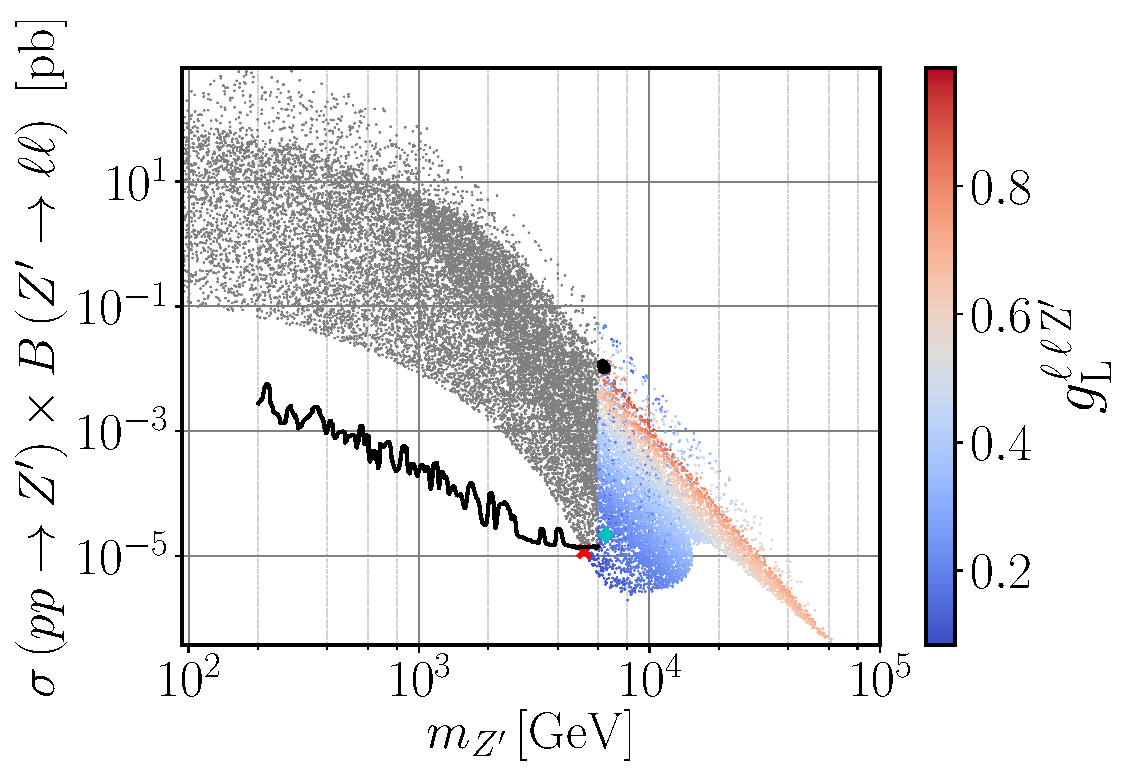
\includegraphics[width=0.32\textwidth]{Images/BLSM_2/mZp_Xsec_gLmumuZ.pdf}
	        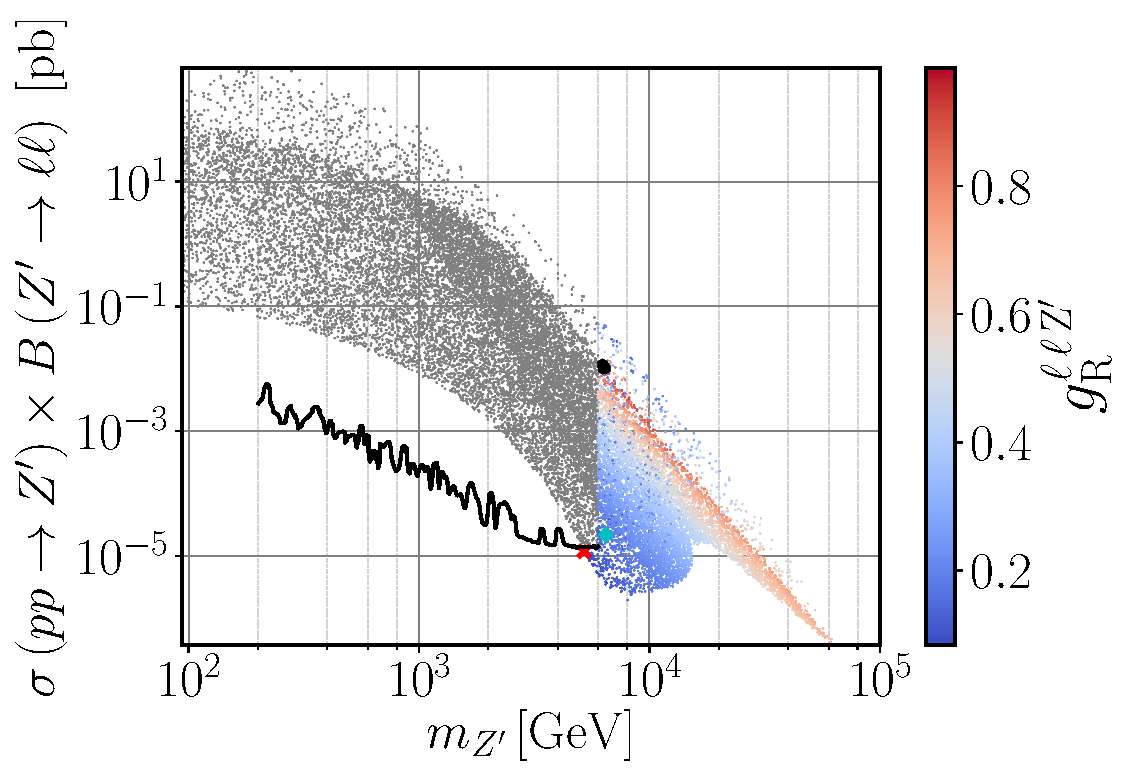
\includegraphics[width=0.32\textwidth]{Images/BLSM_2/mZp_Xsec_gRmumuZ.pdf}
	        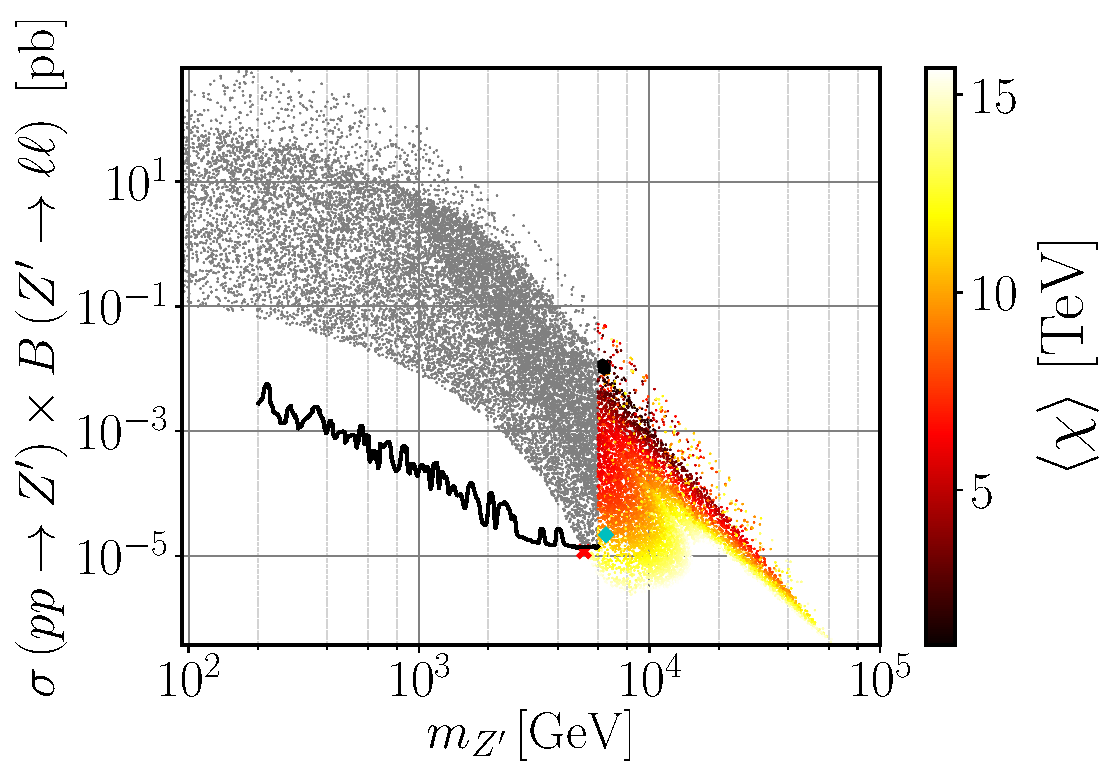
\includegraphics[width=0.32\textwidth]{Images/BLSM_2/mZp_Xsec_VEV.pdf}

\begin{itemize}
	\item Note strong correlation between $\red v/x$ and $\Delta a_\mu^{Z^\prime}$ except for the sparser upper edge!
	\item Strong correlation between the physical coupling to left and right handed fermions.
\end{itemize}
\note[item]{\Large However unlucky we must try to understand what conditions lead us to not have enough g-2 anomalous moment. First let us say that the h2 contributions are subleading and evaluate the Z prime contributions. Has expected these depend on the coupling to the muons of the z prime and the mass ratio of the Z prime with muons. Note the mass relation can be approximated to the VEV ratio which we see is directly inversely connected to the region with large a-mu with expected but also that there is a region with high left and right handed couplings to muons that is directly connected to the $a_\mu$ region.}
\note[item]{This is all has expected, our main conclusion here is that due to the EW constraints these couplings cannot be large enough to compensate the available VEV range. }
\end{frame}

\begin{frame}{B-L-SM - Data analysis}{Bench-marks}
    \setlength{\tabcolsep}{2pt} % Default value: 6pt
\renewcommand{\arraystretch}{1} % Default value: 1
%
\begin{table}[htb!]
\begin{center}
		\begin{tabular}{cccccccccc}
		\toprule
			$m_{Z^\prime}$ & $m_{h_2}$ &  $x$& $ \log_{10} \Delta a_\mu^{\mathrm{NP}}$ & $\sigma B$ & $\theta_W^\prime$ & $\log_{10}\alpha_h$ & $\g{B-L}{}$ & $\g{YB}{}$ & 
			$ \g{L}{\ell \ell Z^\prime} $% = \g{R}{\ell \ell Z^\prime}$ % & $\delta$ 
			\vspace{1mm}
			\\
			\hline \vspace{-1mm} \\ 
			%%%%%%%%%%
{ \red $5.199$ }   & $6.41$     & $15.4$    & $-13.01$       & $1.16 \mathrm{E}{-5}$   & $\approx 0$                    & $-5.18$     & $0.17$   & $2.0\mathrm{E}{-5}$    & $0.08$  %  &   $2.35\sigma$  
\vspace{1mm}  \\ 
 $6.478$    & { \cyan $0.41$ }    & $9.77$    & $-12.57$       & $2.15 \mathrm{E}{-5}$   & $3.22\mathrm{E}{-7}$      & $-5.85$     & $0.34$   & $1.7\mathrm{E}{-3}$    & $0.17$   %  &   $2.35\sigma$ 
\vspace{1mm}   \\ 
$6.371$    & $2.34$     & $1.08$   & $\mathbf{-11.05}$        & $0.01$                           & $1.05\mathrm{E}{-6}$      & $-7.31$     & $1.97$   & $2.1\mathrm{E}{-3}$    & $0.98$   %  &  $2.34\sigma$ 
\vspace{1mm}    \\ 
$6.260$    & $2.31$     & $1.15$   & $\mathbf{-11.07}$        & $0.01$                           & $5.87\mathrm{E}{-5}$      & $-2.79$     & $1.87$   & $0.125$                        & $0.94$  %  &  $2.34\sigma$  
\vspace{1mm}   \\ 
$6.477$    & $2.40$      & $1.14$   & $\mathbf{-11.08}$       & $0.01$                           & $2.75\mathrm{E}{-5}$      & $-4.29$     & $1.93$   & $0.06$                          & $0.97$  %  &  $2.34\sigma$ 
\vspace{1mm}    \\ 
$6.252$    & $2.53$     & $1.28$   & $\mathbf{-11.08}$        & $0.01$                           & $\approx 0$                    & $-8.65$     & $1.86$   & $1.6\mathrm{E}{-5}$     & $0.93$   %  &  $2.34\sigma$ 
\vspace{1mm}   \\ 
\bottomrule
\end{tabular}
		%\caption{A selection of five benchmark points represented in Figs.~\ref{fig:Plots1} and \ref{fig:Plots4} to \ref{fig:Plots2}. The $m_{Z^\prime}$, $m_{h_2}$ and $x$ parameters are given in TeV. The second line represents a point with lightest possible $h_2$ while the first one shows the lightest allowed $Z^\prime$ boson found in our scan. The last four lines show four points that yield a minimal tension $3.28$ standard deviations, with the combined theoretical and experimental error of the muon $(g-2)_\mu$ anomaly.}
		\label{tab:bench}
\end{center}
\end{table}
\setlength{\tabcolsep}{6pt} % Default value: 6pt
\renewcommand{\arraystretch}{1} % Default value: 1
	\vskip4mm
	\begin{itemize}
		\item \textbf{First line:} Early discovery/exclusion scenario with the lightest $Z'$ found in the scan,
		\vskip2mm
		\item \textbf{Second line:} Lightest new scalar found in the scan,
		\vskip2mm
		\item \textbf{Third to fourth lines:} Four best $\left(g-2\right)_\mu$ points. 
	\end{itemize}
	\note[item]{\Large A selection of five benchmark points represented here, the second line represents a point with lightest possible $h_2$ while the first one shows the lightest allowed $Z^\prime$ boson found in our scan.} 
	\note[item]{\Large The last four lines show four points with the best anomaly standing at around 3.3 sigma deviations from the SM value.}
\end{frame}

%\subsection{B-L-SM conclusions}

\begin{frame}{B-L-SM}{Conclusions and outlook of the B-L-SM}
	\textbf{\purple The $\left(g-2\right)_\mu$ anomaly:}
\begin{itemize}
	\item A heavy $Z'$ between $6$ and $8~\mathrm{TeV}$ cannot fully explain the anomaly
	%\item Needs sizeable kinetic-mixing parameter $\g{YB}{}$ which could reveal a $Z'$ boson.  
	\item There is still the need to consider electron anomalous magnetic moment.
	\item Small remaining parameter space, model likely completely excluded by the new LHC III upgrade. 
\end{itemize}
\vskip2mm
	\textbf{\purple New physics searches}
\begin{itemize}
	\item We have identified 6 benchmark points to test the B-L SM at future LHC searches:
	\vskip2mm
	\begin{itemize}
		\item For a \textbf{relatively light} new scalar, $m_{h_2} \approx 420~\mathrm{GeV}$
		\vskip1mm
		\item For an early discovery/exclusion $Z'$ boson $m_{Z'} \approx 5.2~\mathrm{TeV}$
		\vskip1mm
		\item For maximal contribution to the muon $\left(g-2\right)_\mu$ anomaly
	\end{itemize} 
\end{itemize}
\note[item]{To then review our findings of the B-L-SM, we have highlighted that a heavy Z prime can still exist given modern bounds}
\end{frame}


\section{The Three Higgs Doublet Model (3HDM) with a BGL-like flavour symmetry}
\note[item]{After the conclusions from the B-L-SM we could see how this multi-varied analysis is fruitful so we moved onto to a model with a more interesting phenomenology like flavour deviations.}
\note[item]{To then review our findings of the B-L-SM, we have highlighted that a geavy Z prime can still exist given modern bounds}

%vksip
\begin{frame}{3HDM - Introduction}{Motivation for the study of a more complex model}
\begin{center}
    {\bf Motivation for a Multi-Higgs doublet model, in particular the 3HDM}
\end{center}
    \vskip3mm
    \begin{itemize}
        \item Open the door to some of the unexplored characteristics  of  the  SM  while  providing \textbf{rich} but still tractable phenomenology. 
        \begin{itemize}
            \item[--] Charged scalars $H^\pm_i$
            \item[--] Pseudo-scalars $A_i$ (CP-odd) and additional neutral scalars $H_i$ (CP-even).
            \item[--] Additional sources of FCNCs mediated by the Scalars.
            \item[--] A family of Higgs doublets in analogy to the fermion and lepton sector.
        \end{itemize} 
    	%
    	\item {\blue (Not studied here)} Allow for CP-violation to be easily tuned through complex couplings. 
    	\item {\blue (Not studied here)} Allows for Dark matter if stabilized with a symmetry. 
    \end{itemize}
     \note[item]{ \large For this we studied an extended version of the SM, with an enlarged Higgs sector that contains three generations of scalar-doublets. This offers a enlarged scalar sector with charged Higgs fields pseudoscalar Higgs and more neutral scalar Higgs. }
     \note[item]{ \large This model can also easily offer more phenomenological consequences which we didn't study here such as adding complex couplings as to allow for CP-violation }
     
\end{frame}
    
\begin{frame} 
\begin{center}
    {\red However! Generally Multiple Higgs Doublet Models suffer from FCNCs at tree-level! which contradict observations} 
\end{center}
 
\begin{center}
    {\green The solution for this is the implementation of a global flavor symmetry acting in the space of fermion and Higgs generations $\mathrm{U(1)}\times\mathbb{Z}_2$ flavour symmetry.} % This type of suppression is known as a Branco, Grimus and Lavoura (BGL) like treatment.}  
\end{center}
\begin{columns}
    
\end{columns}
    \begin{equation*}
    \label{eq:3HDM_Transformations}
    \begin{split} 
    \mathrm{U(1)} : & \\
    & Q_{L_3} \rightarrow    e^{i \alpha} Q_{L_3}  \\  
    & p_{R_3} \rightarrow    e^{2 i \alpha} p_{R_3}  \\
    & \phi_1  \rightarrow    e^{i \alpha} \phi_1  \\   
    & \Psi_{L_1} \rightarrow e^{i \alpha} \Psi_{L_1} \\
    & \phi_3 \rightarrow     e^{i \alpha} \phi_3  \\ 
    \end{split} \quad \quad \quad  
    \begin{split}
    \mathbb{Z}_2 : & \\
    & Q_{L_3} \rightarrow -Q_{L_3} \\
    & p_{R_3} \rightarrow -p_{R_3} \\ 
    & \phi_1  \rightarrow -\phi_1 \\ 
    & \Psi_{L_1} \rightarrow - \Psi_{L_1} \\ 
    & \phi_3 \rightarrow -\phi_3
    \end{split}  
    \end{equation*} 
    %The direct effects of this symmetry are, 
    \note[item]{However the addition of multiple Higgs doublets with the same SM charges allow for tree-level FCNCs that would contradict observations.}
    \note[item]{\large To address this we implement a stabilizing flavour symmetry U(1) times Z2 that is going to be exact in the flavour sector and softly broken in the potential. We aim to test if this BGL-like suppression is strong enough in the case of the 3HDM to reproduce the SM values for these flavour observables.  } 
\end{frame}

%\begin{frame}{Parameterization of the Lagrangian parameters}
    
%\end{frame}

\begin{frame}{3HDM - Alignment Limit }{Conditions and motivation}
\textbf{Unlike in the B-L-SM, for this model we scan over the physical parameters:} 
    \begin{gather*}
        v_1 , v_2 , v_3 \rightarrow v, \psi_1, \psi_2. \\ \mu_{1,2,3}, \lambda_{1,\cdots 10}, \mu_{13}, \mu_{23}, \mu_{21} \rightarrow m_{A_{1,2}}, m_{H_{1,2}}, m_{H^\pm_{1,2,3}}, \gamma_{1,2}, \alpha_{1,2,3} 
    \end{gather*}
\textbf{Given the three Higgs Doublets gauge interactions:}
\begin{equation*}
\mathcal{L}_{\text{gauge}} \supset \frac{1}{4} \left( v_1^2 + v_2^2  + v_3^2 \right) g^2 W^+_\mu W^{-\,\mu} + \frac{1}{8} \left(  v_1^2 + v_2^2  + v_3^2  \right) \left( g^{\prime \, 2} + g^2 \right) Z_\mu Z^\mu  .
\end{equation*}
%
To reproduce the correct gauge boson masses we must ensure that,
%
\begin{equation*}
v= \sum_{k=1}^3 v_k^2 \approx 246^2 \ \text{(GeV)}^2  . 
\end{equation*}
Additionally we impose the alignment limit, 
\begin{equation*}
  \begin{pmatrix}
\phi_1 \\
\phi_2 \\
\phi_3 \\
\end{pmatrix} = 
\mathcal{O} \begin{pmatrix}
h \\
H_1^\prime \\
H_2^\prime \\
\end{pmatrix}  , \quad m_h = 125.09 \mathrm{\ GeV} , 
\end{equation*}
And ensure a positively defined scalar potential. 

    \note[item]{\large However, given the complexity of this model we do not scan blindly on the parameter space we will have to perform a inversion process. Through this inversion process we aim to a priori set a large subset of conditions as to allow for a quicker and scan through viable paramater space.}
    \note[item]{\large Some of these conditions are the VEV to be 246 GeV for consistence with gauge eigenstates and the aligment limit where we overlap 1 eigenstate with the SM Higgs.}
\end{frame}

%\subsection{The BGL-like symmetry}

\begin{frame}{Test}
        \begin{table}[hb]
	    \centering
	    \begin{tabular}{ccc}
		$\psi_{1,2} \ ; \ \gamma_{1,2} \ ;\  \alpha_{1,2,3}$ & $\|\mu_{23}\|$ , $\|\mu_{21}\|$ , $\|\mu_{13}\|$ &  $m_{A_{1,2}}$,$m_{H_{1,2}^\pm}$,$m_{H_{1,2}}$ \\ \hline
		$0- 2\pi$    & $1 \ \text{GeV} - 10 \ \text{TeV}$ & $1 \ \text{GeV} - 11 \ \text{TeV}$   
	    \end{tabular}
		\end{table} 
		%
		\begin{enumerate}
			\item Model file: \texttt{SARAH-4.12.3}
			\item { \green ( \textbf{added!})}  Inverse spectrum parameter generator 
			\item Spectrum generator: \texttt{SPheno-4.0.3}
			\begin{itemize}
				\item Unitarity
				\item {\blue Tree-level mass spectrum.}
				\item Mixing angles
				\item EW precision observables STU
				\item $\left(g-2\right)_\ell$ at one loop-level. 
				\item Decay widths and Branching Fractions
				\item {\blue Wilson coefficients}
			\end{itemize}
			\item Generated points with $m_{h_1} \approx 125 ~\mathrm{GeV}$ input to \texttt{HiggsBounds-4.3.1} and  \texttt{HiggsSingnals-1.4.0}
			\item { \green ( \textbf{added!})} \texttt{flavio} calculation of deviations in flavour production through Wilson coefficients.
			\item \textbf{Surviving} points passed to \texttt{MadGraph5$\_$amC5@NLO}
			\item Fine-tuning complementary analysis. 
		\end{enumerate}
		%
		\note[item]{\large This of course affects the way we perform our scan. Note first that we scan over mixing angles and physical masses although spheno accepts coupling information.}
		\note[item]{\large Unlike in the B-L-SM note we'll be calculating tree-level spectrum, although keeping all the previously shown analysis, while adding a flavour calculating software by which we check fncns called flavio. }
\end{frame}

\begin{frame}{3HDM - Data analysis}{Masses}
\begin{columns}
\begin{column}{0.7\textwidth}

    \begin{figure}[!htb]
	\centering
	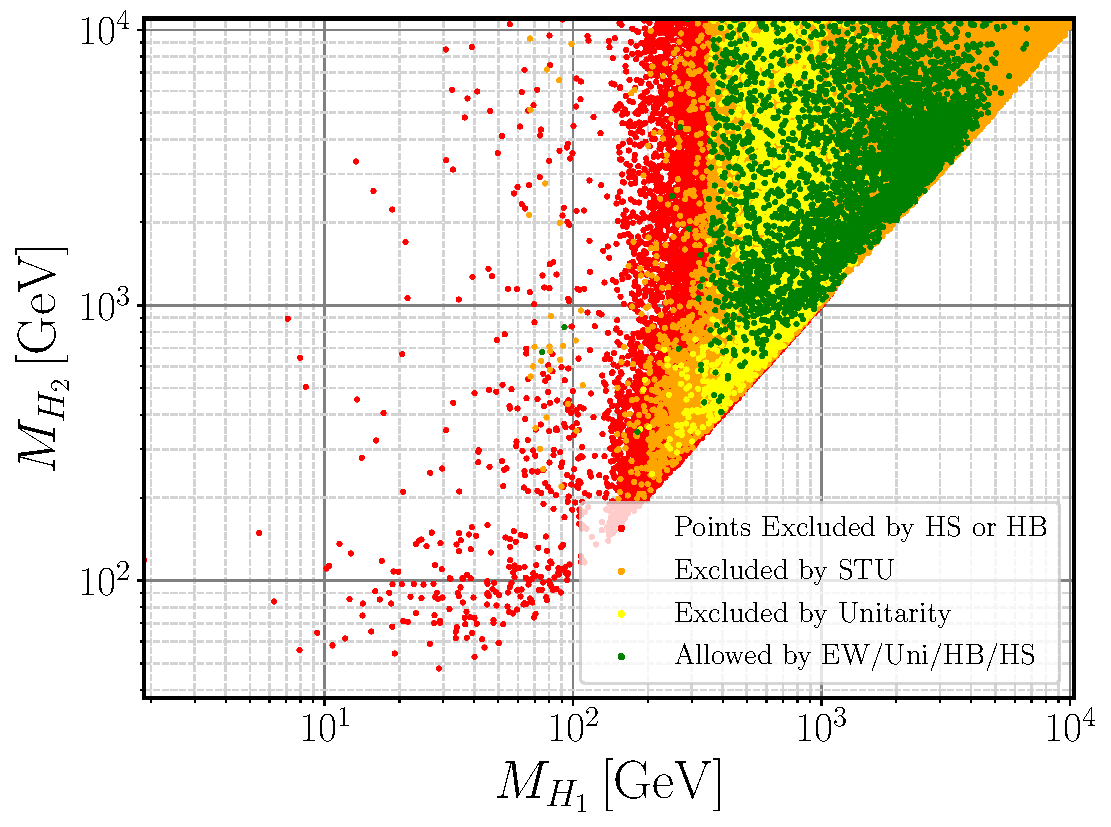
\includegraphics[width=.49\textwidth]{H1_H2_Color_Exclusions_Without_QFV.pdf}
	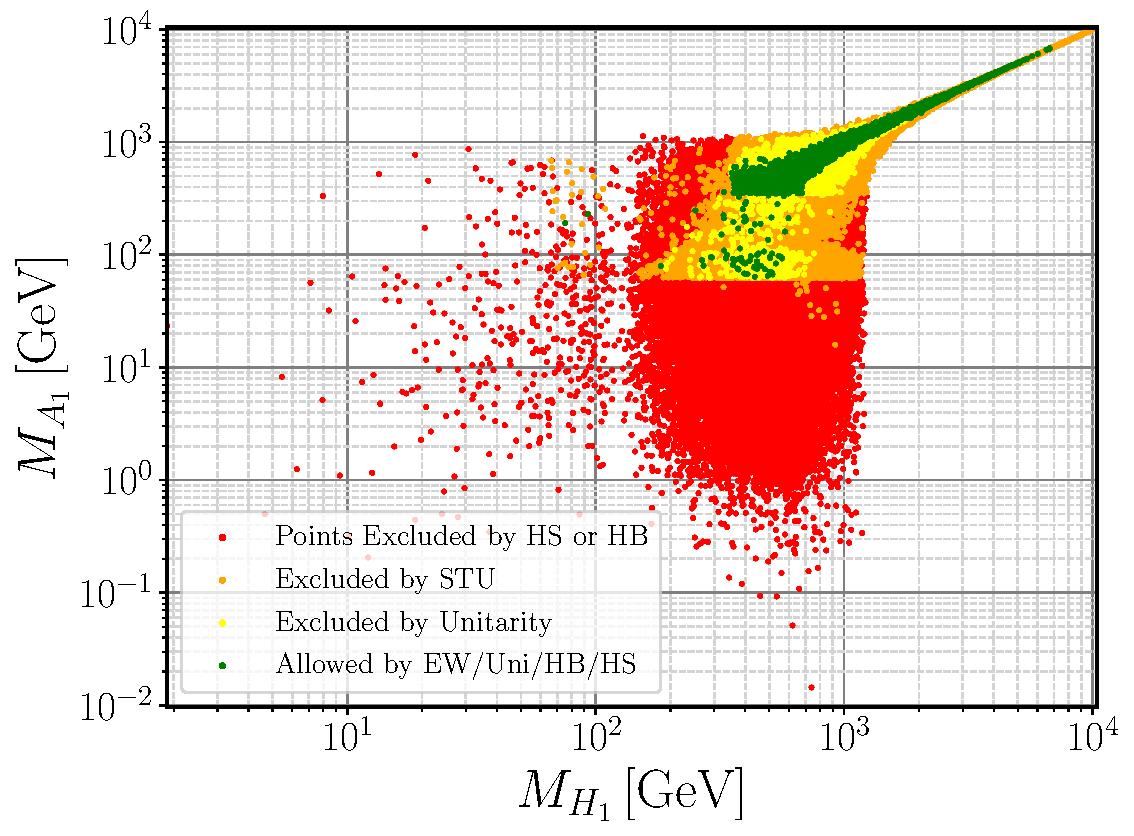
\includegraphics[width=.49\textwidth]{H1_A1_Color_Exclusions_Without_QFV.pdf}
	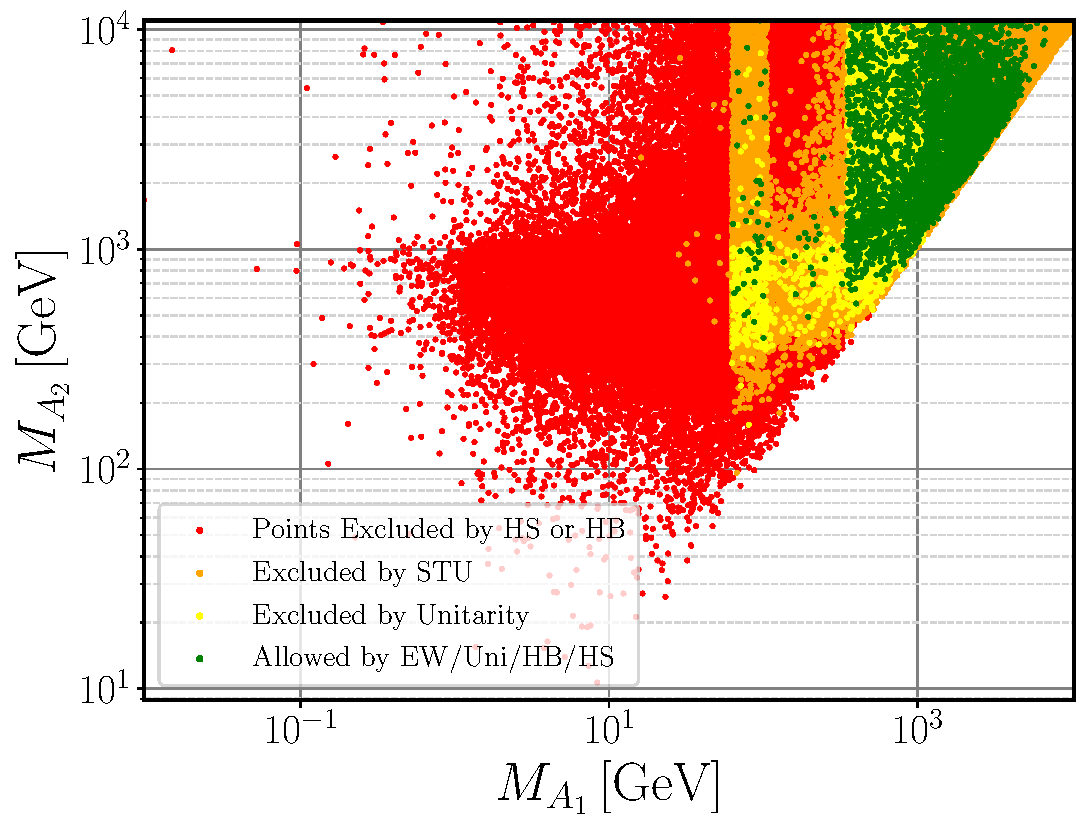
\includegraphics[width=.49\textwidth]{A1_A2_Color_Exclusions_Without_QFV.pdf}
	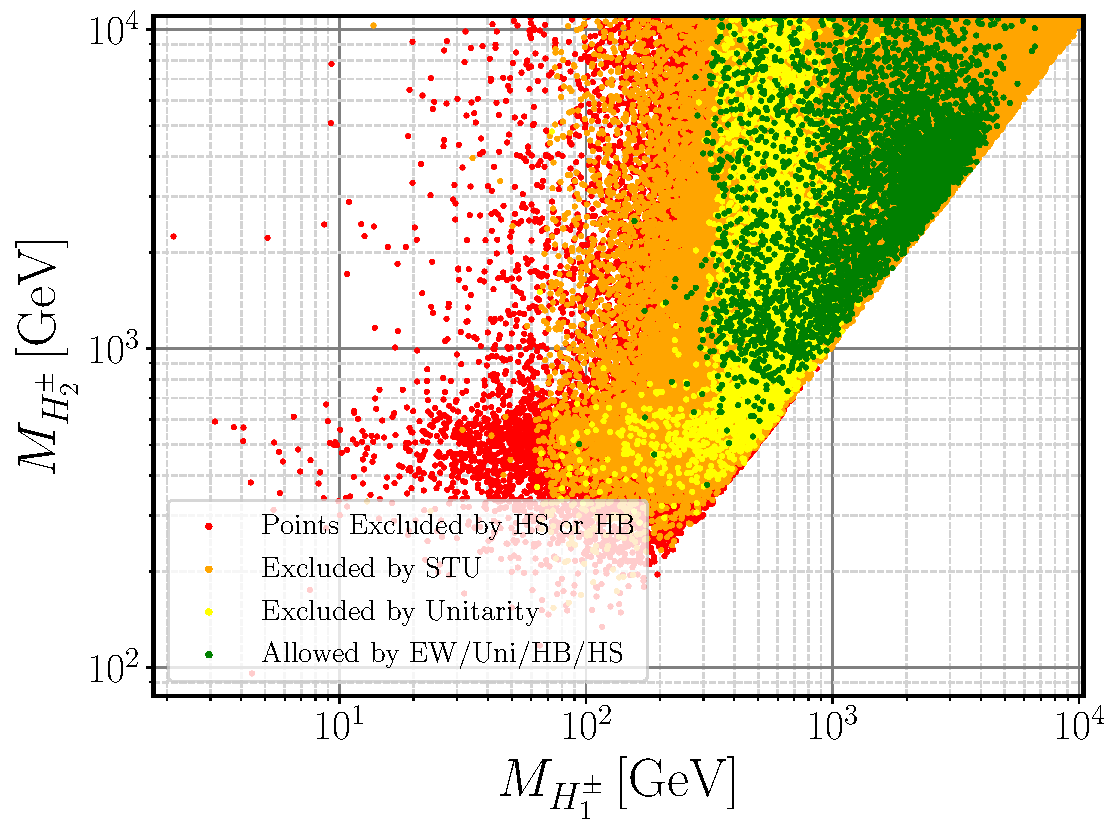
\includegraphics[width=.49\textwidth]{Hc1_Hc2_Color_Exclusions_Without_QFV.pdf}
	\label{fig:H1_A1_Plots}
\end{figure}
\end{column}    
\begin{column}{0.3\textwidth}
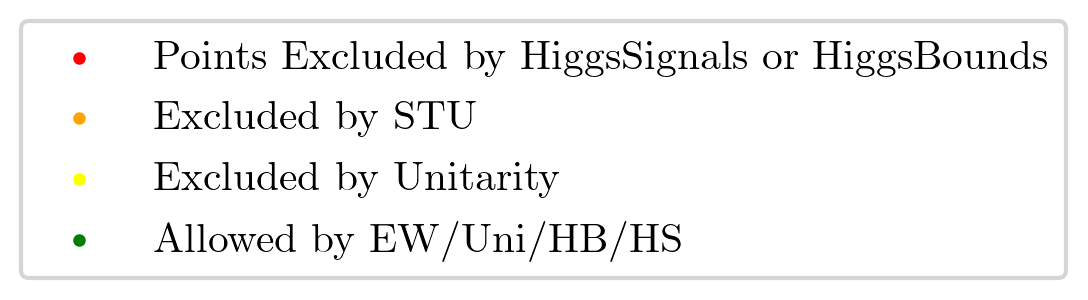
\includegraphics[width=\textwidth,origin=c,keepaspectratio]{legend1-01.png}
\end{column}    

\end{columns}

\note[item]{In red: We have points that failed HB or HS. In orange: We have points that did not survive the STU oblique paramater check. In yellow: We have points that did not survive the unitarity constraints. In green: We have points that passed all constraints up to now.  }
\note[item]{We can observe that direct searches tightly constrain the lightest pseudoscalar and scalar masses.
%
This can be seen on the red regions where, the points that failed HiggsBounds and HiggsSignals are shown. 
%
In particular, we can see that light scalars with masses bellow approximately 60 GeV are ruled out by direct searches. This essentially due to the fact that, for scalars lighter than 125 GeV ($\approx 2 \times 62.5$ GeV) Higgs decays to such scalars becomes kinematically allowed.} 
%
\note[item]{ Note that, in the bottom-left panel of Fig. when the lightest $\mathcal{CP}$-odd scalar approaches the Higgs boson mass the exclusion from direct searches becomes significantly weaker unless the second pseudo scalar also becomes lighter than 200 GeV.} 

\note[item]{
On the bottom right panel in Fig.\,\ref{fig:H1_A1_Plots} we see that STU limits and unitarity constraints also put strong constraints on how light charged scalars can be. 
%
the most dense region lies beyond 400 GeV.}
\end{frame}

\begin{comment}
\begin{frame}{3HDM - Data analysis}{Masses}
\begin{columns}
    \begin{column}{0.49\textwidth}
        \begin{figure}[!htb]
    	\centering
    	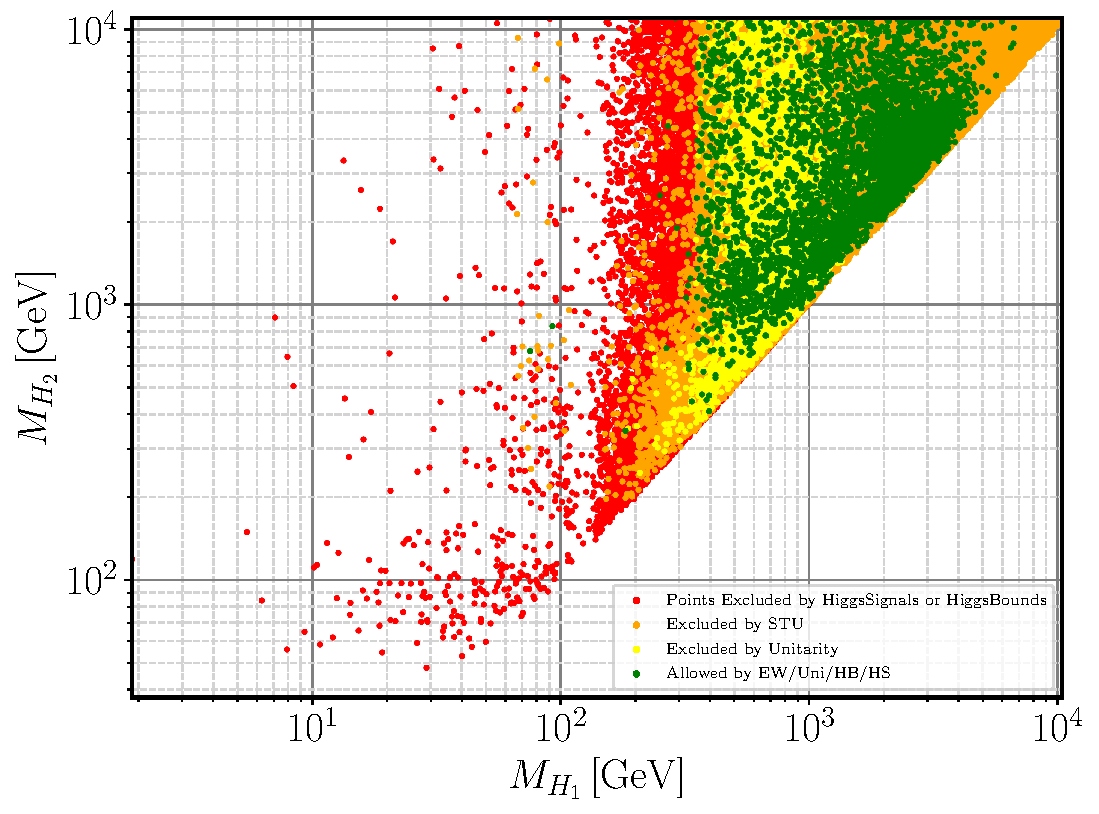
\includegraphics[width=0.8\textwidth]{/3HDM/H1_H2.pdf}
    	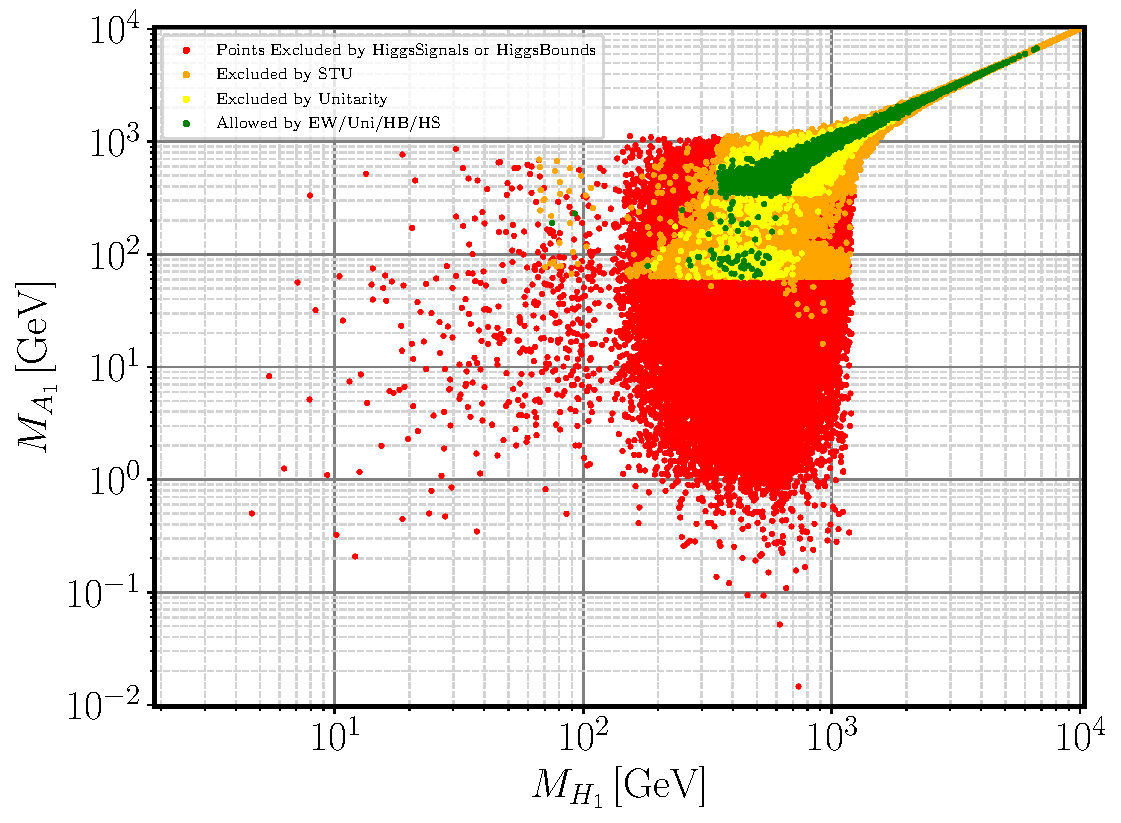
\includegraphics[width=0.8\textwidth]{/3HDM/H1_A1.pdf}
    	\end{figure}
    \end{column}
    \begin{column}{0.49\textwidth}
        \begin{center}
            {\bf Looking at the neutral scalar projections we can see that:}
        \end{center}
        \begin{itemize}
        \item The points bellow $\approx 62 \mathrm{GeV}$ are all excluded by HB and HS. This is because the Higgs boson would kinetically decay into these scalars. 
        \item On top of this we can see that STU tests also narrow down the available space not allowing scalars and pseudoscalars to differ wildly in mass scale with the exception of a region around the $100 \mathrm{GeV}$. 
    \end{itemize}
    \end{column}
\end{columns}

\end{frame} 

\begin{frame}{3HDM - Data analysis}{Masses}
\begin{columns}
    \begin{column}{0.49\textwidth}
        \begin{figure}[!htb]
    	\centering
    	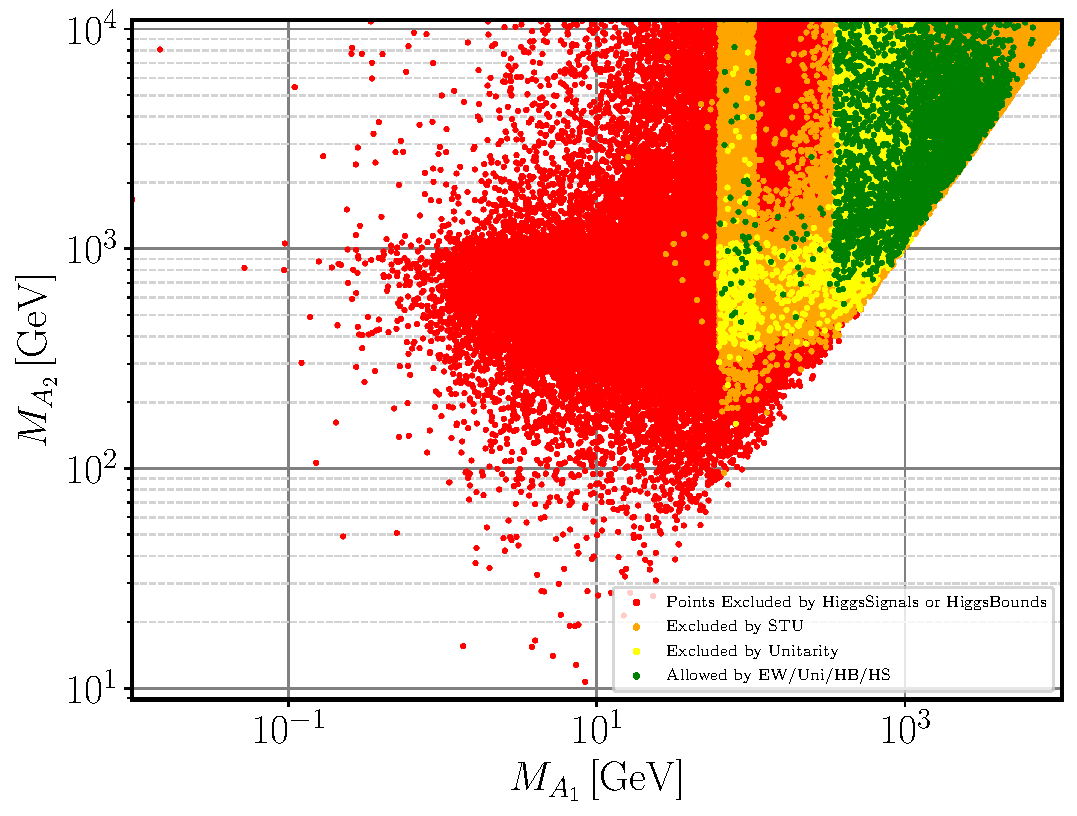
\includegraphics[width=0.8\textwidth]{/3HDM/A1_A2.pdf}
    	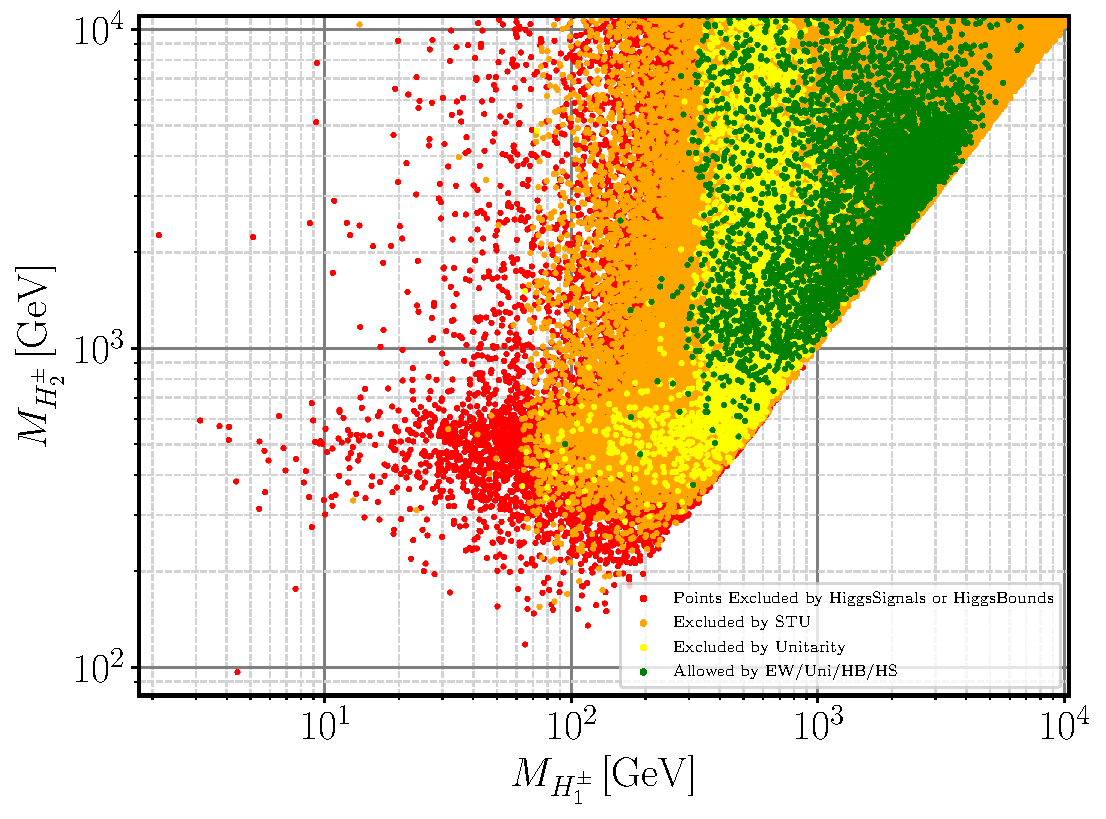
\includegraphics[width=0.8\textwidth]{/3HDM/Hc1_Hc2.pdf}
    	\end{figure}
    \end{column}
    \begin{column}{0.49\textwidth}
        \begin{center}
            {\bf Looking at the neutral scalar projections we can see that:}
        \end{center}
        \begin{itemize}
        \item The points bellow $\approx 62 \mathrm{GeV}$ are all excluded by HB and HS. This is because the Higgs boson would kinetically decay into these scalars. 
        \item On top of this we can see that STU tests also narrow down the available space not allowing scalars and pseudoscalars to differ wildly in mass scale with the exception of a region around the $100 \mathrm{GeV}$. 
    \end{itemize}
    \end{column}
\end{columns}

\end{frame} 

\end{comment}

\begin{frame}{3HDM - Data analysis}{Combination}

\begin{center}
{\bf The combination of flavour and direct measurements shows the significance of the BGL-like treatment. Direct detection creates a central region in all observables.   }
\end{center}

    \setlength{\tabcolsep}{6pt} % Default value: 6pt
\renewcommand{\arraystretch}{1} % Default value: 1

	\centering
	\begin{minipage}[t]{.32\textwidth}
	\centering
	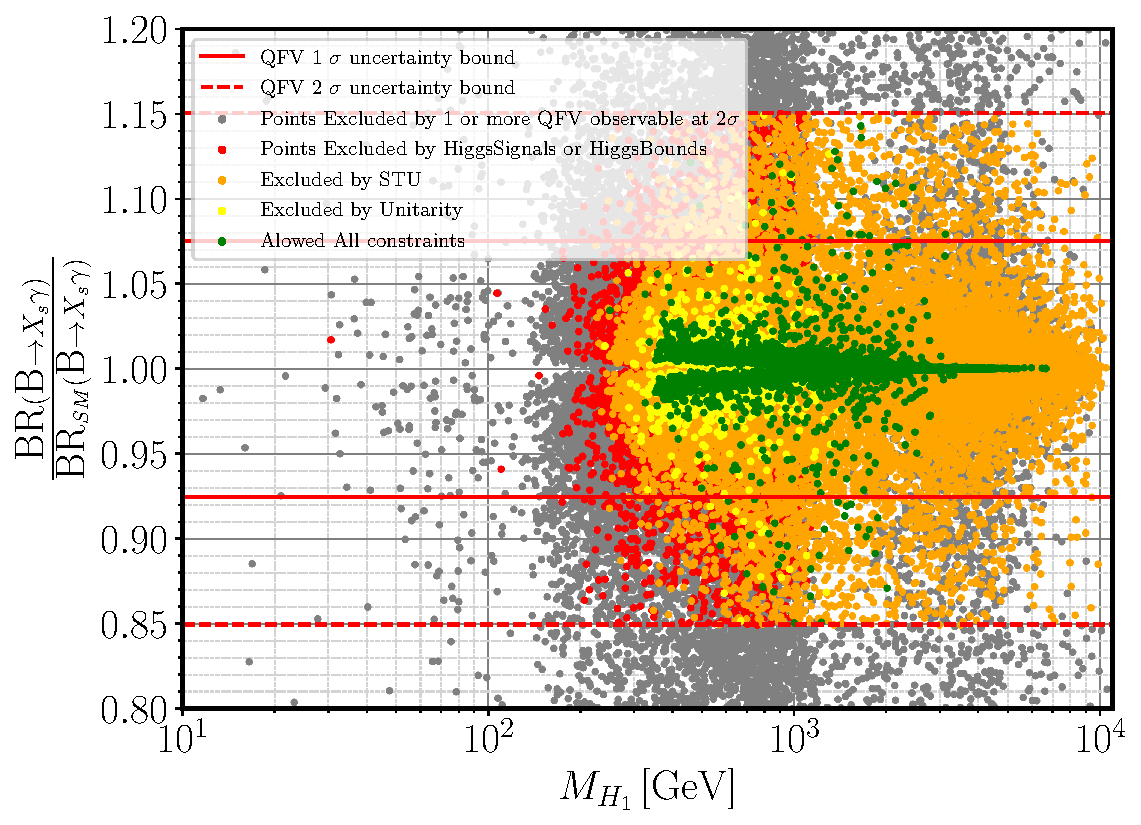
\includegraphics[width=\textwidth]{Images/3HDM/PT_Folder/XsGamma_H1.pdf}  
	\end{minipage}
	\begin{minipage}[t]{.32\textwidth}
	\centering
	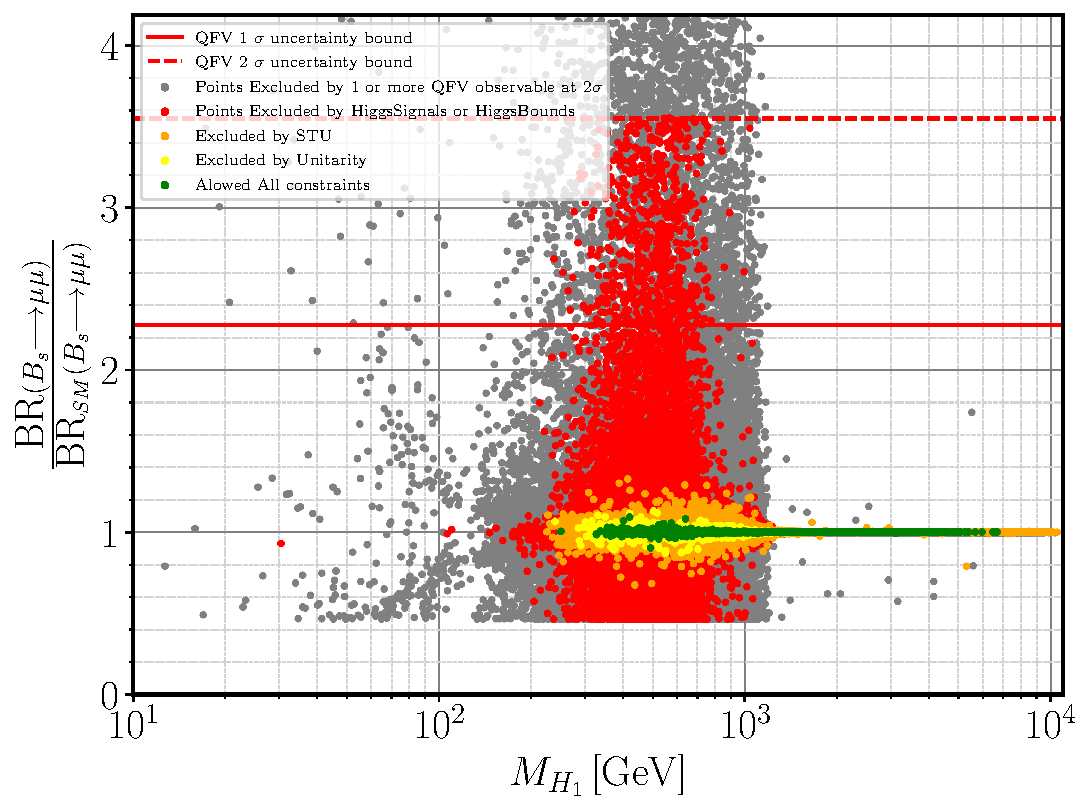
\includegraphics[width=\textwidth]{Images/3HDM/PT_Folder/Bsmumu_H1.pdf}   
	\end{minipage}
	\begin{minipage}[t]{.32\textwidth}
	\centering
	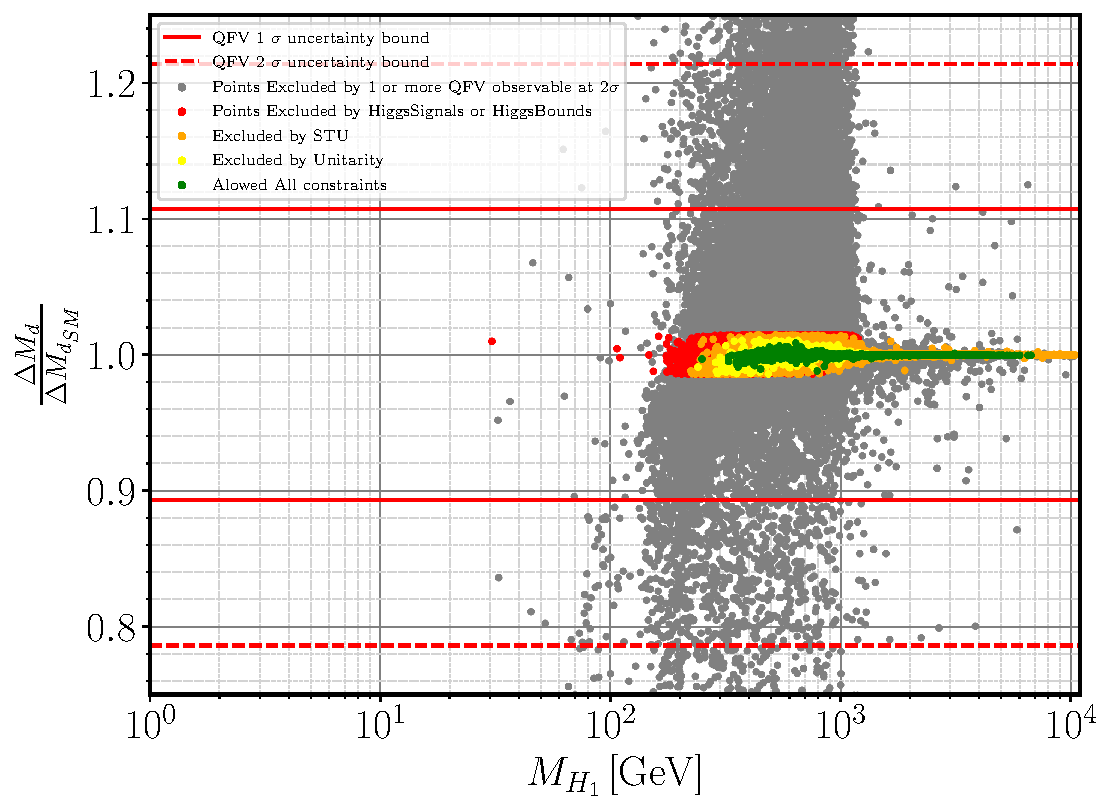
\includegraphics[width=\textwidth]{Images/3HDM/PT_Folder/Delta_Md_H1.pdf}
	\end{minipage}
	\begin{minipage}[t]{.32\textwidth}
	\centering
	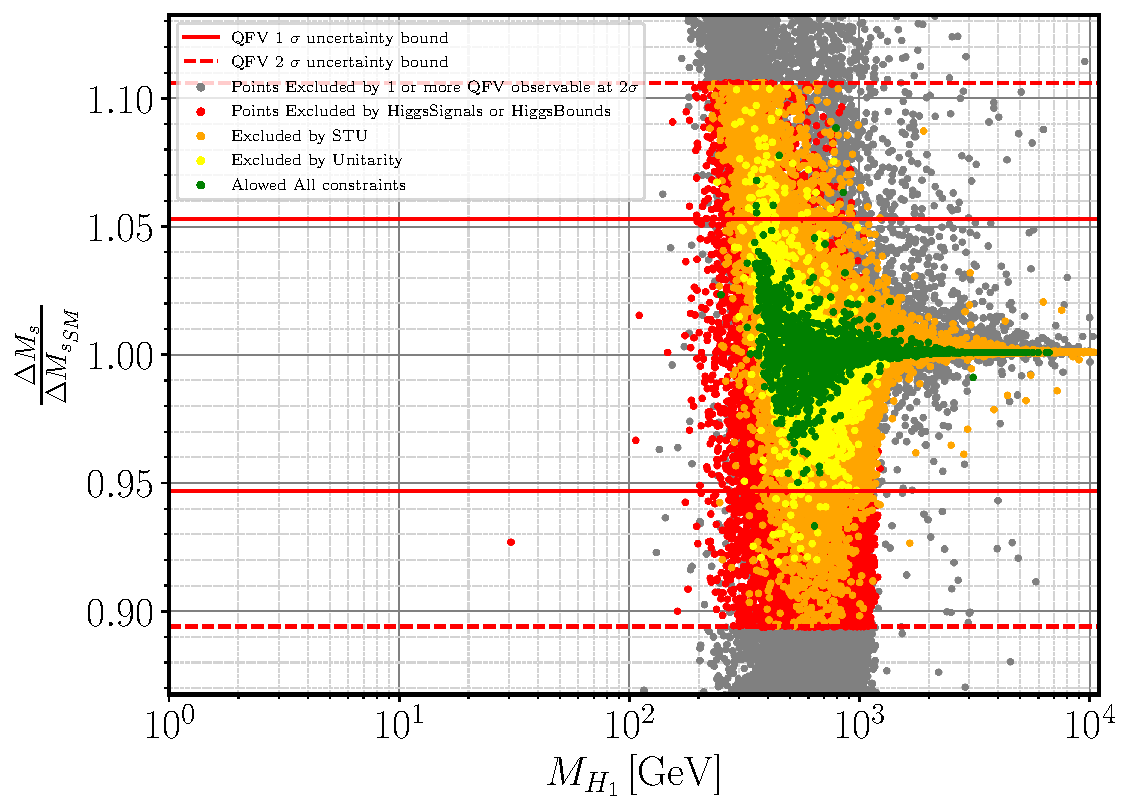
\includegraphics[width=\textwidth]{Images/3HDM/PT_Folder/Delta_Ms_H1.pdf}
	\end{minipage}
	\begin{minipage}[t]{.32\textwidth}
	\centering
	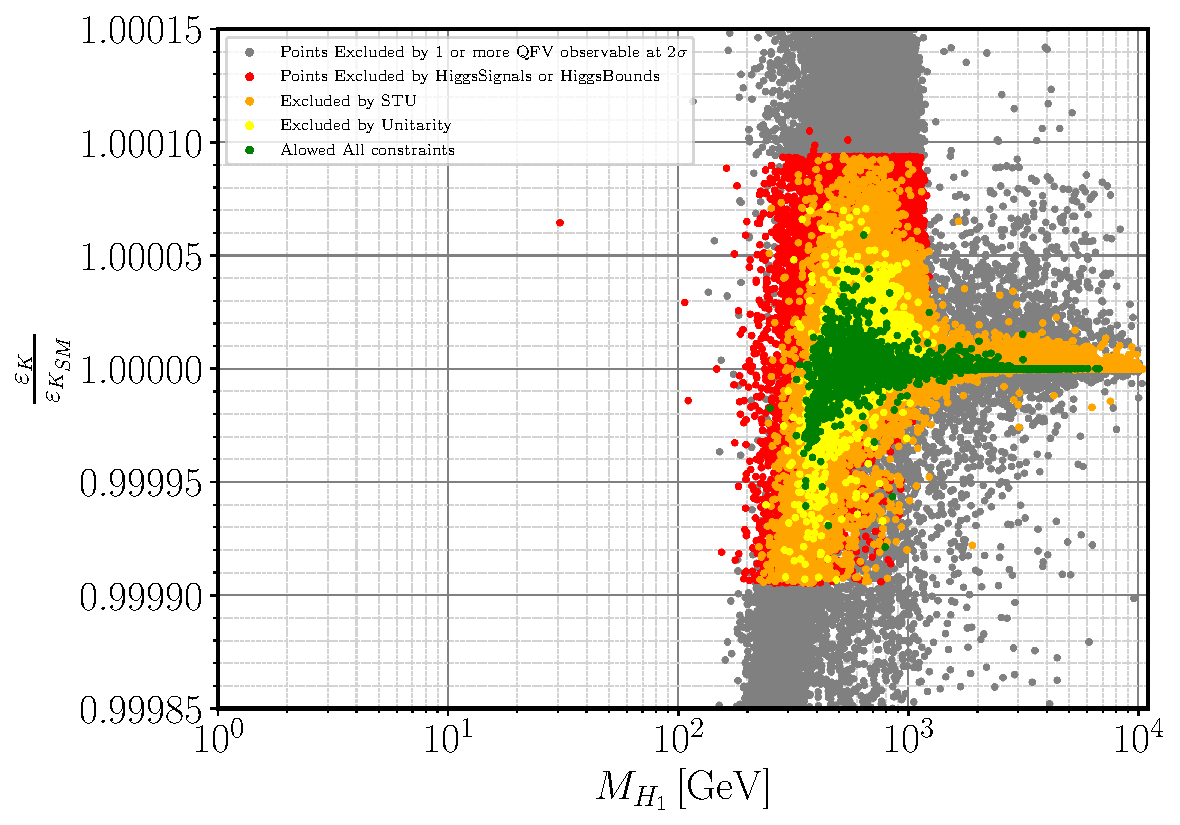
\includegraphics[width=\textwidth]{Images/3HDM/Reds/Eps_K_H1_Thighter_Centered.pdf}
	\end{minipage}
	\begin{minipage}[t]{.32\textwidth}
	\centering
	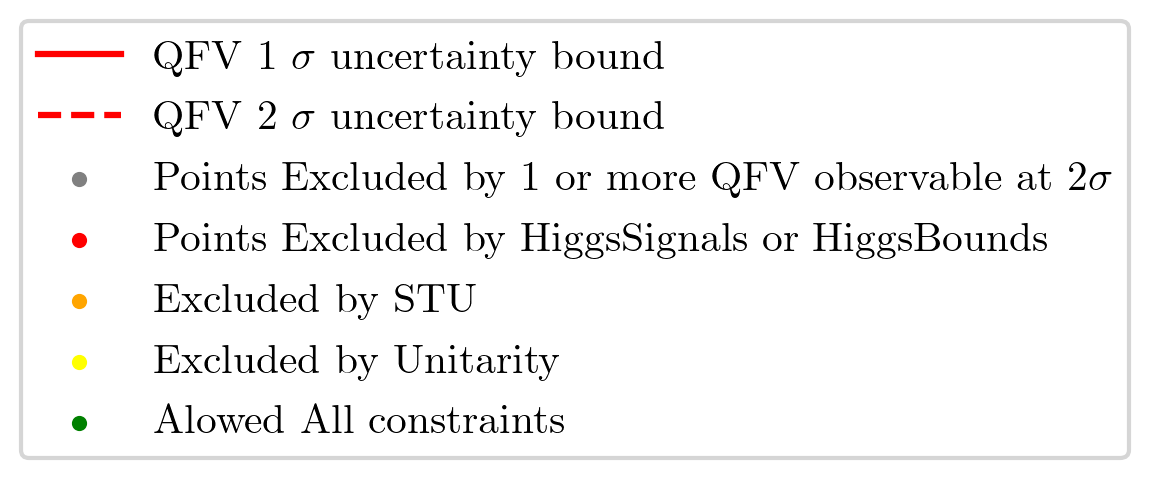
\includegraphics[width=\textwidth]{legend2-01.png} 
	\end{minipage}

	%\caption{ Scatter plot of the estimated QFV observables normalized to SM values overlapped all other experimental and theoretical constraints.} 

\note[item]{\large In particular, it is interesting to note that the green points that have also survived STU, unitarity and direct searches constraints, tend to pile close to the center of the cloud of points instead of randomly scatter. This suggests that the BGL suppression is more effective for scenarios that are consistent with such theoretical and experimental constraints.}
\note[item]{\large This is a very important conclusion we take from our model. Through the stabilization of the 3HDM by the flavour symmetry all QFV observables are kept under significant deviation for all the viable mass spectrum.  }
\note[item]{Here we see the most significant quark flavour observables in our model}
\note[item]{The first thing to highlight is that the allowed region for $\varepsilon_K/\varepsilon_{K_{SM}}$ and ${\Delta M_s}/{\Delta M_{s_{SM}} }$ appears to be rather small. This follows from the fact that the ${\textrm{BR} ( \textrm{B} \rightarrow X_s \gamma)}/{\textrm{BR}_{SM} ( \textrm{B} \rightarrow X_s \gamma )}$ and ${\Delta M_s}/{\Delta M_{s_{SM}} }$ observables are very tightly constrained and are the most sensitive ones. }
\note[item]{Note also, when we combine all QFV observables, the model prediction for the allowed region in the $\Delta M_d$ and $\epsilon_k$, red points, lies well bellow their 1 $\sigma$ uncertainty and very close to the SM value.  }
\end{frame}

    \setlength{\tabcolsep}{6pt} % Default value: 6pt
\renewcommand{\arraystretch}{1} % Default value: 1

\begin{frame}{3HDM - Data analysis}{Fine-Tuning}
\begin{columns}
    \begin{column}{0.48\textwidth}
    \begin{figure}[htb!]
    \centering
    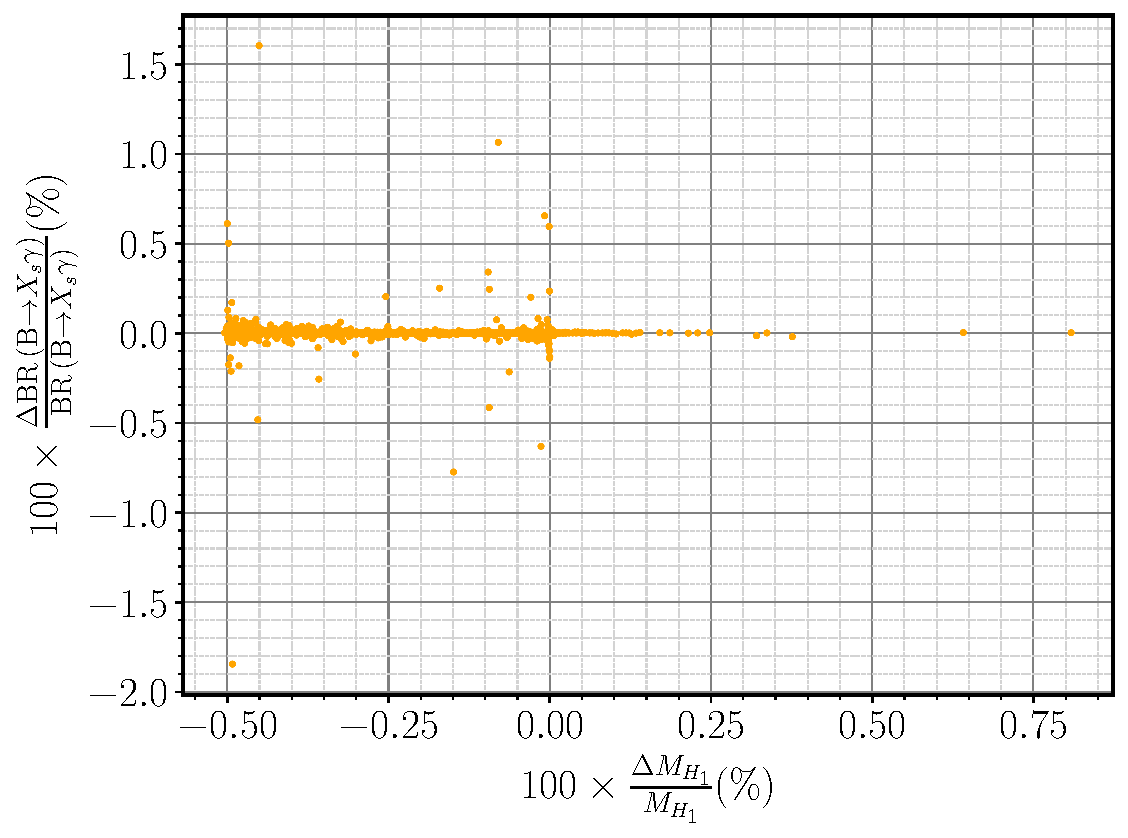
\includegraphics[width=.8\textwidth]{Images/3HDM/Fine_Tuning/Xsgamma_H1.pdf}
    \end{figure}	
    \end{column}
    %
    \begin{column}{0.48\textwidth}
    \begin{figure}[htb!]
    \centering
    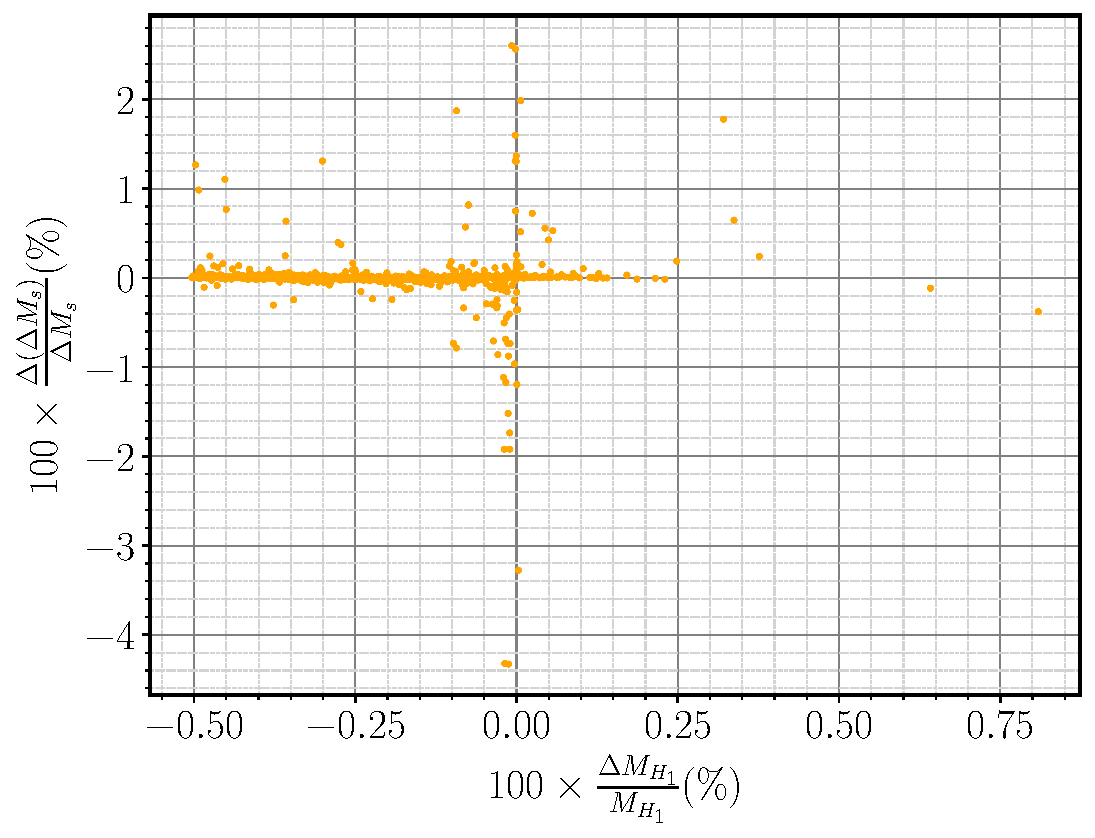
\includegraphics[width=.8\textwidth]{Images/3HDM/Fine_Tuning/DeltaMs_H1.pdf}
    \end{figure}	
    \end{column}
    
\end{columns} 

\begin{columns}
    
    \begin{column}{0.48\textwidth}
    \begin{figure}[htb!]
    \centering
    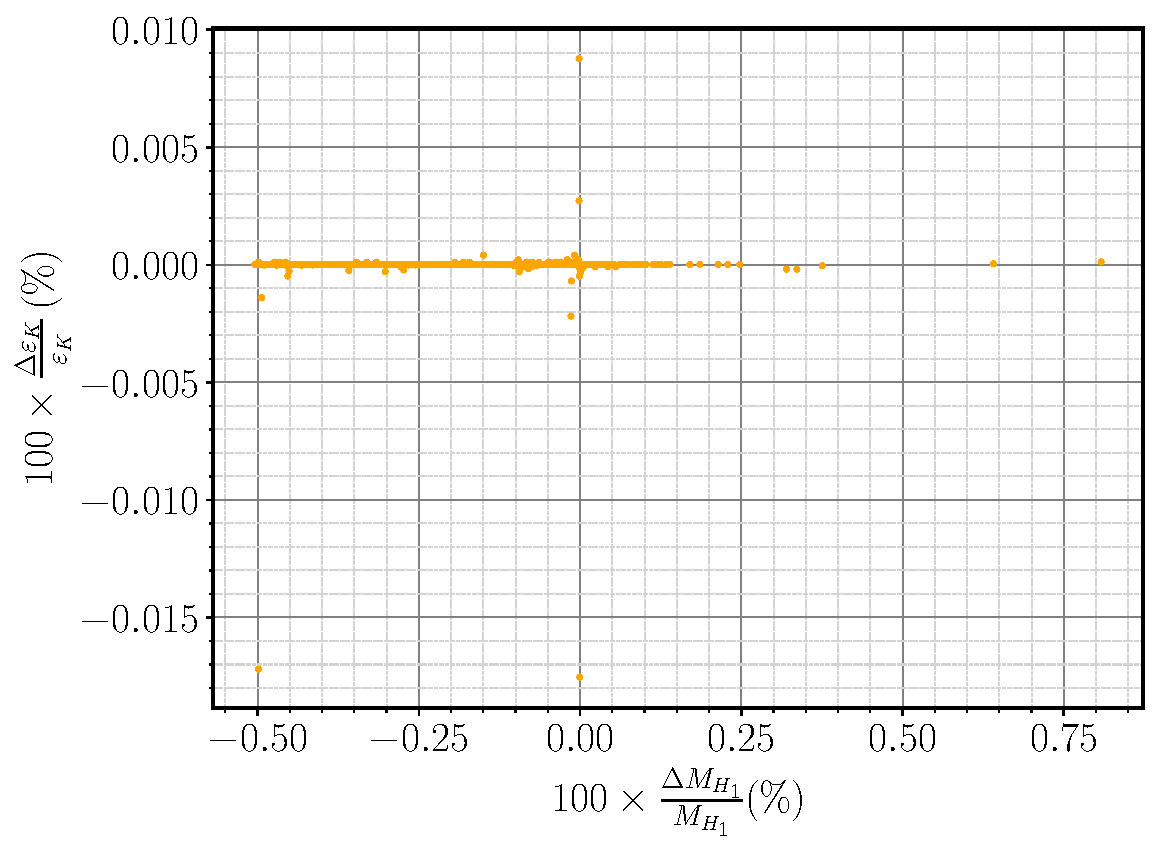
\includegraphics[width=.8\textwidth]{Images/3HDM/Fine_Tuning/eps_K_H1.pdf}
    \end{figure}	
    \end{column}
    %
    \begin{column}{0.48\textwidth}
    {\bf A complementary analysis was made where mass tuned through a 1\% change on the soft breaking terms, $\mu_{13}$, $\mu_{23}$ and $\mu_{21}$. }
    %\begin{itemize}
    %    \item No significant variation of flavour observables. Suppression is due to the flavour symmetry imposed not fine-tuning. 
    %\end{itemize}
    \end{column}

\end{columns} 
\note[item]{\large What usually is done is this model is a fine tuning of contributions to fcncs as to allow for consistency with observations. To check if this phenomena was present, all points were recalculated with a slight variation of masses through a 1\% change on the soft breaking terms, $\mu_{13}$, $\mu_{23}$ and $\mu_{21}$. 
%
Such a mass variation is expected to lead to variation of the flavour decay amplitudes. 
%
With this exercise we expect to show that there is no abruptly large variation of masses or QFV observables as to show no fine-tuning is present.}
\end{frame}

\begin{frame}{3HDM - Data analysis}{Cross section of direct production}
\begin{columns}
    \begin{column}{0.48\textwidth}
    \begin{figure}[htb!]
    \centering
    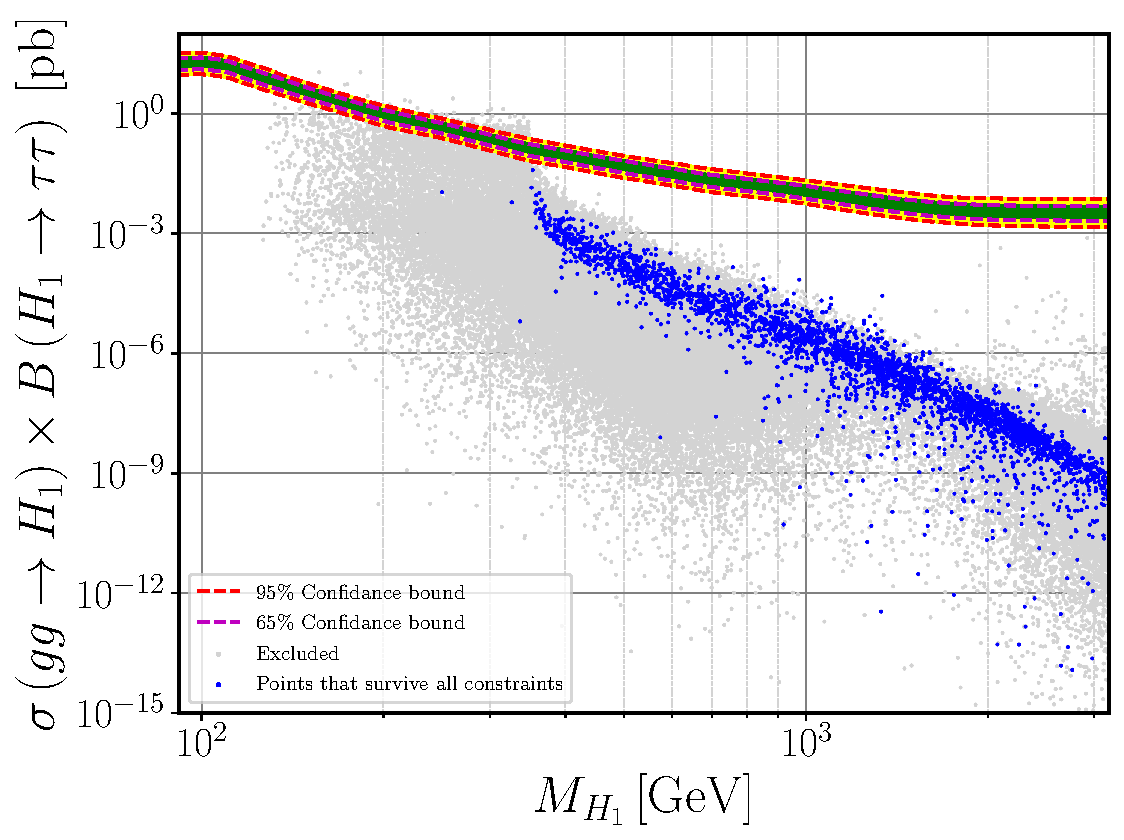
\includegraphics[width=.8\textwidth]{Images/3HDM/Xsec/Xsec_1_Grey_tight.pdf}
    \end{figure}	
    \end{column}
    %
    \begin{column}{0.48\textwidth}
    \begin{figure}[htb!]
    \centering
    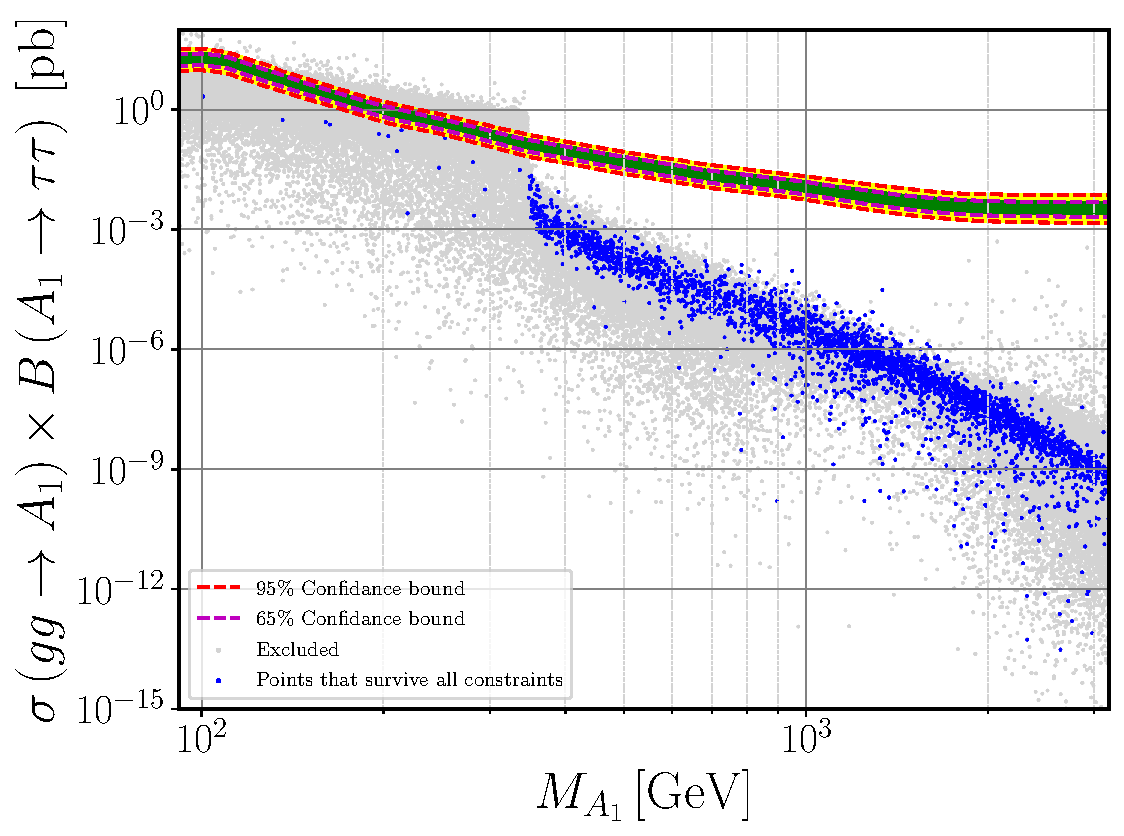
\includegraphics[width=.8\textwidth]{Images/3HDM/Xsec/Xsec_2_Colourful_tight.pdf}
    \end{figure}	
    \end{column}
    
\end{columns} 

\begin{columns}
    
    \begin{column}{0.49\textwidth}
    \begin{figure}[htb!]
    \centering
    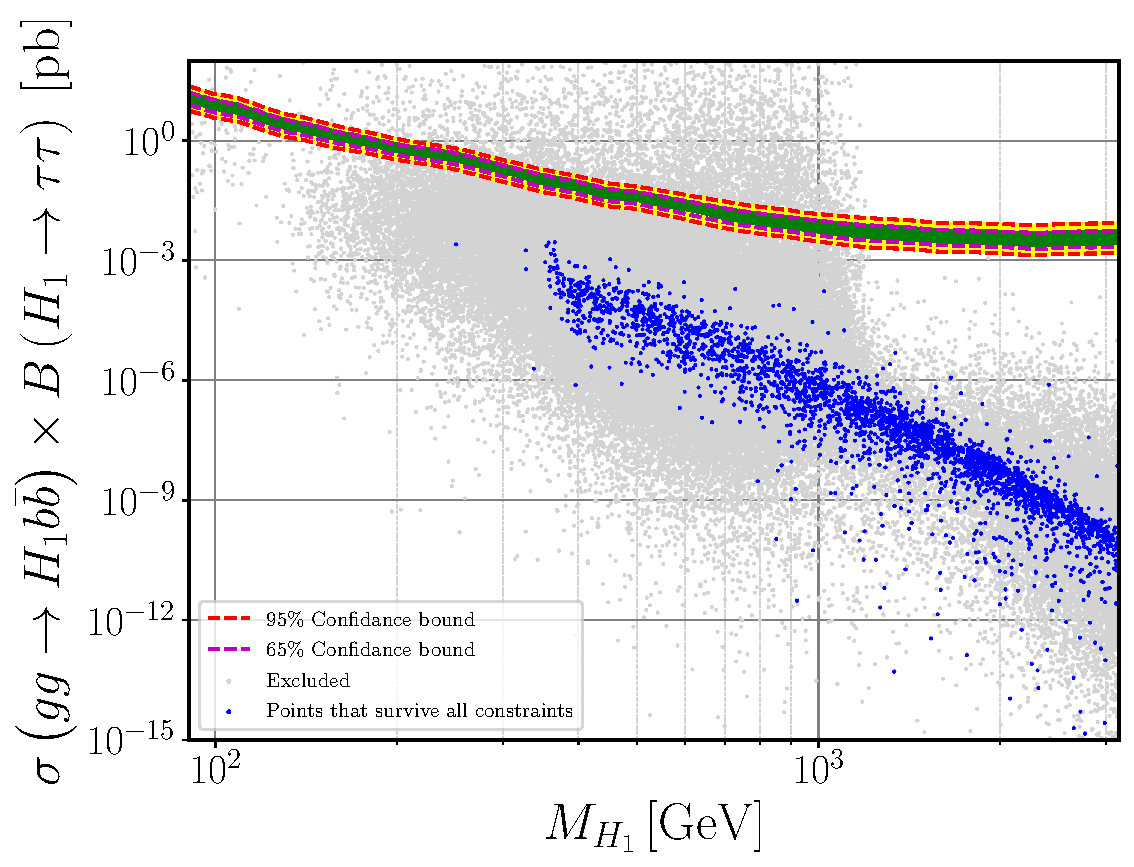
\includegraphics[width=.8\textwidth]{Images/3HDM/Xsec/Xsec_3_Grey_Thight.pdf}
    \end{figure}	
    \end{column}
    %
    \begin{column}{0.49\textwidth}
    \vskip2mm
    \begin{itemize}
        \item QFV observables lie always within allowed region of the LHC. Showing that these points can be probed in LHC III run.
    %    \item This Re-emphasizes that the 3HDM is well within reach to be probed at the LHC III upgrade. 
    \end{itemize}
    \end{column}
    \note[item]{All EW-consistent points are tested for the $\tau$ decay channel through gluon fusion into neutral scalars.}
\end{columns} 
\note[item]{\Large What we see that the QFV observables always are within the allowed region of current LHC bounds, meaning QFV is actually a stronger exclusion than direct tau decay channel for heavy scalars in our mode.}
\end{frame}

\begin{frame}{3HDM - Data analysis}{Bench-marks of the 3HDM model}
    \begin{table}[!htb]
	\centering
	\begin{tabular}{c|c|c|c|c|c|c|}
		\cline{2-7} 
		& $m_{H_1}$ & $m_{H_2}$ & $m_{A_1}$ & $m_{A_2}$ & $m_{H^\pm_1}$ & $m_{H^\pm_2}$ \\ \hline
		\multicolumn{1}{|l|}{  Second lightest $H_1$ } & 327 & 1528 & 359 & 1616 & 229 & 1561  \\ \hline
		\multicolumn{1}{|c|}{\multirow{2}{*}{Lightest $A_1$}}     & 386 & 452  & 87  & 467 & 189  & 466  \\ \cline{2-7} 
		\multicolumn{1}{|c|}{}                                    & 337 & 446  & 100 & 395 & 311  & 374  \\ \hline
		\multicolumn{1}{|l|}{Second Lightest $H^\pm_1$}  & 398 & 1314 & 282 & 1525 & 173 & 1314 \\ \hline
	    \multicolumn{1}{|l|}{Lightest $H^\pm_1$ and $H_1$}    & 251 & 2488 & 247 & 2616 & 157 & 2510  \\ \hline
		
	\end{tabular}
	\label{Tab:BadTable}
\end{table}
	\begin{itemize}
	    \item A selection of five benchmark points. All masses are given in GeV. 
	    \item These correspond to the lightest scalars found that respect all QFV and scalar sector constraints.
	    \item Coincidental lightest $H_1^\pm$ and $H_1$ parameter point.
	\end{itemize}
	
\note[item]{\large For completeness, we select six possible benchmark points}
%
\note[item]{\large As we can see from these values, several combinations of light scalars are still allowed in the model. This opens up the possibility for dedicated searches at the LHC which might lead us to a explaining of possible deviations in flavour physics.}
%
\note[item]{\large It is also very remarkable that to note that the lightest pseudoscalar is allowed to be lighter than the SMs Higgs boson with a mass as low as 87 GeV. }
%
\note[item]{\large Furthermore the benchmark that minimize $m_A$ push all other scalar masses down. For instance the heaviest charged and neutral are smaller than 470 GeV.}
%
\note[item]{\large We would like to point out that this is a particularly appealing scenario for the LHC run III.  }
\end{frame}


%\subsection{Conclusions}

\begin{frame}{3HDM}{Conclusions}
    \textbf{Scalar physics}
    \begin{itemize}
        \item  We have identified regions where both flavour and scalar sector physics are within experimental bounds and show that the BGL-like treatment can be successfully applied to a 3HDM model. 
        \item  We have also discussed the possibility of probing the model in the gluon fusion channel and shown QFV overlap with this exclusion. 
        \item  In particular we have observed that the BGL-like 3HDM offers the possibility for lighter than conventionally allowed non-standard scalars, at the reach of the LHC III.
    \end{itemize}
    \textbf{Flavour sector}
    \begin{itemize}
        \item Our analysis determined the most sensitive flavour violation channels. 
        \item Proved our model can replicate the SM like FCNCs within 2$\sigma$ deviations.
    \end{itemize}
\end{frame}

\appendix
\begin{frame}{Back-up slides}
    \begin{center}
        \Huge Back-up slides
    \end{center}
\end{frame}

\begin{frame}{B-L-SM - Data analysis}{STU analysis}
    \begin{figure}[!htb]
\centering
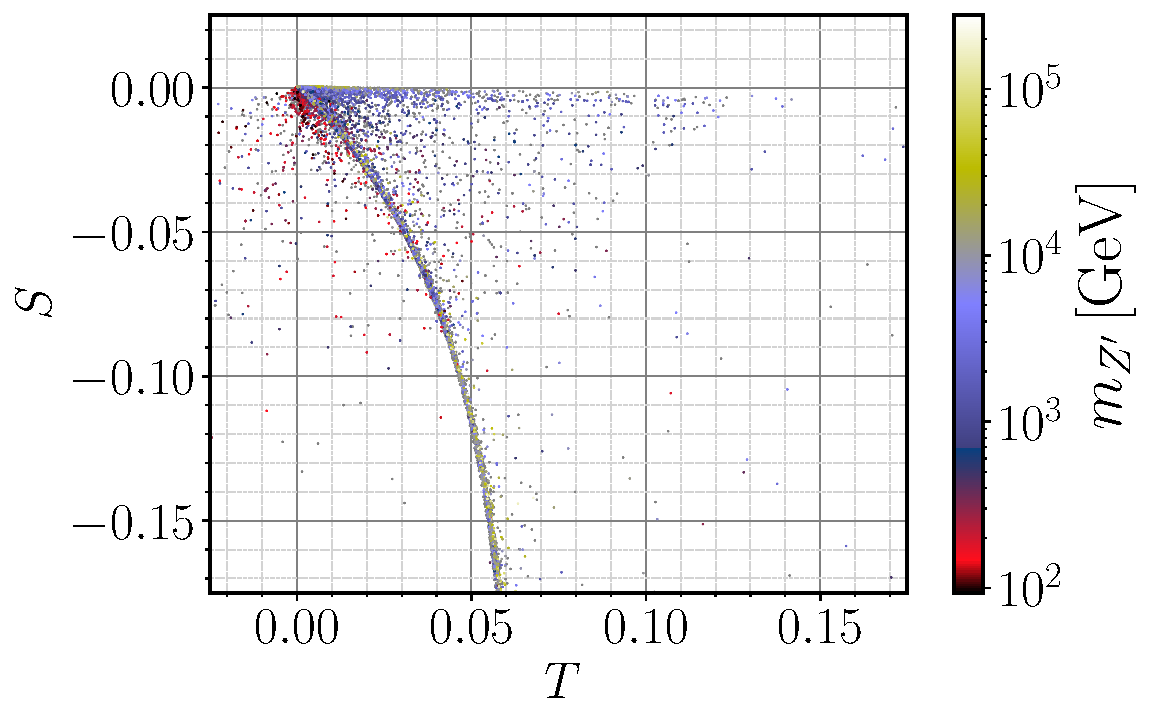
\includegraphics[width=0.35\textwidth]{Images/BLSM_2/TS_Zp.pdf}
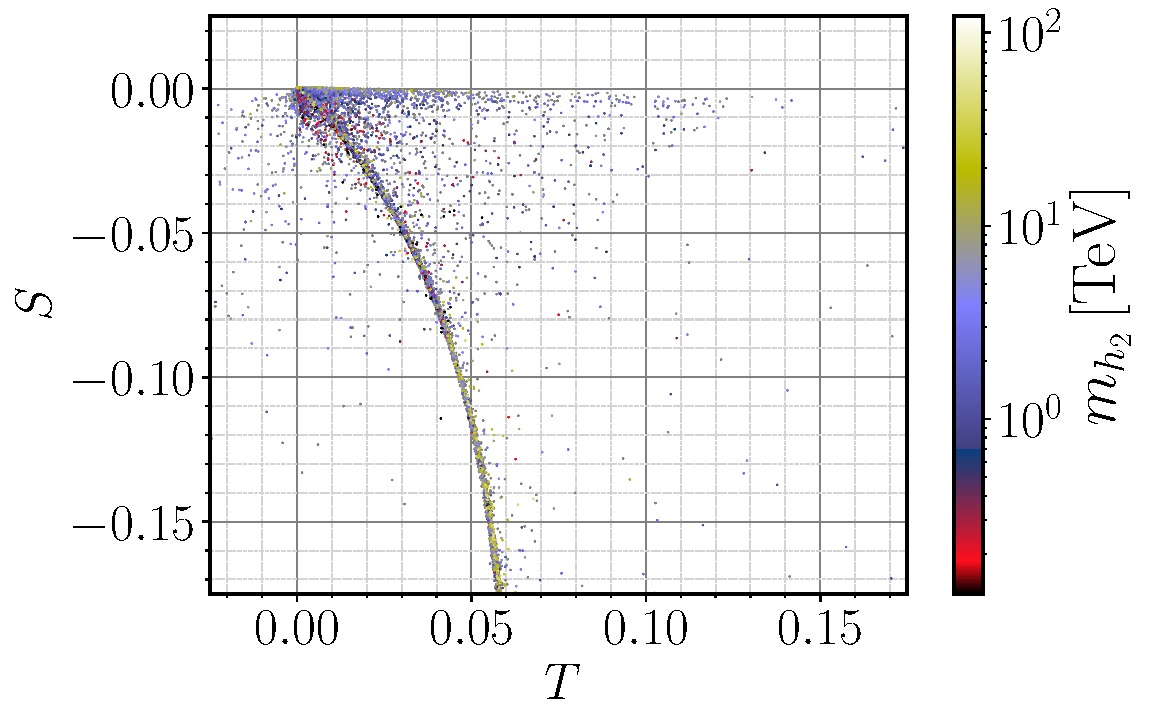
\includegraphics[width=0.35\textwidth]{Images/BLSM_2/TS_HP.pdf}
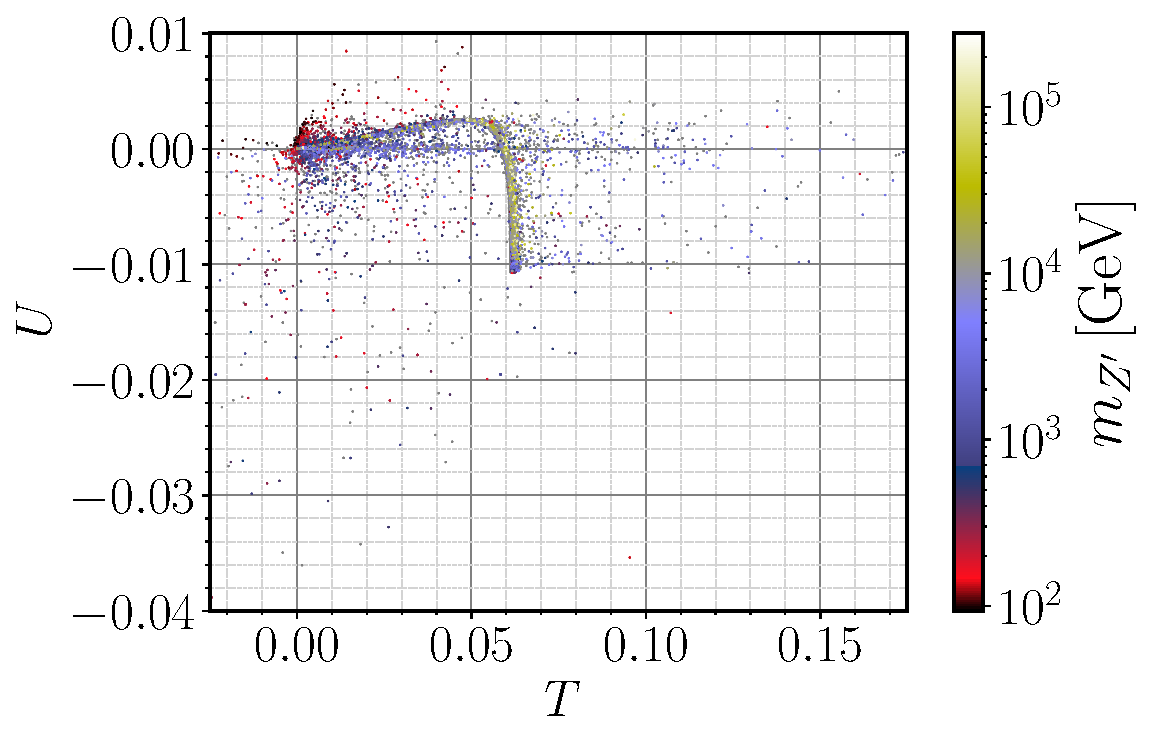
\includegraphics[width=0.35\textwidth]{Images/BLSM_2/TU_Zp.pdf}
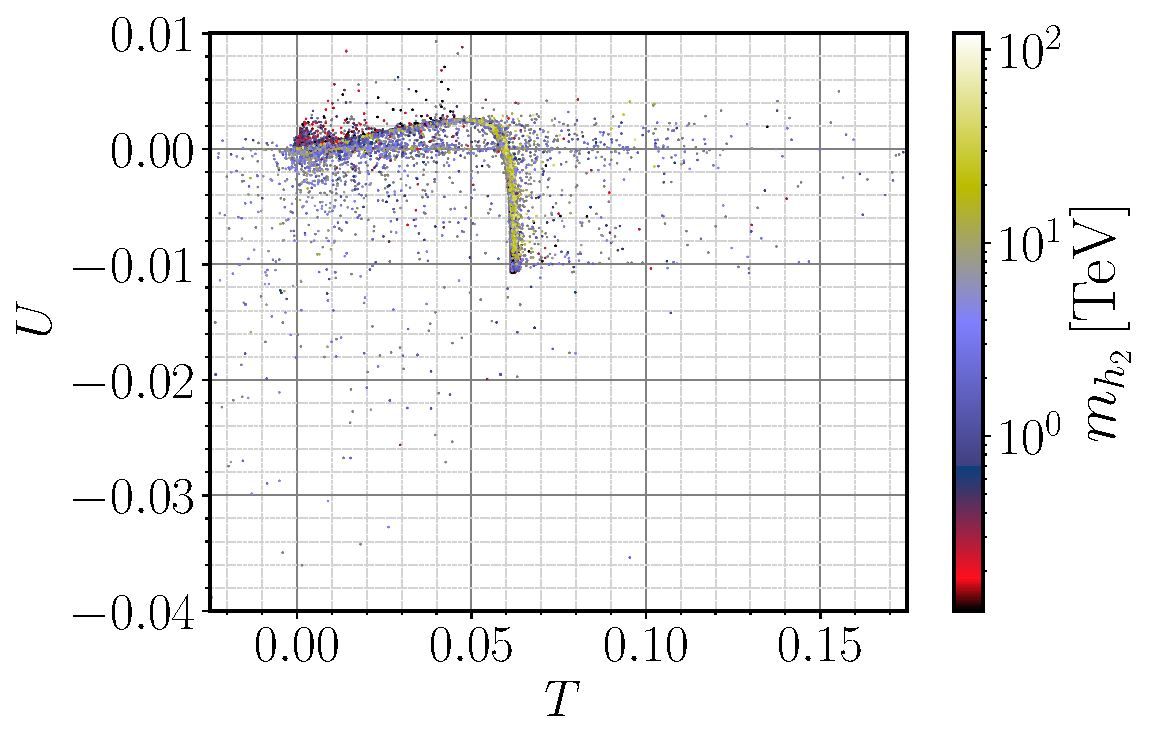
\includegraphics[width=0.35\textwidth]{Images/BLSM_2/TU_HP.pdf}
\end{figure}	

\begin{itemize}
    \item Points shown here have both:
    \begin{itemize}
        %\item Viable on scalars. 
        \item Viable scalar sector ($m_{h_1} \approx 125$ and $\chi^2$ P-value $>$ 5\%) BFB and unitarity constraint. 
        \item Within the 95\% C.L. for STU observables
    \end{itemize}
     
    \item Higher masses have a stronger effect in STU observables.
\end{itemize} 

\end{frame} 


\begin{frame}
$\Delta a_\mu^{Z^\prime}$ calculated in \texttt{SARAH} and numerically evaluated in \texttt{SPheno}
			\vskip2mm				
\begin{itemize}
	\item When $\tfrac{m_\mu}{m_{Z^\prime}} \ll 1 $ the $Z'$ contribution reads
\end{itemize}
				\begin{equation*}
				\Delta a_\mu^{Z^\prime} \approx -\tfrac{1}{3 \pi^2} \tfrac{m_\mu^2}{m_{Z^\prime}^2} \left[6 \g{L}{\mu \mu Z^\prime} \g{R}{\mu \mu Z^\prime} - 4 \left({\g{L}{\mu \mu Z^\prime}}^2 + {\g{R}{\mu \mu Z^\prime}}^2\right) \right]\,
				\end{equation*}
Contribution from $h_2$ is tiny: $\Delta a_\mu^{h_2} \propto \tfrac{m_\mu^2}{m_{h_2}^2}\left(y_\mu \sin \alpha_h\right)^2$
\vskip-2mm
%%%%%%%%%%%%%%%%%%%%%%%%%
\begin{figure}[!h]
	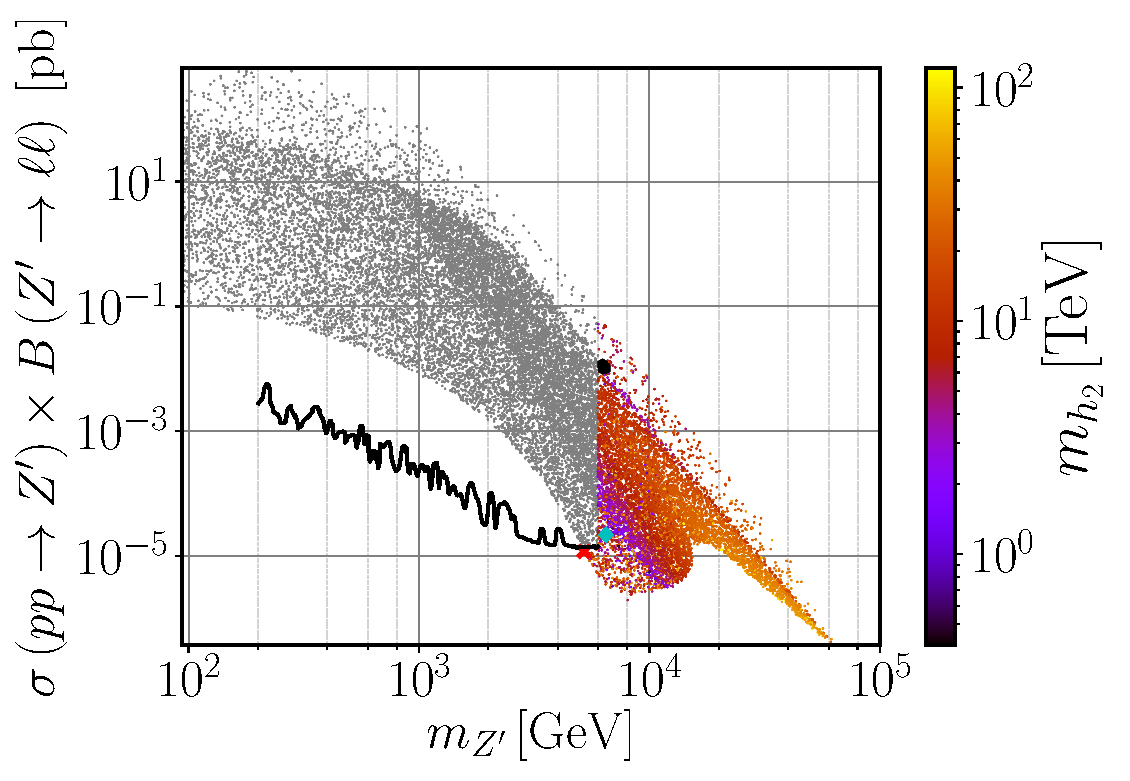
\includegraphics[width=0.45\textwidth]{Images/BLSM_2/mZp_Xsec_mh2.pdf}
	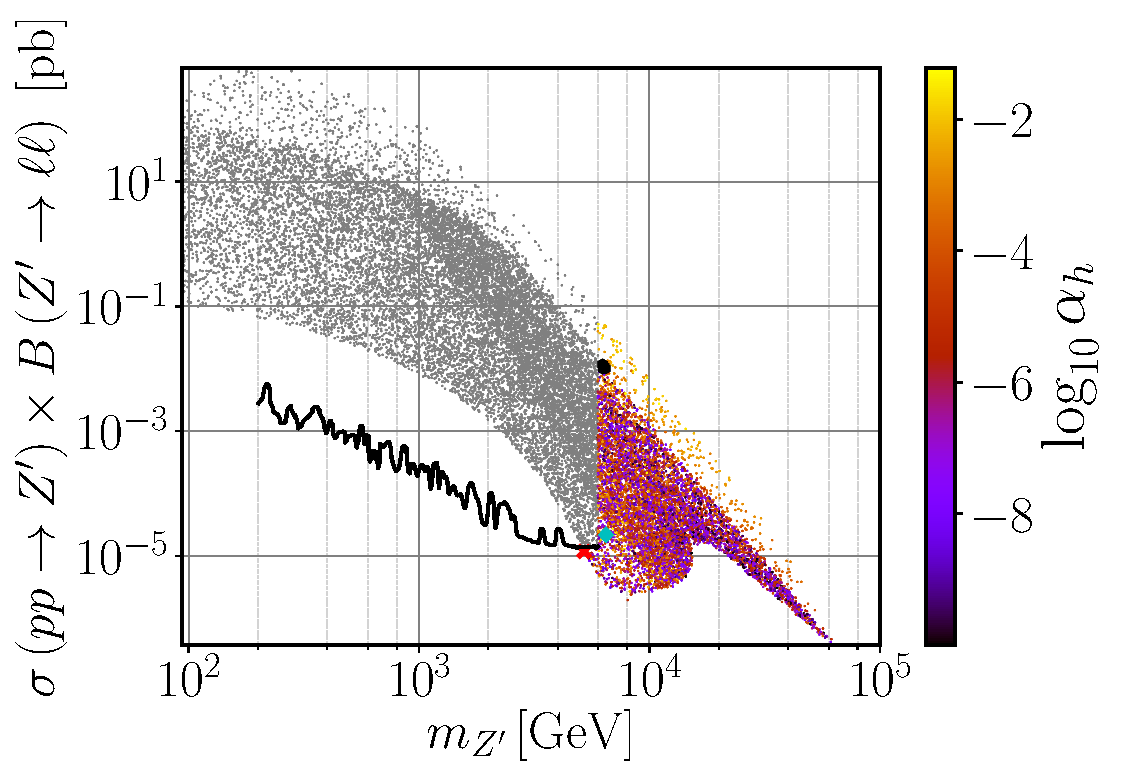
\includegraphics[width=0.45\textwidth]{Images/BLSM_2/mZp_Xsec_alpha.pdf}	
\end{figure}	
%%%%%%%%%%%%%%%%%%%%%%%%%
Suppressed by $\sin^2 \alpha_h < \mathcal{O}(10^{-2})$ and $m_{h_2} > 420~\mathrm{GeV}$
\note[item]{\Large However unlucky we must be able to explain why the (g-2) cannot be explained by our model given the points. } 
\note[item]{\Large For this let's look at the two sources of anomalous magnetic moment calculated for the Zprime and for the h2, we can see the expression for zprime here, note the as to be expected suppression by mass difference and the coupling to left and right handed muons, however we will be more interested in explaining why the h2 cannot contribute significantly.}

\note[item]{We also would like to highlight that the contribution from the new scalar is small given the angle limit and the high mass.}
\note[item]{\Large First scatter plots of the B-L-SM showing the EW oblique parameters in the $ST$ (top) and $TU$ (bot)}
\note[item]{ All coloured points here are going to be used in further analysis given they fall within the 95\% CL for STU while also having a viable Higgs with approximately 125 GeV and being within $2\sigma$ of reproducing the observed signal at the LHC. }
%\note[item]{Here we see the first points that survived the EW and Higgs direct searches made by HB and HS. }
\note[item]{Note the dependency of the masses with the EW exclusion. }
%\note[item]{The points shown here are passed the unitarity constraints in \texttt{SPheno 4.0.3} as well as the Higgs phenomenology constraints in \texttt{HiggsBounds 4.3.1} and \texttt{HiggsSignals 1.4.0}}
\end{frame}



\section{Future Work}

\begin{frame}{Future Work}{3HDM}
%\textbf{3HDM}
\begin{itemize}
    %\item A Finer analysis of the 3HDM must be made before the model is ready to be published. 
    \item Flavour effects need to be better understood. Generalized formulas for scalar couplings to quarks are missing.  
    \item A Finer look at the STU dependencies with the new scalar states needs to be better understood. 
    \item Theoretical expressions for unitarity are not written explicitly in the literature allowing us to first discovered correlations in the data. 
    %
    %\item We must look over unitarity conditions and 
    \item Computational limits exist, this model is much harder to scan than simpler models. 
    \begin{itemize}
    \item Improve the inversion process calculations by moving the C++/C, much faster. 
    \item Include machine learning to discover interesting regions much faster.
    \item Include one-loop or two-loop corrected masses in new routines.
    \end{itemize} 
\end{itemize}
\end{frame}

\begin{frame}{Future Work}{B-L-SM}
%\textbf 
\begin{itemize}
    \item The model is thoroughly examined and little parameter space remains. To provide us with more interesting physics it must be expanded. 
    \begin{itemize}
        \item The addition of a inverse seesaw-mechanism with additional neutrinos could offer more dark matter candidates. 
        \item The addition of new unitarity groups could allow the introduction of new mechanisms for anomalous momentum. 
        \item There is still the possibility of the $Z'$ being ultra-light and accounting for neutral light-interacting dark matter. 
    \end{itemize}
    \item There is still the possibility of studying this model's phase transitions as it can provide us with cosmological evidence in the form of background gravitation waves.
    \begin{itemize}
        \item This would be a good starting point to apply machine learning and to then expand on a more complex model. 
    \end{itemize}
    %
\end{itemize}
\end{frame} 

    \begin{frame}{The Standard Model}{Fields, Gauge group and Quantum Numbers}
    The \textbf{SM} is gauge Quantum Field Theory (\textbf{QFT}), that is, manifestly invariant under a set of field transformations based on the gauge group,
    \begin{equation*}
        \mathcal{G}_{SM} = \mathrm{SU}(3)_{\mathrm{C}} \times \mathrm{SU}(2)_{\mathrm{L}} \times {Y} \, .
    \end{equation*}
    %
    \begin{center}
        \textbf{Gauge, Fermion and Scalar fields and quantum numbers in the SM.} 
    \end{center}
    %
    \begin{table}[!htb]
	\centering
    	\begin{tabular}{@{}cccccc@{}}
    		\hline	
    		Fields & Spin 0 field & Spin 1 Field & $ \mathrm{ SU(3)_C \times SU(2)_L \times U(1)_Y } $  \\
    		\hline	
    		Gluons  & $\times$  & $G^a$ & (\textbf{8},\textbf{1},0) \\	
    		A bosons & $\times$  & $A^a$ & (\textbf{1},\textbf{3},0)   \\
    		B bosons & $\times$  & $B$   & (\textbf{1},\textbf{1},0)   \\
    		Higgs field & ($\phi^\pm, \phi^0 )$  & $\times$ & (\textbf{1},\textbf{2},1) \\ \hline
    	\end{tabular}
    \end{table}
    %
    \begin{table}[!htb]
	    \centering
	    \begin{tabular}{@{}cccccc@{}}
    		\hline	
    		Fields & Spin $\frac{1}{2}$ Field & $\mathrm{ SU(3)_C \times SU(2)_L \times U(1)_Y} $   \\
    		\hline	
    		Quarks (3 gen.) & $Q=(u_L,d_L)$ & $(\mathbf{3},\mathbf{2},{1}/{3})$ \\	
    		$\quad$        & $u_R$ & $(\mathbf{3},\mathbf{1},{4}/{3})$   \\
    		$\quad$   & $d_R$ & $(\mathbf{3},\mathbf{1}, -{2}/{3})$   \\
    		Leptons (3 gen.) & $L=(\nu_{e_L}, e_L )$ & $(\mathbf{1},\mathbf{2},-1)$  \\
    		$\quad$   & $e_R$ & $(\mathbf{1},\mathbf{1},-2)   $ \\ \hline
    		%
    	\end{tabular}
    \end{table}
    %
    \end{frame}
    %
    \begin{frame}{The Standard Model - Formulation}{Higgs Mechanism and Spontaneous Breaking of Symmetry}
        %
        Given the field content of the SM we can construct the Lagrangian as, 
        \begin{equation*}
            \mathcal{L}_{\text{SM}} = \mathcal{L}_{\text{kin}}  +  \mathcal{L}_{\text{Yuk}} +  \mathcal{L}_{\phi} , 
        \end{equation*}
        %
        these components are written as, 
        %
        \begin{align*}
        \mathcal{L}_{\text{kin}} = & - \frac{1}{4} G^{\mu \nu}_a G_{a \, \mu \nu}  - \frac{1}{4}  A^{\mu \nu}_a A_{a \,\mu \nu}  
        - \frac{1}{4}  B^{\mu \nu} B_{\mu \nu}  \\ 
        & -i \bar{Q}_{L_i} \slashed{D} Q_{L_i} 
        -i \bar{u}_{R_i} \slashed{D} u_{R_i}  
        -i \bar{d}_{R_i} \slashed{D} d_{R_i}  
        -i \bar{L}_{L_i} \slashed{D} L_{L_i}    
        -i \bar{e}_{R_i} \slashed{D} e_{R_i}   \\
        & - (D_\mu H)^\dagger ( D^\mu H ) ,   
        \end{align*}
        %
        \begin{equation*}
            \mathcal{L}_\phi = - \mu^2 H H^\dagger + \lambda (H H^\dagger)^2 ,
        \end{equation*}
        %
        \begin{equation*}
            \mathcal{L}_{\text{Yuk}} =  Y^u_{ij} \bar{Q}^i u_{R}^j  \tilde{H} + Y^d_{ij} \bar{Q}^i  d_{R}^j H  + Y^e_ij \bar{L}^i  e_{R_i} H + \text{H.c.} .
        \end{equation*}
        %
        {\red No explicit mass terms} but for the scalar. \textbf{All} masses are generated by the Higgs mechanism.
        %
    \end{frame}
    % ------ %
    \begin{frame}{The Standard Model - Formulation}{Higgs Mechanism and Spontaneous Breaking of symmetry}
        %
        The Higgs mechanism is characterized by the Higgs field taking on a non-zero vacuum value called the electroweak Vacuum Expectation Value (\textbf{VEV}),
        %
        \begin{equation*}
            (H^\dagger H)^2 = \frac{-\mu^2}{2\lambda} \equiv  v^2  .
        \end{equation*} 
        %
        This sets off the process of Spontaneous Symmetry Breaking (\textbf{SSB}). And breaks 3 of the SMs gauge group and it is modified to, 
        %
        \begin{equation*}
            {\mathrm{SU}(2)}\mathrm{_{L}} \times \U{Y} \rightarrow \U{Q}.  
        \end{equation*}
        %
        The generated 3 Goldstone bosons are rotated into the gauge fields, so we can write, 
        %
        \begin{equation*}
            H = \begin{pmatrix}
            \phi_1 + i \phi_2 \\ 
            v + h + i \phi_3 
            \end{pmatrix}   \rightarrow  \langle H  \rangle =  \frac{1}{\sqrt{2}} \begin{pmatrix}
            0 \\ 
            v + h 
            \end{pmatrix} \, .
        \end{equation*}
        %
    \end{frame}
    % ------ %
    \begin{frame}{The Standard Model - Formulation }{Gauge Terms and Bosons}
        %
        We can show how \textbf{square} terms now appear in the Lagrangian, all dependent on {\blue $v$}. First for the gauge bosons and the Higgs,
        %
        \begin{align*}
        \mathcal{L}_{\text{Gauge}}^\prime = & \frac{1}{2} \partial_\mu h \partial^\mu h - \frac{1}{2} (2{\blue v}^2 \lambda) h^2
        - \frac{1}{4}  A^{\mu \nu}_a A_{a \, \mu \nu}  
        - \frac{1}{4}  B^{\mu \nu} B_{\mu \nu}  \nonumber \\
        & + \frac{1}{8} {\blue v}^2 g^2 (A^1_\mu A^{1,\mu}+ A^2_\mu A^{2,\mu}) \\ & +  \frac{1}{8} {\blue v}^2  (g^2  A^3_\mu A^{3,\mu} + g^{\prime 2} B_\mu B^\mu - 2 g^2 g^{\prime 2} A^3_\mu B^\mu ) + \cdots  \ , 
        \end{align*}
        %
        From these terms we can reach the charge and mass eigenstates for the fields,
        \begin{gather*}
            W^\pm_\mu = \frac{1}{\sqrt{2}} (A^{1}_\mu \pm i A^{2}_\mu) ,  Z_\mu =- \sin(\theta_W) B_\mu + \cos(\theta_W) A_\mu^3 , \\ A_\mu =\cos(\theta_W) B_\mu + \sin(\theta_W) A_\mu^3  . 
        \end{gather*}
        From this we can see, the Higgs mass, and the following square terms, 
        %
        \begin{equation*}
        M_h= (2v^2 \lambda), \quad  
        m_{\text{Gauge}}^2 =
        \dfrac{v^2}{4}
        \begin{pmatrix}
        g^2 \;\;&\;\; 0 \;\;&\;\; 0 \;\;&\;\; 0 \;\; \\
        0 \;\;&\;\; g^2 \;\;&\;\; 0 \;\;&\;\; 0 \;\; \\
        0 \;\;&\;\; 0 \;\;&\;\; g^2 \;\;&\;\; -g g_{Y} \;\; \\
        0 \;\;&\;\; 0 \;\;&\;\; -g g_{Y} \;\;&\;\; g_{Y}^2 \;\; \\
        \end{pmatrix} , 
        \end{equation*} 
        %
        The proper charge and mass eigenstates of the gauge states, 
        %
        \begin{equation*}
            \quad M_{W^\pm}= \frac{1}{2} v g , \quad M_Z =  \frac{1}{2} v \sqrt{g^2 + g^{\prime 2}}, \quad  M_\gamma = 0 \, . 
        \end{equation*}
    \end{frame}
    % ------ %
    \begin{frame}{The Standard Model - Formulation}{Yukawa Interactions - the case for leptons}
        %
        The same can be done for fermions, where,
        %
        \begin{equation*}
        \begin{split}
            \mathcal{L}_{\text{lep.}} & = Y_e^{ij} \Phi_L^i H e_R^i + \text{H.c.}\, \\ 
            = & \frac{y_e {\blue v}}{\sqrt{2}} e_L e_R + \frac{y_\mu {\blue v}}{\sqrt{2}} \mu_L \mu_R + \frac{y_\tau {\blue v}}{\sqrt{2}} \tau_L \tau_R + \big(\text{Interactions with }h\big) + \text{H.c.} \, ,
        \end{split} 
        \end{equation*}
        %
        given, $Y_e^{ij}$, is \textbf{diagonal} we can show, 
        %
        \begin{equation*}	
            m_e = \frac{y_e {\blue v}}{\sqrt{2}} \,,\, m_\mu = \frac{y_\mu {\blue v}}{\sqrt{2}} \,,\, \ m_\tau = \frac{y_\tau {\blue v}}{\sqrt{2}} \,.
        \end{equation*} 
        %
        However, \textbf{for quarks}, where $Y_u^{ij}$ is not {\red diagonal}.
        %
        \begin{equation*}
            \mathcal{L}_{{\text{qrk.}}} = Y_d^{ij} \bar{Q}^i_L H  d_R^j + Y_u^{ij} \bar{Q}^i_L \tilde{H} u_R^j + \text{H.c.}
        \end{equation*} 
        %
        \begin{equation*}
            \mathcal{L}_{\text{qrk.}} = \frac{ Y_d^{ij} {\blue v}}{\sqrt{2}} \bar{d}_L d_R + \frac{ Y_u^{ij} {\blue v}}{\sqrt{2}} \bar{u}_L u_R + \big(\text{Interactions with }h\big) + \text{H.c.}
        \end{equation*}
        %
        To diagonalize the mass eigenstates we must perform a set of \textbf{unitary transformations} on the quark fields. Thus through the relations, 
        %
        \begin{equation*}
            \bar{d}^\prime_{L} = \bar{d}_{L} U^d_{L} \quad , \quad d^\prime_{R} = U^d_{R} \,^\dagger d_{R}  \quad , \quad
            \bar{u}^\prime_{L} = \bar{u}_{L} U^u_{L} \quad , \quad u^\prime_{R} = U^u_{R} \,^\dagger u_{R} \,. 
        \end{equation*}
        %
    \end{frame}

\begin{frame}{B-L-SM - Direct $Z^\prime$ Searches}
	Direct $Z^\prime$ searches exclude masses below $m_{Z^\prime} \approx 6~\mathrm{TeV}$ 
		%%%%%%%%%%%%%%%%%%%%%%%%%
		\begin{figure}[!h]
			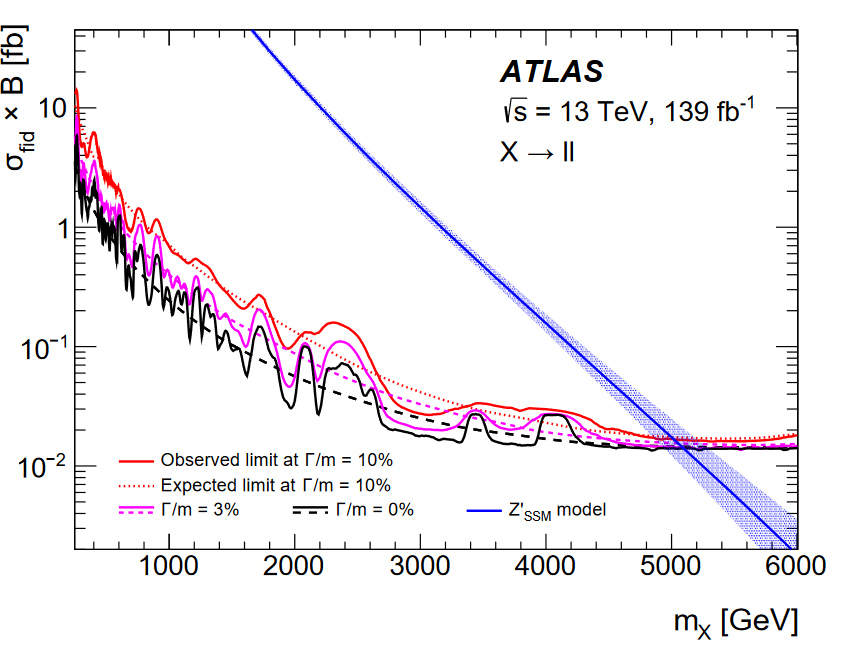
\includegraphics[width=0.6\textwidth]{Atlas_BLSM_2.png}
		\end{figure}	
		%%%%%%%%%%%%%%%%%%%%%%%%%
		
\begin{itemize}
	\item Can the minimal B-L SM still address the muon $\left(g-2\right)_\mu$ anomaly and how well? 
\end{itemize}		
		
\end{frame}


\begin{frame}{Scalar sector}
	
    \begin{equation*}
    \label{eq:potential}
    V(H,\chi)= m^2 H^\dagger H + \mu^2 \chi^\ast \chi + \lambda_1 (H^\dagger H)^2 + \lambda_2 \left(\chi^\ast \chi\right)^2 + \lambda_3  \chi^\ast \chi H^\dagger H
    \end{equation*}
	%
	\begin{itemize}
		 \item Boundedness from below: $4 \lambda_1 \lambda_2 - \lambda_3^2 >0$ and $\lambda_1,\lambda_2 > 0$
	\end{itemize}
		
	\begin{equation*}
	\begin{aligned}
	 H = \dfrac{1}{\sqrt{2}} 
		\begin{pmatrix}
		-i \left(\omega_1 - i \omega_2 \right) \\
		v + (h + i z)
		\end{pmatrix}	
		\qquad
		\chi = \dfrac{1}{\sqrt{2}} \left[ x + \left(h^\prime + i z^\prime\right) \right]	
	\end{aligned}
	\end{equation*}	

    \begin{itemize}
    	\item $\omega^\pm = \omega_1 \mp i \omega_2$, $z$ and $z^\prime$ are Goldstone bosons eaten by $W^\pm$, $Z$ and $Z^\prime$
    \end{itemize}		
    
    \begin{equation*}
    \begin{aligned}
    \mean{H} = \dfrac{1}{\sqrt{2}} 
    \begin{pmatrix}
    0 \\
    v 
    \end{pmatrix}	
    \qquad
    \mean{\chi} = \dfrac{x}{\sqrt{2}}
    \qquad \Rightarrow \qquad
    \begin{cases}
    v^2 = \tfrac{-\lambda_2 m^2 + \tfrac{\lambda_3}{2}\mu^2}{\lambda_1 \lambda_2 - \tfrac{1}{4}\lambda_3^2} > 0 \\
    x^2 = \tfrac{-\lambda_1 \mu^2 + \tfrac{\lambda_3}{2}m^2}{\lambda_1 \lambda_2 - \tfrac{1}{4}\lambda_3^2} > 0
    \end{cases}	
    \end{aligned}
    \end{equation*}			
    
    \end{frame}
    
    %%%%%%%%%%%%%%%%%%%%%%%%%%%%%

\begin{frame}
	
	\begin{columns}
		\column{.5\textwidth}
		\begin{equation*}
		\begin{aligned}
		\begin{cases}
		\lambda_2 m^2 < \tfrac{\lambda_3}{2} \mu^2 \\
		\lambda_1 \mu^2 < \tfrac{\lambda_3}{2} m^2 \\
		4 \lambda_1 \lambda_2 - \lambda_3^2 >0 \\
		\lambda_1,\lambda_2 > 0
		\end{cases}	
		\end{aligned}
		\end{equation*}
		\column{.5\textwidth}
		\begin{itemize}
			\item[] \xmark: There is no solution
			\item[] \checkmark: There is solution
		\end{itemize}
		
	\end{columns}
						
	%
	\begin{table}[htb!]
		\begin{center}
			\begin{tabular}{ccccc}
				\toprule                     
				& $\mu^2 > 0$ & $\mu^2 > 0$ & $\mu^2 < 0$ & {\red $\mu^2 < 0$}  	\\
				& $m^2 > 0$ & $m^2 < 0$ & $m^2 > 0$ & {\red $m^2 < 0$}  	\\        
				\midrule
				$\lambda_3 < 0 $     			    							& \xmark		& \checkmark	&	\checkmark & {\red \checkmark}	\\
				& 		& 	&	 & 	\\
				$\lambda_3 > 0$     			    							& \xmark		& \xmark	&	\xmark & {\red \checkmark}	\\
				\bottomrule
			\end{tabular} 
			%	\caption{\it{Charge assignment of the singlets, doublets and bi-doublets under the accidental symmetries. All three families are implicit.}}
			%	\label{tab:AccSym}  
		\end{center}
	\end{table} 
	%
%\pause
\vskip3mm
	\begin{equation*}
	\begin{aligned}
	\begin{pmatrix}
	h_1 \\
	h_2 
	\end{pmatrix}
	=
	\begin{pmatrix}
	\cos \alpha_h & -\sin \alpha_h \\
	\sin \alpha_h & \cos \alpha_h 
	\end{pmatrix}
	\begin{pmatrix}
	h \\
	h^\prime 
	\end{pmatrix}
	\end{aligned}
	\end{equation*}
	\vskip0.1mm
	{\bf Heavy $Z^\prime$ implies that $\bm{x \gg v}$ for most of the parameters points:}
	\begin{equation*}
	\sin \alpha_h \approx \dfrac{1}{2}\dfrac{\lambda_3}{\lambda_2} \dfrac{v}{x} \qquad
		m_{h_1}^2 \approx 2 \lambda_1 v^2 \qquad m_{h_2}^2 \approx 2 \lambda_2 x^2
	\end{equation*}

\end{frame}

\begin{frame}{Gauge Kinetic Mixing}
	
		\begin{equation*}
		\begin{aligned}
		\mathcal{L}_\mathrm{bosons} =  \abs{D_\mu H}^2 + \abs{D_\mu \chi}^2 - V\left(H,\chi\right) -\dfrac{1}{4} F_{\mu \nu} F^{\mu \nu} -\dfrac{1}{4} F^\prime_{\mu \nu} F^{\prime \mu \nu} -\dfrac{1}{2} \kappa F_{\mu \nu} F^{\prime \mu \nu}
		\end{aligned}
		\end{equation*}
	
			\begin{itemize}
				\item $\kappa$ is a ${\green \U{Y}} \times {\red \U{B-L}}$ gauge
				kinetic-mixing parameter
				\vskip2mm
				\item Field strength tensors ${\green F_{\mu \nu} = \partial_\mu A_\nu - \partial_\nu A_\mu}$ and ${\red F^\prime_{\mu \nu} = \partial_\mu A^\prime_\nu - \partial_\nu A^\prime_\mu}$
				\item {\blue Redefine $\kappa = \sin \alpha$ and gauge fields as (convenient basis choice)}
				\begin{equation*}
				\begin{pmatrix}
				A_\mu \\
				A^\prime_\mu 
				\end{pmatrix}
				=
				\begin{pmatrix}
				1 & -\tan \alpha \\
				0 & \sec \alpha 
				\end{pmatrix}
				\begin{pmatrix}
				B_\mu \\
				B^\prime_\mu 
				\end{pmatrix}\,,
				\label{eq:trans-kappa}
				\end{equation*}	
				\item Kinetic terms acquire canonical form
				\begin{equation*}
				\begin{aligned}
				\mathcal{L}_\mathrm{kinetic} =   -\dfrac{1}{4} B_{\mu \nu} B^{\mu \nu} -\dfrac{1}{4} B^\prime_{\mu \nu} B^{\prime \mu \nu}
				\end{aligned}
				\end{equation*}					
			\end{itemize}
			
	
\end{frame}

\begin{frame}
	
	
	\textbf{Redefined covariant derivative absorbs the kinetic mixing information:}
	
	\begin{equation*}
	\begin{aligned}
	D_\mu = \partial_\mu + i \left(g_Y \; Y + g_{BY} \; Y_{B-L}\right) B_\mu + i \left(g_{BL} \; Y_{B-L} + g_{YB} \; Y\right) B_\mu^\prime
	\end{aligned}
	\end{equation*}	
	\vskip2mm
	\begin{itemize}
		\item $g_1$ and $g_1^\prime$ are $\U{Y}$ and $\U{B-L}$ gauge couplings
		\vskip2mm
		\item $g_{YB}$ and $g_{BY}$ result from the kinetic mixing
\vskip2mm
		\item With our basis choice
		 $$\begin{cases}
				g_Y = g_1 \\
				{\blue g_{BL} = g_1^\prime \sec \alpha} \\
				{\red g_{YB} = -g_1 \tan \alpha }\\
			    g_{BY} = 0
		\end{cases} 
		\qquad
		\text{No mixing limit:}\quad \sec \alpha = 1 \Rightarrow {\blue g_{BL} = g_1^\prime}$$
	\end{itemize}

\end{frame}

\begin{frame}
	\begin{exampleblock}{}
		{\bf \begin{center} Gauge kinetic-mixing induces mixing between $Z^\prime$, $Z$ and $\gamma$ \end{center} }
	\end{exampleblock} 
	
	\begin{equation*}
	\begin{aligned}
	\begin{pmatrix}
	\gamma_\mu \\
	Z_\mu \\
	Z^\prime_\mu
	\end{pmatrix}
	=
	\begin{pmatrix}
	\cos \theta_W & \sin \theta_W & 0\\
	-\sin \theta_W \cos \theta_W^\prime & \cos \theta_W \cos \theta_W^\prime & \sin \theta_W^\prime \\
	\sin \theta_W \sin \theta_W^\prime & -\cos \theta_W^\prime \sin \theta_W^\prime & \cos \theta_W^\prime
	\end{pmatrix}
	\begin{pmatrix}
	B_\mu \\
	A^3_\mu \\
	B^\prime_\mu
	\end{pmatrix}
	\end{aligned}
	\end{equation*}	
	$$ \text{Again in the limit $x \gg v$ \qquad } \sin \theta_W^\prime \approx \dfrac{1}{8
		} \dfrac{g_{YB}}{g_{BL}}\left(\dfrac{v}{x}\right)^2 \sqrt{g^2 + g_Y^2}$$
	\begin{itemize}
		\item $g$ is $\SU{2}{L}$ gauge coupling
		\vskip2mm
		\item $\sin \theta_W^\prime = 0$ for no kinetic mixing, $g_{YB} = 0$, and {\red $Z_\mu^\prime = B_\mu^\prime$}
		\begin{itemize}
			\item For $g_{YB} = 0$ we have $m_Z = \tfrac{1}{2} v \sqrt{g^2 + g_Y^2}$ and ${\red m_{Z^\prime} \approx 2 g_{BL} x}$
			\item For $x \gg v$ we also have ${\red m_{Z^\prime} \approx 2 g_{BL} x}$
		\end{itemize}
	\end{itemize}
	
\end{frame}

\begin{frame}{Yukawa sector}
	\begin{equation*}
	\begin{aligned}
	\mathcal{L}_\mathrm{Yukawa} = & 
	-y_u^{ij} \overline{q_\mathrm{L i}} u_\mathrm{R j} \widetilde{H} 
	-y_d^{ij} \overline{q_\mathrm{L i}} d_\mathrm{R j} H
	-y_e^{ij} \overline{\ell_\mathrm{L i}} e_\mathrm{R j} H \\ &
	{\red - y_\nu^{ij} \overline{\ell_\mathrm{L i}} \nu_\mathrm{R j} \widetilde{H}
		-\dfrac{1}{2} y_M^{ij} \overline{\nu_\mathrm{R i}^c} \nu_\mathrm{R j} \chi} + \mathrm{H.c.}
	\end{aligned}
	\end{equation*}
	\begin{itemize}
		\item $\widetilde{H} = i \sigma^2 H^*$
		\vskip2mm
		\item Dirac and Majorana masses matrices: $\bm{m_D} = \tfrac{\bm{y_\nu}}{\sqrt{2}} v$ and $\bm{M} = \tfrac{\bm{y_M}}{\sqrt{2}} x$
		\item Neutrino masses via see-saw mechanism: $\begin{pmatrix}
		0 & m_D \\
		m_D & M\\
		\end{pmatrix} \rightarrow 
		\begin{cases}
		m_{\nu_l} \approx \tfrac{m_D^2}{M}\\
		m_{\nu_h} \approx M
		\end{cases}$
		\item Small mixing angle: $\tan \alpha_\nu \approx -2 \sqrt{\tfrac{m_{\nu_l}}{m_{\nu_h}}}$
	\end{itemize}
	
\end{frame}



\begin{frame}
	Four-fermion contact interactions constrain $\g{B-L}{} < 1.3$ in the B-L SM
	%%%%%%%%%%%%%%%%%%%%%%%%%
	\begin{figure}[!h]
		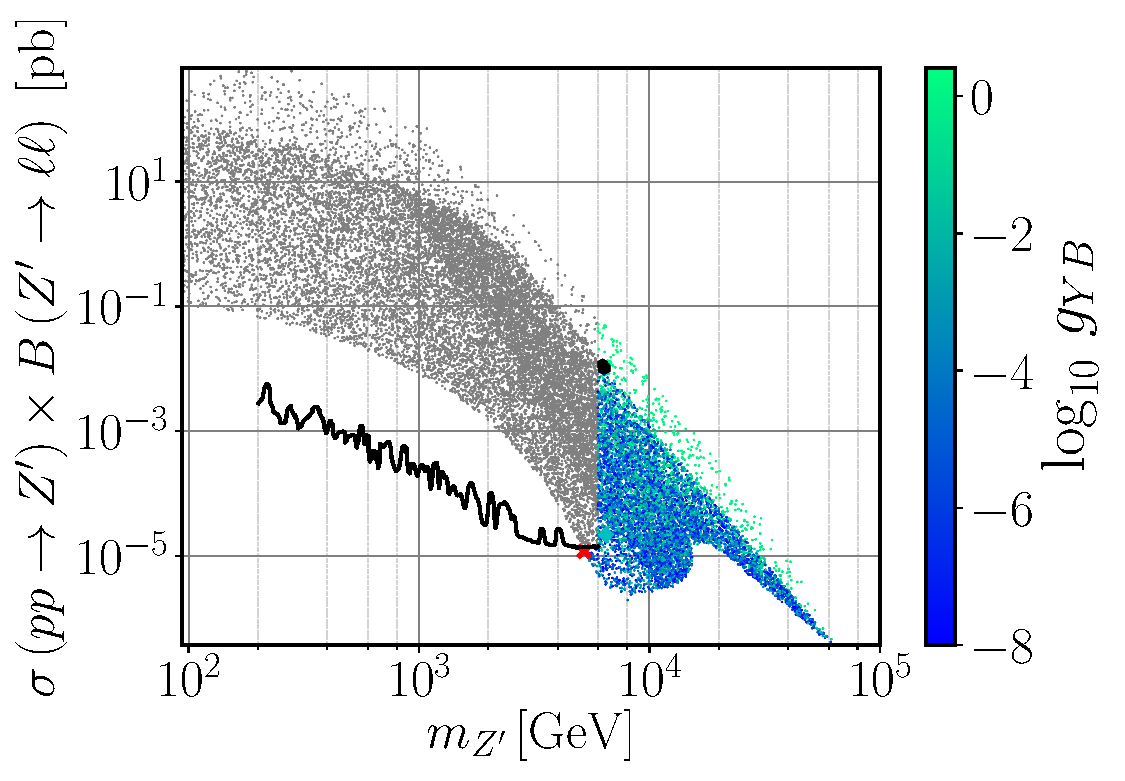
\includegraphics[width=0.40\textwidth]{Images/BLSM_2/mZp_Xsec_gYB.pdf}
		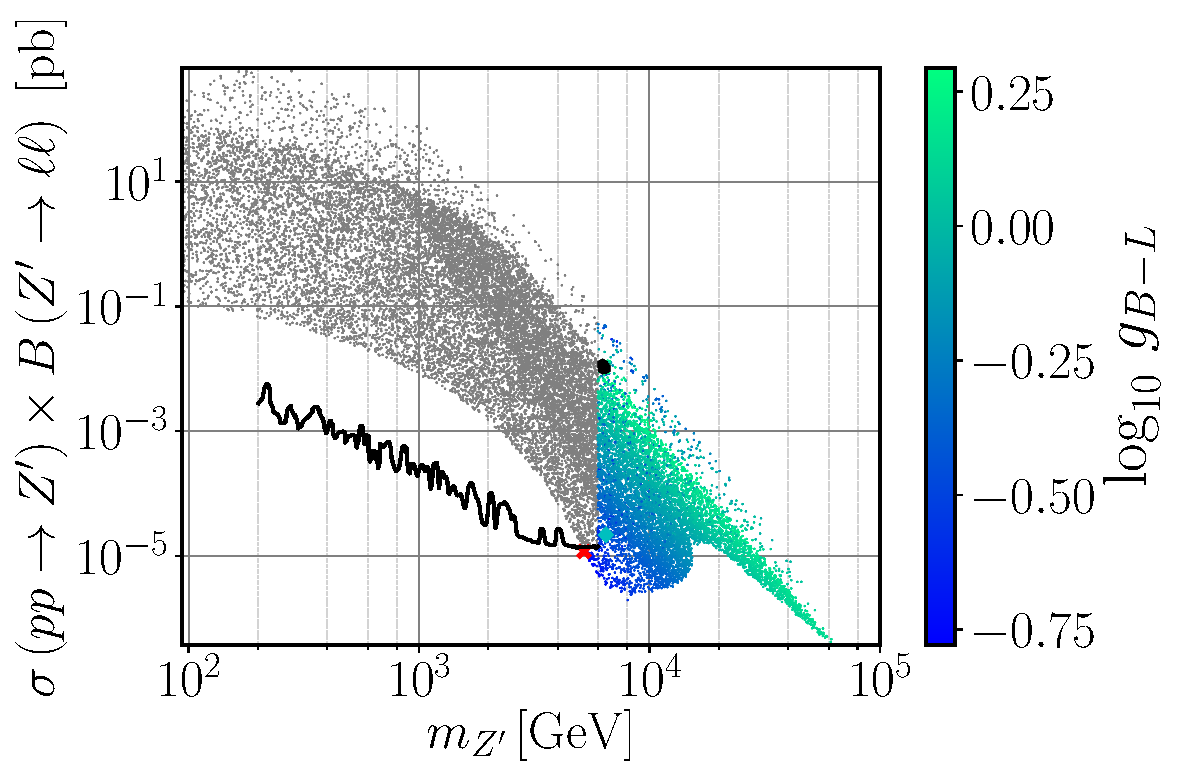
\includegraphics[width=0.40\textwidth]{Images/BLSM_2/mZp_Xsec_gBL.pdf}
	\end{figure}	
	%%%%%%%%%%%%%%%%%%%%%%%%%
	Enhancement of $\Delta a_\mu^{Z^\prime}$ is due to sizeable $\g{YB}{}$, thus large $\g{L,R}{\ell \ell Z'}$
	%%%%%%%%%%%%%%%%%%%%%%%%%
\begin{figure}[!h]
	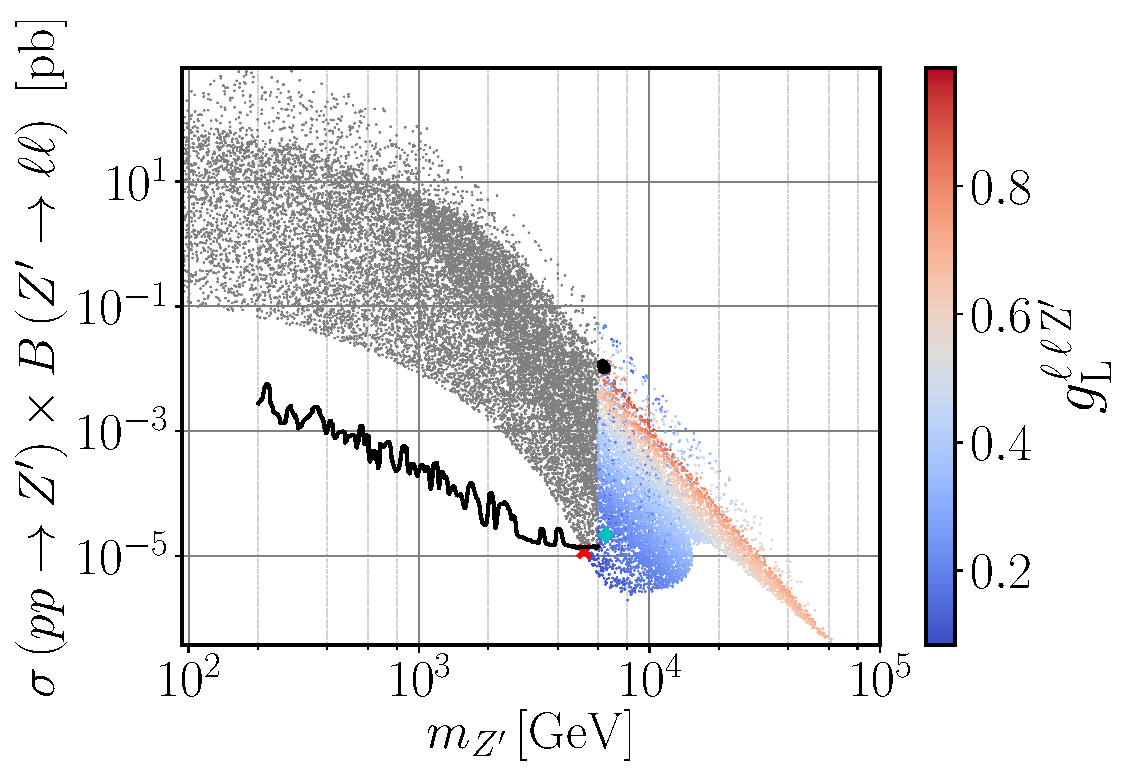
\includegraphics[width=0.40\textwidth]{Images/BLSM_2/mZp_Xsec_gLmumuZ.pdf}
	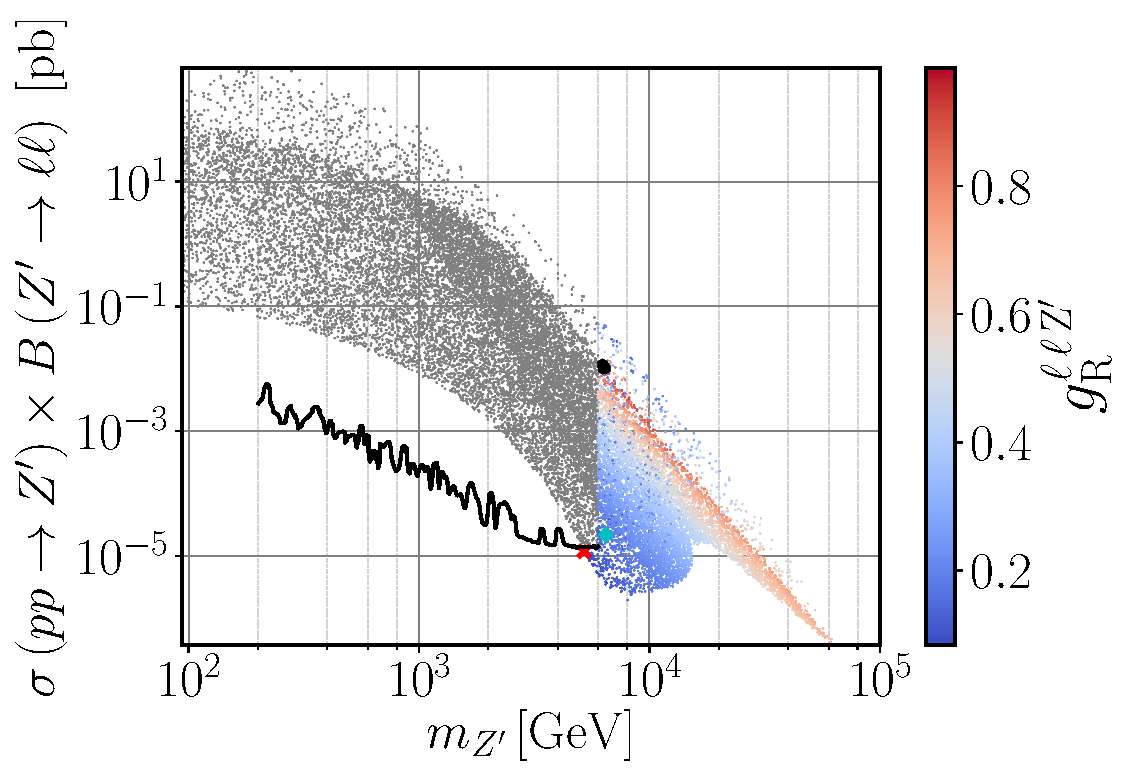
\includegraphics[width=0.40\textwidth]{Images/BLSM_2/mZp_Xsec_gRmumuZ.pdf}
\end{figure}	
%%%%%%%%%%%%%%%%%%%%%%%%%	
\end{frame}

\begin{frame}
	LEP constraints set upper bound $\sin \theta_W^\prime \lesssim 10^{-3}$
	$$\sin \theta_W^\prime \approx \dfrac{1}{8
	} \dfrac{g_{YB}}{g_{BL}}\left(\dfrac{v}{x}\right)^2 \sqrt{g^2 + g_Y^2}$$
which is respected even for the larger values of $\g{YB}{}$:	%%%%%%%%%%%%%%%%%%%%%%%%%
\begin{figure}[!h]
	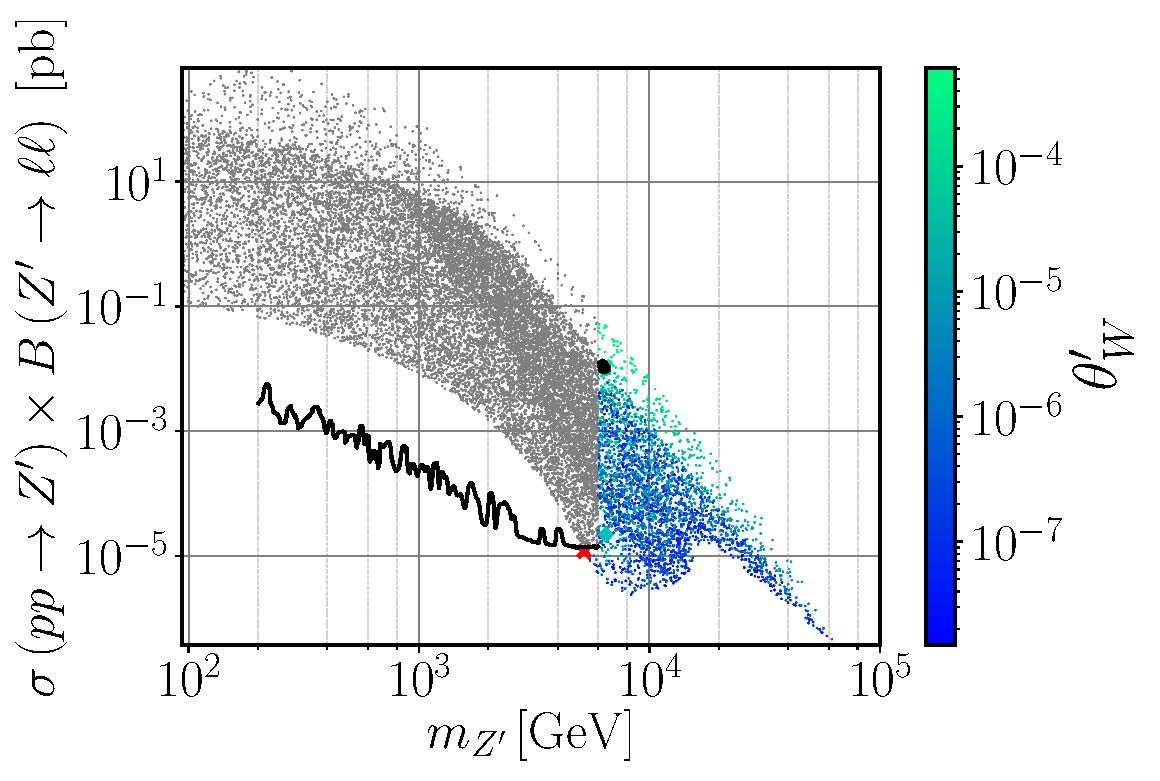
\includegraphics[width=0.45\textwidth]{Images/BLSM_2/mZp_Xsec_twp.pdf}
	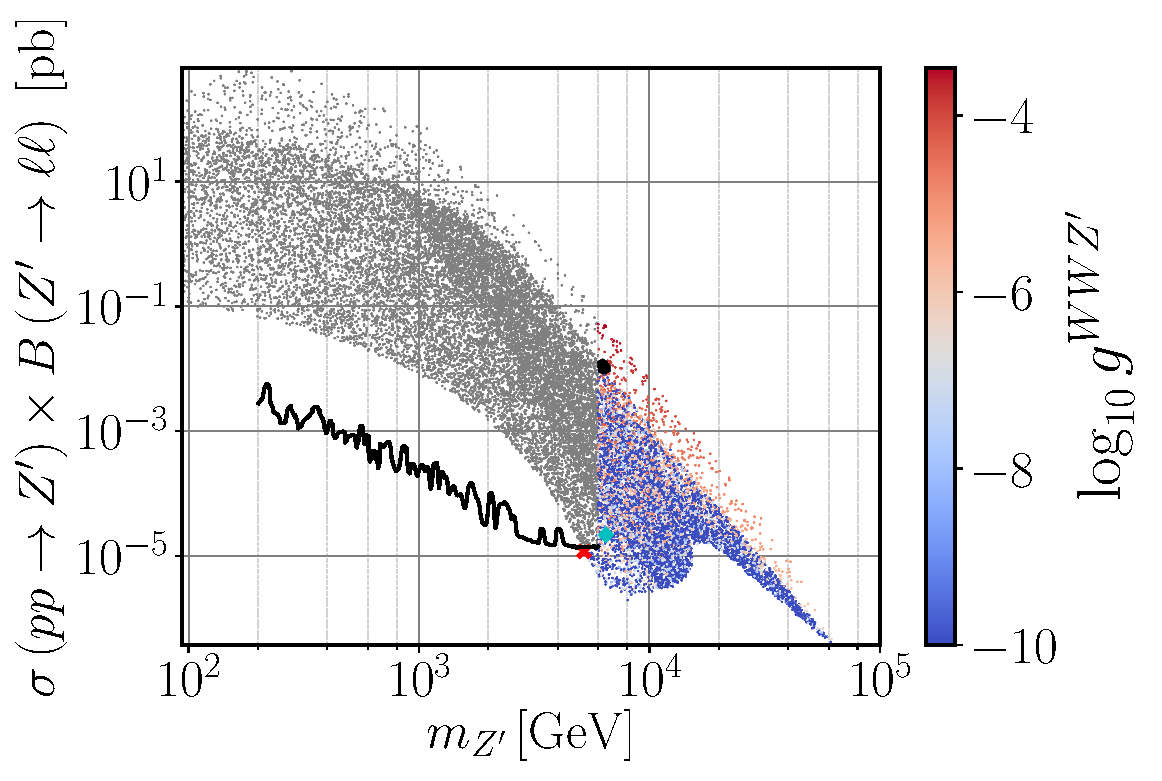
\includegraphics[width=0.45\textwidth]{Images/BLSM_2/mZp_Xsec_gWWZp.pdf}
\end{figure}	
%%%%%%%%%%%%%%%%%%%%%%%%%
Small coupling of $Z'$ to $W$ bosons: $g^{WWZ^\prime} \simeq \dfrac{1}{16} \dfrac{\g{YB}{}}{\g{B-L}{}} \left(\dfrac{v}{x}\right)^2\,.$
\end{frame}

\begin{frame}
Two-loop Barr-Zee type contributions are subdominant
%%%%%%%%%%%%%%%%%%%%%%%%%
\begin{figure}[!h]
	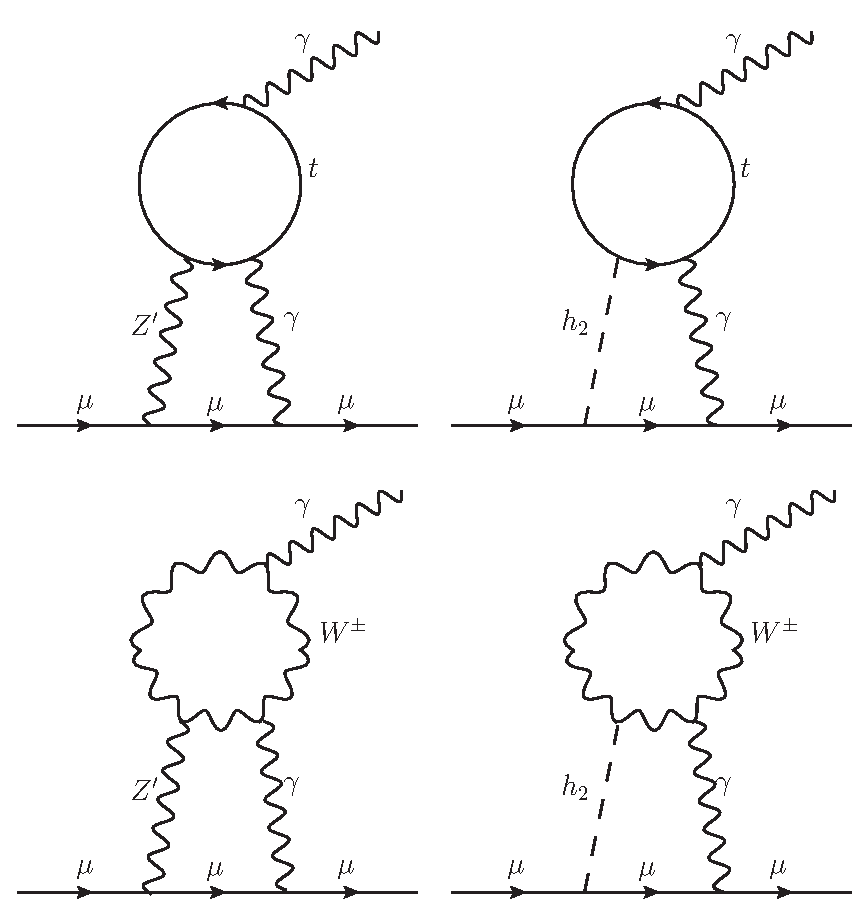
\includegraphics[scale=0.32]{Images/BLSM_2/Barr-Zee.pdf}
\end{figure}	
%%%%%%%%%%%%%%%%%%%%%%%%%
Larger contribution	from the top-left diagram due to $\g{L,R}{ttZ'} \gg \g{}{WWZ'}, \alpha_h$, however:
\begin{equation*}
\dfrac{\Delta a_\mu^{\text{Barr-Zee}}}{\Delta a_\mu^{Z^\prime}} \simeq -\dfrac{1}{65536 \pi^2}\dfrac{g^2 \left(g^2 + \g{Y}{2}\right) \g{YB}{3}}{\left[3 \g{B-L}{} \g{YB}{}  + 2\left(\g{B-L}{2} + \g{YB}{2} \right) \right] } \left(\dfrac{v}{x}\right)^4 \ll 1 
\end{equation*}

\end{frame}

\begin{frame}{3HDM - Introduction}{The Scalar Potential}

The generic scalar potential is extensively written as, 
\begin{equation*}
\label{eq:3HDM_Scalar_Pot}
\begin{split}
V(\phi_i) = & 
- \mu_1^2 \left( \phi^{\dagger}_1 \phi_1 \right) 
- \mu_2^2 \left( \phi^{\dagger}_2 \phi_2 \right)  
- \mu_3^2 \left( \phi^{\dagger}_3 \phi_3 \right) \\ 
& \left[ - \mu_{21}^2 \left( \phi^{\dagger}_2 \phi_1  \right) 
- \mu_{23}^2 \left( \phi^{\dagger}_2 \phi_3  \right)  
- \mu_{13}^2 \left( \phi^{\dagger}_1 \phi_3  \right) + \text{H.c.} \right]  \\
& + \lambda_1 \left( \phi^{\dagger}_1 \phi_1 \right) 
+ \lambda_2 \left( \phi^{\dagger}_2 \phi_2 \right)  
+ \lambda_3 \left( \phi^{\dagger}_3 \phi_3 \right) \\  
& + \lambda_4 \left( \phi^{\dagger}_1 \phi_1 \right)  \left( \phi^{\dagger}_2 \phi_2 \right) 
+ \lambda_5 \left( \phi^{\dagger}_1 \phi_1 \right)  \left( \phi^{\dagger}_3 \phi_3 \right)  
+ \lambda_6 \left( \phi^{\dagger}_2 \phi_2 \right)  \left( \phi^{\dagger}_3 \phi_3 \right)  \\ 
& + \lambda_7 \left( \phi^{\dagger}_1 \phi_2 \right)  \left( \phi^{\dagger}_1 \phi_2 \right)  
+ \lambda_8 \left( \phi^{\dagger}_1 \phi_3 \right)  \left( \phi^{\dagger}_3 \phi_1 \right)   
+ \lambda_9 \left( \phi^{\dagger}_2 \phi_3 \right)  \left( \phi^{\dagger}_3 \phi_2 \right)  \\
& + \lambda_{10} \Bigg\{ \left( \phi^{\dagger}_1 \phi_3 \right)^2 + \text{H.c.} \Bigg\} . 
\end{split} 
\end{equation*}

These fields acquire a VEV. 

\begin{equation*}
\phi_k = 
\begin{pmatrix}
w_k^\pm + i \, w_k^\mp \\ 
\frac{1}{\sqrt{2}}\left( v_k + h_k + i z_k \right)
\end{pmatrix}  \rightarrow \langle \phi_k \rangle = \begin{pmatrix}
0 \\ 
\frac{v_k}{\sqrt{2}}
\end{pmatrix} \quad , \quad k=\{ 1,2,3\} .  
\label{eq:3HDM_Higgs_Field_VEV} 
\end{equation*} 

\end{frame}


\begin{frame}{3HDM - Alignment Limit }{The Higgs Basis}
\begin{equation*}
\mathcal{O} = 
\begin{pmatrix}
\dfrac{v}{v_1} & \dfrac{v}{v_2}  & \dfrac{v}{v_3} \\[1.2em]
\dfrac{v_3}{v_{13}} & 0 & \dfrac{-v_1}{v_{13}} \\[1.2em]
\dfrac{v_2 v_1}{v v_{13}}  & \dfrac{v_{13}}{v} & \dfrac{v_2 v_3}{v v_{13}}  
\end{pmatrix} , 
\end{equation*}
%
where $v_{13}=\sqrt{v_1^2 + v_3^2}$ and $v=\sqrt{v_1^2 + v_2^2 + v_3^2 }$, the total magnitude.

\begin{equation*}
\begin{pmatrix}
\phi_1 \\
\phi_2 \\
\phi_3 \\
\end{pmatrix} = 
\mathcal{O} \begin{pmatrix}
h \\
H_1^\prime \\
H_2^\prime \\
\end{pmatrix} 
%
\quad , \quad 
%
\begin{pmatrix}
Z_1 \\
Z_2 \\
Z_3 \\
\end{pmatrix} = 
\mathcal{O} \begin{pmatrix}
z \\
A_1^\prime  \\
A_2^\prime  \\
\end{pmatrix} 
%
\quad , \quad 
%
\begin{pmatrix}
W_1^\pm  \\
W_2^\pm  \\
W_3^\pm  \\
\end{pmatrix} = 
\mathcal{O} \begin{pmatrix}
\omega^\pm \\
H_1^{\pm \prime}  \\
H_2^{\pm \prime}  \\
\end{pmatrix} . 
\end{equation*}
%
These VEVs can also be parameterized through their mixing. 
\begin{equation*}
v_1 = v \cos(\psi_1) \cos(\psi_2) \quad , \quad v_2 = v \sin(\psi_1) \cos(\psi_2) \quad , \quad v_3 = v \sin(\psi_2) , 
\end{equation*}
\end{frame}


\begin{frame}{3HDM - Alignment Limit }{Inversion Process in detail and the CP-even case}
    \textbf{Unlike in the SM, for this model we scan over the physical parameters} 
    \begin{itemize}
        \item This implies inverting all Lagrangian parameters and re-write the degrees of freedom as physical parameters.
        \item Trough this we set more than just the Higgs mass and VEV conditions but also apriori set boundess from bellow and ensure a positive mass spectrum.  
    \end{itemize}
    
    
    To reach those equations we write the mass eigenstates in the Higgs basis. Presenting the case of the scalars,
    \begin{equation*}
    \scalebox{0.8}{$
    V \supset \left( \begin{array}{ccc} 
    h_1 & h_2 & h_3 
    \end{array} \right) 
    \frac{M_S^2}{2} \left( \begin{array}{c}
    h_1 \\ 
    h_2 \\
    h_3
    \end{array} \right)$} \ ,  
    \end{equation*}
    The elements of this matrix are written as,
    %
    \begin{equation*}
    M_S^2 = 
    \scalebox{0.7}{$
    	\begin{pmatrix}
    	\frac{2 \lambda_1 v_1^3 +\mu_{21}^2 v_2 + \mu_{13}^2 v_3}{v_1} & v_1  v_2 (\lambda_4+\lambda_7)-\mu_{21}^2 & v_1
    	v_3 (2 \lambda_{10} + \lambda_5 + \lambda_8) - \mu_{13}^2 \\
    	v_1 v_2 ( \lambda_4 +\lambda_7) - \mu_{21}^2 & \frac{\mu_{21}^2 v_1+2 \lambda_2 v_2^3 +\mu_{23}^2 v_3}{v_2} & v_2
    	v_3 (\lambda_6+\lambda_9)-\mu_{23}^2 \\
    	v_1 v_3 (2 \lambda_{10}+\lambda_5+\lambda_8)-\mu_{13}^2 & v_2 v_3 (\lambda_6+\lambda_9)-\mu_{23}^2 & \frac{\mu_{13}^2 v_1+\mu_{23}^2 v_2 +2 \lambda_3 v_3^3}{v_3} \\
    	\end{pmatrix}$}.
    \end{equation*}
    %
    %With $\mathcal{O}_\alpha$ we can diagonalize the $\mathcal{CP}$-even scalar mass matrix as,. 
    %\begin{equation*}
    %\label{Eq:Generic_3HDM_eq}
    %\mathcal{O}_\alpha \underbrace{\mathcal{O} M^2_S \mathcal{O}^T }_{B_S^2} \mathcal{O}_\alpha^T \equiv \text{diag}(m_h,m_{H_1},m_{H_2}) \ . 
    %\end{equation*}
\end{frame}



\begin{frame}{3HDM - BGL-like treatment Limit }{Yukawa terms and the effect of the flavour symmetry}
    In the 3HDM the Yukawa interactions are given by,
    \begin{equation*} 
    \label{eq:3HDM_Yuk} 
    \begin{split} 
    \mathcal{L}_Y = - & \sum_{k=1}^3 \left[ \overline{Q}_{L_a} \left( \Gamma_k \right)_{ab} \phi_k n_{R_b} + \overline{Q}_{L_a} \left( \Delta_k \right)_{ab} \tilde{\phi}_k p_{R_b} + \text{H.c}.  \right] \\ + & \left( \Psi_{L_a} \left( Y^e_1 \right)_{ab} \phi_1 e_{R_b} + \text{H.c} \right) .
    \end{split} 
    \end{equation*} 
    %
    The imposed symmetry, $\mathrm{U}(1)\times\mathbb{Z}_2$, forces the Yukawa textures,  
    %
    \begin{equation*}
    \begin{aligned}
    \label{Lovely_Equations}
    &\Gamma_1  = \begin{pmatrix}
    0 & 0 & 0\\
    0 & 0 & 0\\
    \times & \times & 0
    \end{pmatrix}, \quad 
    &&\Gamma_2  = \begin{pmatrix}
    \times & \times & 0\\
    \times & \times & 0\\
    0 & 0 & 0
    \end{pmatrix}, \quad
    \Gamma_3  = \begin{pmatrix}
    0 & 0 & 0\\
    0 & 0 & 0\\
    0 & 0 & \times
    \end{pmatrix}, \\[1em]
    &\Delta_1  = \begin{pmatrix}
    0 & 0 & 0\\
    0 & 0 & 0\\
    0 & 0 & 0
    \end{pmatrix}, \quad 
    &&\Delta_2 = \begin{pmatrix}
    \times & \times & 0\\
    \times & \times & 0\\
    0 & 0 & 0
    \end{pmatrix} , \quad 
    \Delta_3 = \begin{pmatrix}
    0 & 0 & 0\\
    0 & 0 & 0\\
    0 & 0 & \times
    \end{pmatrix}  \, . 
    \end{aligned} 
    \end{equation*}
\end{frame}

\begin{frame}{3HDM - FCNCs and the suppression mechanism}
%The mass eigenstates for the negative and positive quarks can be written as,
%\begin{equation*}
%\label{eq:3HDM_Quark_gauge_mass}
%\begin{split}
%M_n = \frac{v_1}{\sqrt{2}} \Gamma_1 +  \frac{v_2}{\sqrt{2}} \Gamma_2 +  \frac{v_3}{\sqrt{2}} \Gamma_3  \quad , \\ 
%M_p = \frac{v_1}{\sqrt{2}} \Delta_1 +  \frac{v_2}{\sqrt{2}} \Delta_2 +  \frac{v_3}{\sqrt{2}} \Delta_3   \quad .
%\end{split}
%\end{equation*}

%Note, these matrices are not diagonal. So, by following the same procedure as before, we can write, 
%
The shape of the Yukawa couplings affect the mass eigenstates, we can write the following relations between the Higgs basis and physical states. 
\begin{equation*}
\scalebox{0.8}{$
m_u^{\text{diag}} = V_L^n M_n V_R^n \equiv V_L^n \begin{pmatrix}
\times & \times & 0 \\
\times & \times & 0 \\
0 & 0 & \times 
\end{pmatrix}  V_R^n  \quad , \quad 
m_d^{\text{diag}} = U_L^p  M_p U_R^p \equiv U_L^p \begin{pmatrix}
\times & \times & 0 \\
\times & \times & 0 \\
\times & \times & \times \\ \end{pmatrix} U_R^p . 
$}
\end{equation*}
Where we define the unitary matrices as to include the complex phase in there,

\begin{equation*}
\scalebox{0.8}{$
V^{n}_{L} = \begin{pmatrix}
\times & \times & 0 \\ 
\times & \times & 0 \\
0 & 0 & 1 \\ 
\end{pmatrix} \quad , \quad   V^{n}_{R} = \begin{pmatrix}
\times & \times & 0 \\ 
\times & \times & 0 \\
0 & 0 & e^{i\alpha}  \\ 
\end{pmatrix}  \quad , \quad 
U^{p}_{L,R} = 
\begin{pmatrix}
\times & \times & \times \\ 
\times & \times & \times \\
\times & \times & \times \\
\end{pmatrix} .
$}
\end{equation*}

%\begin{equation*}
%    V_{CKM} = V_L^n U_L^{p\, \dagger}
%\end{equation*}
\end{frame}

\begin{frame}{Suppression of the FCNCs in the 3HDM}
Let us then look at the rotated Yukawa interactions for the neutral Higgs. 
%
\begin{equation*}
\mathcal{L}^{H_1^\prime \, , \, H_2^\prime}_Y = 
\frac{H_1^\prime}{v} \overline{n}_L N_{d\,1} n_R + 
\frac{H_2^\prime}{v} \overline{n}_L N_{d\,2} n_R + 
\text{H.c.} \ . 
\end{equation*} 
% 
%where the matrix terms $N_{d\,1}$ and $N_{d\,2}$ can be shown to lead us to, Eq.\,(\ref{Eq:3HDM_:)}) through the use of Eq.~(\ref{3HDM_states}).   
\begin{equation*}
\label{Eq:3HDM_:)}
\begin{split}
N_{d\,1} = & \frac{v}{\sqrt{2} v_{13}} V_L^{n \, \dagger} \left( \Gamma_1 v_3 - \Gamma_3 v_1 \right) V_R^{n} \ , \\ 
N_{d\,2} = & V_L^{n \dagger} \left[ \frac{v_2}{v_{13}} \frac{1}{\sqrt{2}} \left( \gamma_1 v_1 + \gamma_3 v_3 \right) - \frac{v_{13}}{v_2} \frac{1}{\sqrt{2}} \Gamma_2 v_2  \right] V_R^n \ . 
\end{split} 
\end{equation*}
%We can now simplify Eq.~(\ref{Eq:3HDM_:)}) using the textures of the Yukawas matrices in Eq.~(\ref{Lovely_Equations}). Keeping the third row of $U_L$ the same as the \text{CKM} matrix, we can write the down sector Yukawa matrices as: 
%in the down sector sector Yukawa matrices write, 
\begin{equation*}
\Gamma_3 = (\Gamma_3)_{33} P \quad , \quad \frac{1}{\sqrt{2}}  \left( \Gamma_1 v_3 - \Gamma_3 v_1 \right) =  P M_d \ .  
\end{equation*}
Hence, 
\begin{equation*}
\begin{split}
(N_{d\,1})_{ij} = & \frac{v v_3}{v_1 v_{13}} (V_{\text{CKM}}^{\ast})_{3i} V_{\text{CKM}}^{3j} (M_d)_{jj} - \frac{1}{\sqrt{2}} \frac{v v_{13}}{v_1} ( \Gamma_3 )_{33} (V_{CKM}^{\**})_{3i} (V_R^n)_{3j},  \\ 
(N_{d\,2})_{ij} = & \frac{v_{13}}{v_2} ( M_d )_{jj} \delta_{ij} + \left( \frac{v_{13}}{v_2} + \frac{v_2}{v_{13}} \right) (V^{\**}_{\text{CKM}})_{3i} V_{\text{CKM}}^{3j} (M_d)_{jj}. 
\label{Eq:3HDM_self_;)}
\end{split} 
\end{equation*}
%
\end{frame}

\end{document}
